\PassOptionsToPackage{unicode=true}{hyperref} % options for packages loaded elsewhere
\PassOptionsToPackage{hyphens}{url}
\PassOptionsToPackage{dvipsnames,svgnames*,x11names*}{xcolor}
%
\documentclass[12pt,a4paper,openany,twoside]{report}
\usepackage{lmodern}
\usepackage{amssymb,amsmath}
\usepackage{ifxetex,ifluatex}
\usepackage{fixltx2e} % provides \textsubscript
\ifnum 0\ifxetex 1\fi\ifluatex 1\fi=0 % if pdftex
  \usepackage[T1]{fontenc}
  \usepackage[utf8]{inputenc}
  \usepackage{textcomp} % provides euro and other symbols
\else % if luatex or xelatex
  \usepackage{unicode-math}
  \defaultfontfeatures{Ligatures=TeX,Scale=MatchLowercase}
\fi
% use upquote if available, for straight quotes in verbatim environments
\IfFileExists{upquote.sty}{\usepackage{upquote}}{}
% use microtype if available
\IfFileExists{microtype.sty}{%
\usepackage[]{microtype}
\UseMicrotypeSet[protrusion]{basicmath} % disable protrusion for tt fonts
}{}
\IfFileExists{parskip.sty}{%
\usepackage{parskip}
}{% else
\setlength{\parindent}{0pt}
\setlength{\parskip}{6pt plus 2pt minus 1pt}
}
\usepackage{xcolor}
\usepackage{hyperref}
\hypersetup{
            pdfauthor={Matt Nunes},
            colorlinks=true,
            linkcolor=Maroon,
            citecolor=Blue,
            urlcolor=blue,
            breaklinks=true}
\urlstyle{same}  % don't use monospace font for urls
\usepackage{color}
\usepackage{fancyvrb}
\newcommand{\VerbBar}{|}
\newcommand{\VERB}{\Verb[commandchars=\\\{\}]}
\DefineVerbatimEnvironment{Highlighting}{Verbatim}{commandchars=\\\{\}}
% Add ',fontsize=\small' for more characters per line
\usepackage{framed}
\definecolor{shadecolor}{RGB}{248,248,248}
\newenvironment{Shaded}{\begin{snugshade}}{\end{snugshade}}
\newcommand{\AlertTok}[1]{\textcolor[rgb]{0.94,0.16,0.16}{#1}}
\newcommand{\AnnotationTok}[1]{\textcolor[rgb]{0.56,0.35,0.01}{\textbf{\textit{#1}}}}
\newcommand{\AttributeTok}[1]{\textcolor[rgb]{0.77,0.63,0.00}{#1}}
\newcommand{\BaseNTok}[1]{\textcolor[rgb]{0.00,0.00,0.81}{#1}}
\newcommand{\BuiltInTok}[1]{#1}
\newcommand{\CharTok}[1]{\textcolor[rgb]{0.31,0.60,0.02}{#1}}
\newcommand{\CommentTok}[1]{\textcolor[rgb]{0.56,0.35,0.01}{\textit{#1}}}
\newcommand{\CommentVarTok}[1]{\textcolor[rgb]{0.56,0.35,0.01}{\textbf{\textit{#1}}}}
\newcommand{\ConstantTok}[1]{\textcolor[rgb]{0.00,0.00,0.00}{#1}}
\newcommand{\ControlFlowTok}[1]{\textcolor[rgb]{0.13,0.29,0.53}{\textbf{#1}}}
\newcommand{\DataTypeTok}[1]{\textcolor[rgb]{0.13,0.29,0.53}{#1}}
\newcommand{\DecValTok}[1]{\textcolor[rgb]{0.00,0.00,0.81}{#1}}
\newcommand{\DocumentationTok}[1]{\textcolor[rgb]{0.56,0.35,0.01}{\textbf{\textit{#1}}}}
\newcommand{\ErrorTok}[1]{\textcolor[rgb]{0.64,0.00,0.00}{\textbf{#1}}}
\newcommand{\ExtensionTok}[1]{#1}
\newcommand{\FloatTok}[1]{\textcolor[rgb]{0.00,0.00,0.81}{#1}}
\newcommand{\FunctionTok}[1]{\textcolor[rgb]{0.00,0.00,0.00}{#1}}
\newcommand{\ImportTok}[1]{#1}
\newcommand{\InformationTok}[1]{\textcolor[rgb]{0.56,0.35,0.01}{\textbf{\textit{#1}}}}
\newcommand{\KeywordTok}[1]{\textcolor[rgb]{0.13,0.29,0.53}{\textbf{#1}}}
\newcommand{\NormalTok}[1]{#1}
\newcommand{\OperatorTok}[1]{\textcolor[rgb]{0.81,0.36,0.00}{\textbf{#1}}}
\newcommand{\OtherTok}[1]{\textcolor[rgb]{0.56,0.35,0.01}{#1}}
\newcommand{\PreprocessorTok}[1]{\textcolor[rgb]{0.56,0.35,0.01}{\textit{#1}}}
\newcommand{\RegionMarkerTok}[1]{#1}
\newcommand{\SpecialCharTok}[1]{\textcolor[rgb]{0.00,0.00,0.00}{#1}}
\newcommand{\SpecialStringTok}[1]{\textcolor[rgb]{0.31,0.60,0.02}{#1}}
\newcommand{\StringTok}[1]{\textcolor[rgb]{0.31,0.60,0.02}{#1}}
\newcommand{\VariableTok}[1]{\textcolor[rgb]{0.00,0.00,0.00}{#1}}
\newcommand{\VerbatimStringTok}[1]{\textcolor[rgb]{0.31,0.60,0.02}{#1}}
\newcommand{\WarningTok}[1]{\textcolor[rgb]{0.56,0.35,0.01}{\textbf{\textit{#1}}}}
\usepackage{longtable,booktabs}
% Fix footnotes in tables (requires footnote package)
\IfFileExists{footnote.sty}{\usepackage{footnote}\makesavenoteenv{longtable}}{}
\usepackage{graphicx,grffile}
\makeatletter
\def\maxwidth{\ifdim\Gin@nat@width>\linewidth\linewidth\else\Gin@nat@width\fi}
\def\maxheight{\ifdim\Gin@nat@height>\textheight\textheight\else\Gin@nat@height\fi}
\makeatother
% Scale images if necessary, so that they will not overflow the page
% margins by default, and it is still possible to overwrite the defaults
% using explicit options in \includegraphics[width, height, ...]{}
\setkeys{Gin}{width=\maxwidth,height=\maxheight,keepaspectratio}
\setlength{\emergencystretch}{3em}  % prevent overfull lines
\providecommand{\tightlist}{%
  \setlength{\itemsep}{0pt}\setlength{\parskip}{0pt}}
\setcounter{secnumdepth}{5}
% Redefines (sub)paragraphs to behave more like sections
\ifx\paragraph\undefined\else
\let\oldparagraph\paragraph
\renewcommand{\paragraph}[1]{\oldparagraph{#1}\mbox{}}
\fi
\ifx\subparagraph\undefined\else
\let\oldsubparagraph\subparagraph
\renewcommand{\subparagraph}[1]{\oldsubparagraph{#1}\mbox{}}
\fi

% set default figure placement to htbp
\makeatletter
\def\fps@figure{htbp}
\makeatother

%\documentclass[12pt,openany, a4paper, twoside]{report}
\synctex=1
\usepackage{latexsym,amsfonts,amsthm,amssymb,amsmath}
\usepackage{color,comment}
%\usepackage[usenames,dvipsnames]{xcolor}

% The following packages are necessary for lnotes.sty
\usepackage{ifthen, listings, censor, hyperref, url, graphicx}
\usepackage{enumerate}
%\input{lnotes.sty}
\usepackage[margin=1in]{geometry}

\usepackage{bm,fancyhdr}
\usepackage{natbib}
\usepackage{color}
\usepackage{outlines}
\usepackage{multirow}
\usepackage{mdframed}
%~ \usepackage[svgnames]{xcolor}
\usepackage{verbatim}
%~ \usepackage{setspace}
%~ \usepackage{sectsty}
%\allsectionsfont{\sffamily\huge}
%~ \allsectionsfont{\sffamily}
  %~ \usepackage{helvet}

\usepackage{subfig}
\usepackage{wrapfig}
\usepackage{rotating}

%\usepackage{tikz}
%\usetikzlibrary{positioning}

%%%%%%%%%%%%%%%%%%%%%%%%%%%%%%%%%%%%%%%%%%%%%%%%%%%%%%%%%%%%%%%%%%%%%%
%% Metadata
%%%%%%%%%%%%%%%%%%%%%%%%%%%%%%%%%%%%%%%%%%%%%%%%%%%%%%%%%%%%%%%%%%%%%%

\def\module{MA30234} 
\def\modulename{Statistics for Business II}

%~ \subtitle{}
%\def\logo{uob-grey}

\def\myname{Dr. Matthew Nunes} 
\def\email{m.a.nunes@bath.ac.uk} 
%\title{\modulename}

\def\uniterm{Semester 1 2020-21}

%%%%%%%%%%%%%%%%%%%%%%%%%%%%%%%%%%%%%%%%%%%%%%%%%%%%%%%%%%%%%%%%%%%%%%
%% Various template options 
%%%%%%%%%%%%%%%%%%%%%%%%%%%%%%%%%%%%%%%%%%%%%%%%%%%%%%%%%%%%%%%%%%%%%%

\provideboolean{thegaps}
\setboolean{thegaps}{false}

%\newcommand{\gap}[1]{{\textcolor{black}{ #1}}}  
\newcommand{\gap}[1]{\begin{mdframed}{\textcolor{black}{ #1}}\end{mdframed}}

\ifthenelse{
\boolean{thegaps}
}
{
\renewcommand{\gap}[1]{\begin{mdframed}{\textcolor{white}{ #1}}\end{mdframed}}
}

%\figdir{./Plots/}

% with the following flag, it is possible to use \figref{filename}
% instead of \figref{filename.pdf}. If you use pdf and other files then
% this must be set to 
%\provideboolean{only_pdf_figures}
%\setboolean{only_pdf_figures}{true}

%\margins{1in}
\parindent 5pt
\parskip 10pt
\renewcommand{\baselinestretch}{1.1}

%%%%%%%%%%%%%%%%%%%%%%%%%%%%%%%%%%%%%%%%%%%%%%%%%%%%%%%%%%%%%%%%%%%%%%
%% Emphasis (note that \emph, \emphb, \emphu are defined in the
%% template already for italics, bold and underline respectively
%%%%%%%%%%%%%%%%%%%%%%%%%%%%%%%%%%%%%%%%%%%%%%%%%%%%%%%%%%%%%%%%%%%%%%

% helper functions - these should not be used in the text,
% only in definitions of \emphX
\newcommand{\blue}{\textcolor{blue}}
\newcommand{\red}{\textcolor{red}} 

\usepackage{colortbl}

\definecolor{lyellow}{RGB}{255,255,224}
\definecolor{darkblue}{rgb}{0.03, 0.03, 0.3}
\definecolor{lightgrey}{rgb}{0.91, 0.91, 0.91}

% The template defines \emph \emphb \emphu as italics, bold and underline
\renewcommand{\emph}[1]{\textcolor{Emerald}{\textit{#1}}}
\newcommand{\emphi}[1]{\textit{#1}}
\newcommand{\emphr}[1]{\red{#1}}
\newcommand{\emphx}[1]{\blue{#1}}
\newcommand{\emphu}[1]{\noindent\underline{\textbf{#1}}}
%%%%%%%%%%%%%%%%%%%%%%%%%%%%%%%%%%%%%%%%%%%%%%%%%%%%%%%%%%%%%%%%%%%%%%
%% Out of template 
%%%%%%%%%%%%%%%%%%%%%%%%%%%%%%%%%%%%%%%%%%%%%%%%%%%%%%%%%%%%%%%%%%%%%%

\renewcommand{\familydefault}{\sfdefault}

\theoremstyle{definition}
\newtheorem{defn}{Definition}
\newtheorem*{defn*}{Definition}
\newtheorem{eg}[defn]{Example}
\newtheorem*{exer*}{Exercise}

\theoremstyle{remark}
\newtheorem{rk}{Remark}
\newtheorem*{rk*}{Remark}

\theoremstyle{plain}
\newtheorem{propn}[defn]{Proposition}
\newtheorem{thm}[defn]{Theorem}
\newtheorem*{thm*}{Theorem}
\newtheorem{cor}[defn]{Corollary}
\newtheorem*{cor*}{Corollary}
\newtheorem{claim}[defn]{Claim}
%\newtheorem{lemma}[defn]{Lemma}\newcommand{\kth}[1]{${#1}^{\textrm{th}}$}


\newtheoremstyle{example}{\topsep}{\topsep}%
     {}%         Body font
     {}%         Indent amount (empty = no indent, \parindent = para indent)
     {\bfseries}%Thm head font
     {}%         Punctuation after thm head
     {\newline}% Space after thm head (\newline = linebreak)
     {\thmname{#1}\thmnumber{ #2}\thmnote{ #3}}%         Thm head spec

%\theoremstyle{example} 
%\newtheorem{example}{Example}[section]

%\newenvironment{definition}[1][Definition]{\begin{trivlist}
%  \item[\hskip \labelsep {\bfseries #1}]}{\end{trivlist}}
\newcommand{\myvspace}{\vspace{0.5cm}}
%\newenvironment{mybox}{\vspace{0.5cm}\fbox}{}

%\newenvironment{mybox}{\begin{minipage}{2in}}{\end{minipage}}
\newcommand{\mybox}[1]{\begin{mdframed}\vspace{#1}\end{mdframed}}
\newcommand{\myshowbox}[1]{\vsp\vsp\begin{mdframed}\vsp\begin{center}<< #1 >> \end{center}\vsp\end{mdframed}\vsp\vsp}

%\newcommand{\nogap}[1]{{\textcolor{black}{ #1}}}

\newcommand{\vsp}{\vspace{.75cm}}
\newcommand{\vsps}{\vspace{.5cm}}
\renewcommand{\figurename}{Fig.}


\newcommand{\dimm}{\operatorname{dim}}
\newcommand{\Gam}{\operatorname{Gamma}}
\newcommand{\Binomial}{\operatorname{Binomial}}
\newcommand{\Bin}{\operatorname{Bin}}
\newcommand{\Bern}{\operatorname{Bern}}
\newcommand{\logit}{\operatorname{logit}}
\newcommand{\logistic}{\operatorname{logistic}}
\newcommand{\bin}{\operatorname{Bin}}
\newcommand{\corr}{\operatorname{corr}}
\newcommand{\Cov}{\operatorname{Cov}}
\newcommand{\E}{\mathbb{E}}
\newcommand{\R}{\mathbb{R}}
\newcommand{\indicator}{\mathbf{1}}
\newcommand{\MVN}{\operatorname{MVN}}
\newcommand{\N}{\operatorname{N}}
\newcommand{\Normal}{\operatorname{Normal}}
\newcommand{\Poisson}{\operatorname{Poisson}}
\newcommand{\Poi}{\operatorname{Poi}}
\newcommand{\se}{\operatorname{se}}
\newcommand{\Uniform}{\operatorname{Uniform}}
\newcommand{\Unif}{\operatorname{Unif}}
\newcommand{\Var}{\operatorname{Var}}
\newcommand{\cD}{\mathcal{D}}
\newcommand{\cR}{\mathcal{R}}
\newcommand{\cM}{\mathcal{M}}
\newcommand{\cMM}[2]{\mathcal{M}_{#1 \times #2}(\mathbb{R})}
\newcommand{\simiid}{\stackrel{\operatorname{iid}}{\sim}}
\newcommand{\xx}{{x_1,\dots,x_n}}
\newcommand{\XX}{{X_1,\dots,X_n}}
\newcommand{\yy}{{y_1,\dots,y_n}}
\newcommand{\YY}{{Y_1,\dots,Y_n}}
\newcommand{\ii}{{i=1,\dots,n}}
\newcommand{\Yij}{Y_{ij}}
\newcommand{\yij}{y_{ij}}
\newcommand{\epij}{\epsilon_{ij}}
\newcommand{\bmb}{\bm{\beta}}
\newcommand{\bmt}{\bm{\theta}}
\newcommand{\bmm}{\bm{\mu}}
\newcommand{\bme}{\bm{\eta}}
%\newcommand{\bmg}{\bm{\gamma}}
\newcommand{\bmg}{\bm{b}}
\newcommand{\bmB}{\bm{b}}
\newcommand{\bmX}{\bm{X}}
\newcommand{\xit}{\bm{x_i}^{T}}
\newcommand{\zit}{\bm{z_i}^{T}}
\newcommand{\ssin}{\sum_{i=1}^{n}}
\newcommand{\ssiI}{\sum_{i=1}^{I}}
\newcommand{\ssjJ}{\sum_{j=1}^{J}}
\newcommand{\Oi}{\operatorname{Observed}_i}
\newcommand{\Ei}{\operatorname{Expected}_i}
\newcommand{\sign}{\operatorname{sign}}
\newcommand{\ep}{\epsilon}
\newcommand{\nb}{&nbsp;}
%************************************************************

%\figposition{!h}

%%% STOP! 
%\let\oldmaketitle\maketitle
%\AtBeginDocument{\let\maketitle\relax}

%\newcommand{\myd}[1]{\textbf{\textit{#1}}}
\newcommand{\myd}[1]{\emphx{#1}}
\newcommand{\sR}[1]{\textbf{R}\,}

\newcommand{\bea}{
\begin{eqnarray}
        }
        \newcommand{\eea}{
\end{eqnarray}
}
\newcommand{\bean}{
\begin{eqnarray*}
        }
        \newcommand{\eean}{
\end{eqnarray*}
}

\author{Matt Nunes}
\date{2020-10-05}

\usepackage{amsthm}
\newtheorem{theorem}{Theorem}[chapter]
\newtheorem{lemma}{Lemma}[chapter]
\newtheorem{corollary}{Corollary}[chapter]
\newtheorem{proposition}{Proposition}[chapter]
\newtheorem{conjecture}{Conjecture}[chapter]
\theoremstyle{definition}
\newtheorem{definition}{Definition}[chapter]
\theoremstyle{definition}
\newtheorem{example}{Example}[chapter]
\theoremstyle{definition}
\newtheorem{exercise}{Exercise}[chapter]
\theoremstyle{remark}
\newtheorem*{remark}{Remark}
\newtheorem*{solution}{Solution}
\let\BeginKnitrBlock\begin \let\EndKnitrBlock\end
\begin{document}

\renewcommand{\maketitle}{
\thispagestyle{empty}
\vspace*{\fill}
\vspace{-7.5em}
\begin{center}
        \textcolor{black}{{\LARGE \module}}
\end{center}
\vspace{0.5em}
\begin{center}
\begin{minipage}{0.8\textwidth}
\begin{center}
        \textcolor{black}{{\Huge \modulename}}
\end{center}
\end{minipage}
\end{center}
\vspace*{7em}
\begin{center}
   \textcolor{black}{{\Large \myname}}\\
   \textcolor{black}{\texttt{\Large \email}}
\end{center}
\vspace{7em}
\begin{center}
\begin{minipage}{0.6\textwidth}
\begin{center}
        \includegraphics[width=3cm,keepaspectratio=true]{uob-grey.pdf}
\end{center}
\end{minipage}
\end{center}
\vspace*{\fill}
Adapted from original notes by Ilaria Prosdocimi / Sandipan Roy prior to 2020.
\hrule
\vspace{-0.5em}
\begin{center}
        \textcolor{black}{{\large \uniterm}\hfill {\large University of Bath}}
\end{center}
}

%\let\maketitle\oldmaketitle 
%\title{}
\maketitle

\hypertarget{general-information}{%
\chapter*{General Information}\label{general-information}}
\addcontentsline{toc}{chapter}{General Information}

Due to COVID-19, this course will be entirely online this year. However, to keep some structure for the course amongst other modules, I will be releasing video content by Wednesdays 1315 each
week -- watch out for the announcements on Moodle. Practical classes will be scheduled for Thursdays at 1315\footnote{at the time of writing}. I will hold office hours Mondays 1015--1215 -- please email for an appointment.

\hypertarget{course-outline}{%
\section*{Course Outline}\label{course-outline}}
\addcontentsline{toc}{section}{Course Outline}

This course concerns two types of real-world data modelling: regression and time series analysis (with an emphasis on forecasting). Both modelling situations arise
frequently in business applications, and the course will focus on applications in this area. The focus will be on practical aspects of these two areas, in particular statistical and computer analysis skills.

\hypertarget{aims-and-learning-outcomes}{%
\subsection*{Aims and learning outcomes}\label{aims-and-learning-outcomes}}
\addcontentsline{toc}{subsection}{Aims and learning outcomes}

To teach the methods of analysis appropriate to simple and multiple regression models; to introduce techniques for modelling and forecasting time series.

Students should be able to set up and analyse regression models and assess the resulting model critically. They should be able to model temporal data, and to provide forecasts with associated uncertainty estimates. They should be able to use \sR~and a calculator to perform analyses.

\hypertarget{content}{%
\subsection*{Content}\label{content}}
\addcontentsline{toc}{subsection}{Content}

The module will cover the following topics:

\begin{itemize}
\item
  Simple and multiple regression: estimation of model parameters, tests, confidence and prediction intervals, residual and diagnostic plots.
\item
  Practical time series analysis: time plots, trend-and-seasonal models.
\item
  Practical forecasting: Exponential smoothing, Holt's linear trend model and Holt-Winters seasonal forecasting.
\item
  Autoregressive models, Box-Jenkins ARIMA forecasting.
\end{itemize}

\hypertarget{lecture-plan}{%
\subsection*{Lecture plan}\label{lecture-plan}}
\addcontentsline{toc}{subsection}{Lecture plan}

\begin{description}
\item[Week 1:]  Revision of statistical concepts and introduction to R
\item[Weeks 2--4:] Simple linear regression 
\item[Weeks 5--6:] Multiple linear regression 
\item[Weeks 7--8:] Time series:  moving average models, exponential smoothing 
\item[Weeks 9--10:] ARIMA models
\item[Week 11:]  Some revision of key aspects of the module and advice for the coursework  
\end{description}

\hypertarget{assessment}{%
\subsection*{Assessment}\label{assessment}}
\addcontentsline{toc}{subsection}{Assessment}

\textbf{Coursework accounts for 100\% of the assessment for this module}. Both the content and the presentation style will carry a weight in the
assessment. The students will need to show that they have understood how to decide which modelling procedure is suitable for a particular situation, how to perform a
statistical analysis and will also need to show they can effectively communicate the meaning of their findings.

\hypertarget{suggested-reading-material}{%
\section*{Suggested reading material}\label{suggested-reading-material}}
\addcontentsline{toc}{section}{Suggested reading material}

\begin{itemize}
\item
  Lind, Marchal, Wathen (2008). \emph{Statistical Techniques in Business \& Economics with Global Datasets, 13th Ed.}, McGraw-Hill. \blue{L4 519.5$<$LIN$>$}.
\item
  Faraway, J. J. (2015) \emph{Linear models with R, 2nd Ed.}, Chapman \& Hall/CRC
  Press. \blue{L4 519.5$<$FAR$>$}.
\end{itemize}

\hypertarget{revision}{%
\chapter{Revision of Summations and Sampling Distributions and Introduction to R}\label{revision}}

\hypertarget{revnotation}{%
\section{Summation}\label{revnotation}}

Summation, as the name suggests, is simply the addition of a sequence of numbers. In mathematical notation, we use the Greek summation symbol \(\Sigma\) (\textit{Sigma}) for this; the index, usually \(i\) or \(j\), indicates the start and end points in the sequence where the summation should be calculated. For example, for a sequence
\(\{x_i\}_{i=1}^{n}= \{x_1, \dots, x_n\}\), if we wanted to calculate \(x_3+x_4+x_5\) it would be \(\sum_{i=3}^5 x_i\).

For sequences \(\{x_i\}_{i=1}^{n}= \{x_1, \dots, x_n\}\) and \(\{y_j\}_{j=1}^{n}=\{y_1,\dots,y_n\}\), some frequently used summations are given below:
\begin{eqnarray*}
\sum_{i=1}^n x_i &=&  x_1 + x_2 + \ldots + x_n\\
\sum_{i=1}^n y_i^2 &=&  y_1^2 + y_2^2 + \ldots + y_n^2\\
\sum_{i=1}^n x_i y_i &=&  x_1 y_1 + x_2 y_2 + \ldots + x_n y_n\\
\sum_{i=1}^n (x_i - \bar{x}) &=& (x_1 - \bar{x}) + (x_2 - \bar{x}) + \ldots + (x_n - \bar{x})\\
\sum_{i=1}^n (x_i - \bar{x})^2 &=& (x_1 - \bar{x})^2 + (x_2 - \bar{x})^2 + \ldots + (x_n - \bar{x})^2
\end{eqnarray*}

These types of summations will be used in the first part of the course.

\hypertarget{some-propertiestricks}{%
\subsection*{Some properties/tricks}\label{some-propertiestricks}}
\addcontentsline{toc}{subsection}{Some properties/tricks}

\begin{eqnarray*}
\sum_{i=1}^{n} a x_i &=& a \sum_{i=1}^{n} x_i \\
\sum_{i=1}^{n} (x_i + a) &=& \left(\sum_{i=1}^{n} x_i\right) + n a \\
\sum_{i=1}^{n} (x_i + y_i) &=& \sum_{i=1}^{n} x_i + \sum_{i=1}^{n} y_i \\
\sum_{i=1}^{n} (x_i - y_i) &=& \sum_{i=1}^{n} x_i - \sum_{i=1}^{n} y_i \\
\sum_{i=1}^{n} i &=& 1 + 2 + 3 + \ldots + (n-2) + (n-1) + n = \frac{n(n+1)}{2}
\end{eqnarray*}
\vsps

\begin{exer*}
Complete the table below:\newline

\begin{longtable}[c]{@{}lrrrlllll@{}}
\toprule
i & $x_i$ & $y_i$ &
$z_i$ &
$x_iy_i$ &
$x_iz_i$ &
$y_i-z_i$ &
$x_i - \bar{x}$ &
$(x_i - \bar{x})^2$ \tabularnewline
\midrule
\endhead
1 & \emph{1} & \emph{-1} & \emph{2} & & & & &\tabularnewline
2 & \emph{2} & \emph{-2} & \emph{4} & & & & &\tabularnewline
3 & \emph{3} & \emph{-3} & \emph{-2} & & & & &\tabularnewline
\bottomrule
$\Sigma$ & & & & & & & &\tabularnewline
\end{longtable}
\end{exer*}
\vsps

\begin{exer*}
For the sample $(x_1, \ldots ,x_{10}) = (2,5,6,7,1,9,5,1,4,5)$, compute the following summations.
\[\sum_{i=3}^{6} x_i, \quad \sum_{i=7}^{10} x_i^3 \quad \mbox{and} \quad \sum_{i=1}^{10} 3 x\].
\end{exer*}

\hypertarget{sampdist}{%
\section{Estimates and sampling distributions}\label{sampdist}}

An \myd{estimate} is our best guess at a parameter's value, based on
the data available to us. For example, suppose we assume that
\[\left\{ X_{1},X_{2},\ldots,X_{n} \right\}\]
are independently distributed \(N(\mu,\sigma^{2})\) random variables.
\(\mu\) is a \myd{parameter} representing a typical value, the mean of the
\textbf{population} of \(X\)'s we might encounter. \(\sigma^{2}\) is
another parameter, representing the variance of the same population.

\newpage

We can estimate \(\mu\) and \(\sigma^{2}\) in a variety of ways, but, based on a
sample of size \textit{n}, the most common estimates used are:
\[\hat{\mu} = \bar{x} = \frac{1}{n}\ \sum_{i = 1}^{n}x_{i}\]

and
\[{\hat{\sigma}}^{2} = \ s^{2} = \ \frac{1}{n - 1}\sum_{i = 1}^{n}{(x_{i} -\bar{x}})^{2}\]

The hat symbol \(\hat{\phantom{mu}}\) indicates we are calculating an estimate.
\vsps

\BeginKnitrBlock{example}[Estimate example]
\protect\hypertarget{exm:sumtesting}{}{\label{exm:sumtesting} \iffalse (Estimate example) \fi{} }Suppose we have a \textbf{sample} of 10 observations (\(n = 10\)) from an assumed \(N(\mu,\sigma^{2})\) population, namely:\newline

\begin{center}
\begin{tabular}{c|cccccccccc}
$i$ & 1 & 2 & 3 & 4 & 5 & 6 & 7 & 8 & 9 & 10\\ 
\hline
$x_i$ & 2.57 & 3.89 & 2.04 & 2.57 & 0.89 & 2.65 & 3.49 & -0.32 & 1.01 & 0.88
\end{tabular}
\end{center}
\vsps

You should be able to calculate
\[\hat{\mu} = \bar{x}= \frac{1}{10}\ \sum_{i = 1}^{10}x_{i} = 1.967\]
\[{\hat{\sigma}}^{2} = \ s^{2} = \ \frac{1}{9}\sum_{i = 1}^{10}{(x_{i} -\bar{x}})^{2} = 1.7449\]

So, from this particular sample of 10, we estimate \(\hat{\mu} = 1.967\)
and \(\hat{\sigma}^{2} = 1.7449\).
\EndKnitrBlock{example}
\vsps

If we selected another sample of 10 from the population, we would obtain
another, almost certainly different, estimate \(\hat{\mu}\) and another
estimate \({\hat{\sigma}}^{2}\). The variation in the value of our
estimate from sample to sample is called the \myd{sampling
distribution} of the estimate. If we know the sampling distribution of
the estimate, we can use it to build confidence intervals and carry out
hypothesis tests on the population parameters.

If \(\left\{ X_{1},X_{2},\ldots,X_{n} \right\}\) are
\(N(\mu,\sigma^{2})\) random variables with \(\sigma\) known, then
\[\bar{X}= \hat{\mu}\sim N\left(\mu,\ \frac{\sigma^{2}}{n}\right)\]

Note that:

\begin{itemize}
\item
  the distribution of \(\hat{\mu}\) has the same mean as the
  distribution of \(X_{1}\) or \(X_{2}\), but a smaller variance.
\item
  the variance of \(\hat{\mu}\) reduces as the sample size \(n\) increases
\item
  Hence, \(\bar{X}\) is a better estimate of \(\mu\)
  than a single observation, e.g. \(X_{1}\) or \(X_{2}\)
\end{itemize}

A 95\% confidence interval for \(\mu\) \textbf{based on an observed sample} \(x=(x_1,\dots,x_n)\) is therefore:
\[\bar{x} \pm 1.96\times\frac{\sigma}{\sqrt{n}}\]

If \(\sigma\) is not known, but is estimated using the sample standard
deviation, we use the \(t\)-distribution (with \((n - 1) = 9\) degrees
of freedom) to build a confidence interval for \(\mu\).
\vsps

\BeginKnitrBlock{example}[Confidence interval example]
\protect\hypertarget{exm:sumtestCI}{}{\label{exm:sumtestCI} \iffalse (Confidence interval example) \fi{} }For Example \ref{exm:sumtesting}, for instance, the 95\% confidence interval for \(\mu\) is
\[ 1.967 - t_{0.025,9}\times\sqrt{1.7449/10} < \ \mu < 1.967 + t_{0.025,9}\times\sqrt{1.7449/10} \]
i.e.
\[1.0221 < \mu < 2.9119\]
\EndKnitrBlock{example}
\vsps

We will use the sampling distributions of estimates of parameters in our analysis later in the unit.

\hypertarget{hyptest}{%
\subsection{Hypothesis testing}\label{hyptest}}

We can use the sampling distribution of an estimate of the parameter of a population to test hypotheses about the parameter.
For instance, we can hypothesise that the population mean is

\begin{itemize}
\item
  different from a value \(\mu_0\)
\item
  greater than a value \(\mu_0\)
\item
  smaller from a value \(\mu_0\)
\end{itemize}

In these cases, the hypotheses we are testing are (respectively):

\begin{itemize}
\item
  \(H_0: \mu = \mu_0\) vs. \(H_1: \mu \neq \mu_0\)
\item
  \(H_0: \mu = \mu_0\) vs. \(H_1: \mu > \mu_0\)
\item
  \(H_0: \mu = \mu_0\) vs. \(H_1: \mu < \mu_0\)
\end{itemize}

In the first case we carry out a two-tailed test; in the latter two cases we carry out a one-tailed test (right-tailed and left-tailed).

Typically a test is carried out a pre-specified type-I error rate \(\alpha\) (typical values of \(\alpha\) are 0.1, 0.05, 0.01).
The pre-specified type-I error rate indicates the level of false positives we are willing to allow in the testing procedures (i.e.~tests which reject \(H_0\) when \(H_0\) is actually true).

Alternatively one can compute the p-value corresponding to the observed test-statistic, which gives an indication of the evidence in favour of \(H_0\).
The p-value can then be compared with the pre-specified type-I error rate.

If we can assume that the sample mean is Normally distributed, either because the original data is Normally distributed, or our sample size is large enough (say,
\(n=30\) or above) AND we know the population standard deviation, then we use the Normal distribution to test the hypotheses.

If we can assume the sample mean is Normally distributed, but we have had to estimate the standard deviation using the sample standard deviation (and we have therefore
introduced additional uncertainty into our hypothesis), then we use the t-distribution to test the hypotheses.

Assuming we do not know the population variance, then we would proceed as follows in each of the cases above:

\begin{enumerate}
\def\labelenumi{\arabic{enumi}.}
\tightlist
\item
  \emph{two-sided test} \(H_0: \mu = \mu_0\) vs. \(H_1: \mu \neq \mu_0\).
\end{enumerate}

Since this is a two-sided test, if the test statistic
\[ t_{obs} = \frac{(\bar{x} - \mu_0)}{s/\sqrt{n}} > t_{1-\alpha/2, n-1} \quad {or} \quad t_{obs} = \frac{(\bar{x} - \mu_0)}{s/\sqrt{n}} < t_{\alpha/2, n-1}\]
then we reject \(H_0\). The p-value of the test can be calculated as: \(p = 2 P(T_{n-1} > |t_{obs}|)\)

\begin{enumerate}
\def\labelenumi{\arabic{enumi}.}
\setcounter{enumi}{1}
\tightlist
\item
  \emph{one-sided test} \(H_0: \mu = \mu_0\) vs. \(H_1: \mu > \mu_0\).
\end{enumerate}

Since this is a one-sided test, if the test statistic
\[ t_{obs} = \frac{(\bar{x} - \mu_0)}{s/\sqrt{n}} > t_{1-\alpha, n-1} \]
then we reject \(H_0\).
The p-value of the test can be calculated as: \(p = P(T_{n-1} > t_{obs})\)

\begin{enumerate}
\def\labelenumi{\arabic{enumi}.}
\setcounter{enumi}{2}
\tightlist
\item
  \emph{one-sided test} \(H_0: \mu = \mu_0\) vs. \(H_1: \mu < \mu_0\).
\end{enumerate}

Since this is a one-sided test, if the test statistic
\[ t_{obs} = \frac{(\bar{x} - \mu_0)}{s/\sqrt{n}} < t_{\alpha, n-1} \]
then we reject \(H_0\).
The p-value of the test can be calculated as: \(p = P(T_{n-1} < t_{obs})\)

\hypertarget{usingr}{%
\section{Using R}\label{usingr}}

We will use \sR~for different sections of this course:

\begin{itemize}
\item
  for plotting and visualising data
\item
  carrying out repetitive calculations
\item
  calculating parameter estimation
\item
  using in-built functions and packages to carry out some of the analysis itself.
\end{itemize}

It is recommended you look over the suggested \emph{Introduction to R} material on Moodle at the start of the course to reduce the time needed later for producing results for assessed coursework.

\hypertarget{r-packages}{%
\subsection{R packages}\label{r-packages}}

We will predominantly use in-built functions, as well as two \sR~add-on packages for the time series section of this course: the \texttt{astsa} package and the \texttt{tseries} package. Some additional packages may be required for specific datasets and methods, such as the \texttt{forecast} package.

Although not needed early in the course, it is suggested you make sure these are installed on your version of \sR~so they are ready for when you need them. \sR~add-on packages can be installed by:\newline

\begin{Shaded}
\begin{Highlighting}[]
\KeywordTok{install.packages}\NormalTok{( }\KeywordTok{c}\NormalTok{(}\StringTok{"astsa"}\NormalTok{, }\StringTok{"tseries"}\NormalTok{) )}
\end{Highlighting}
\end{Shaded}

\vsps

When you need to use them, load them into your \sR~workspace using for
example: \newline

\begin{Shaded}
\begin{Highlighting}[]
\KeywordTok{library}\NormalTok{(}\StringTok{"astsa"}\NormalTok{)}
\end{Highlighting}
\end{Shaded}

\hypertarget{plotting-data}{%
\subsection{Plotting data}\label{plotting-data}}

Line and scatter plots in particular are useful accompaniments to
analysis in this unit, although other types of charts (e.g.~histograms)
may also be appropriate.

To create a plot in \sR, the \texttt{plot} command is very general command which allows a graph to be drawn with different attributes. We now introduce some useful graphs types in \sR,.

\hypertarget{histograms}{%
\subsubsection*{Histograms}\label{histograms}}
\addcontentsline{toc}{subsubsection}{Histograms}

A histogram is one of the most commonly used graphs and is used to illustrate comparisons among categories or the general behaviour (distribution)
of data.\newline

\begin{Shaded}
\begin{Highlighting}[]
\CommentTok{# load in-built dataset}
\KeywordTok{data}\NormalTok{(mtcars)}

\CommentTok{# plot histogram, with a user-defined x axis label}
\KeywordTok{hist}\NormalTok{(mtcars}\OperatorTok{$}\NormalTok{hp, }\DataTypeTok{xlab =} \StringTok{"Horse power of cars in 1974"}\NormalTok{)}
\end{Highlighting}
\end{Shaded}

\begin{figure}[h]

{\centering 
\includegraphics[width=0.7\linewidth]{MA30234_files/figure-latex/mtcarhp-1} 

}

\caption{An example of a histogram using an in-built dataset using the \texttt{hist} function.}\label{fig:mtcarhp}
\end{figure}
\vsps

\hypertarget{line-graphs}{%
\subsubsection*{Line graphs}\label{line-graphs}}
\addcontentsline{toc}{subsubsection}{Line graphs}

Line Graphs are mainly used to plot changes in data over time e.g.~temperature.\newline

\begin{Shaded}
\begin{Highlighting}[]
\CommentTok{# load saved data}
\KeywordTok{load}\NormalTok{(}\StringTok{"arctic.Rdata"}\NormalTok{)}
\KeywordTok{names}\NormalTok{(minSeaIce)}
\end{Highlighting}
\end{Shaded}

\begin{verbatim}
## [1] "Year"      "IceExtent"
\end{verbatim}

\begin{Shaded}
\begin{Highlighting}[]
\CommentTok{# plot data with "b" -- both points and line }
\KeywordTok{plot}\NormalTok{(minSeaIce}\OperatorTok{$}\NormalTok{Year, minSeaIce}\OperatorTok{$}\NormalTok{IceExtent, }\DataTypeTok{xlab =} \StringTok{"Year"}\NormalTok{, }
                    \DataTypeTok{ylab =} \StringTok{"Sea Ice Extent"}\NormalTok{, }\DataTypeTok{type =} \StringTok{"b"}\NormalTok{)    }

\KeywordTok{library}\NormalTok{(astsa)}

\CommentTok{# plot in-built time series data object}
\KeywordTok{data}\NormalTok{(gtemp)}
\KeywordTok{plot}\NormalTok{(gtemp, }\DataTypeTok{ylab =} \StringTok{"Global Temperature"}\NormalTok{)}
\end{Highlighting}
\end{Shaded}

\begin{figure}[h]

{\centering 
\includegraphics[width=0.7\linewidth]{MA30234_files/figure-latex/lineplots-1} 
\includegraphics[width=0.7\linewidth]{MA30234_files/figure-latex/lineplots-2} 

}

\caption{Examples of line graphs with both general data and \texttt{ts} (time series) objects. Left: arctic sea ice; right: global annual temperature.}\label{fig:lineplots}
\end{figure}
\vsps

\hypertarget{scatter-graphs}{%
\subsubsection*{Scatter graphs}\label{scatter-graphs}}
\addcontentsline{toc}{subsubsection}{Scatter graphs}

A scatter graph is useful for plotting the relationship between two different variables.\newline

\begin{Shaded}
\begin{Highlighting}[]
\CommentTok{# load in-built dataset}
\KeywordTok{data}\NormalTok{(mtcars)}

\CommentTok{# plot scatter plot, using a different point type }
\KeywordTok{plot}\NormalTok{(mtcars}\OperatorTok{$}\NormalTok{wt, mtcars}\OperatorTok{$}\NormalTok{mpg, }\DataTypeTok{main =} \StringTok{"Scatterplot example"}\NormalTok{, }
                    \DataTypeTok{xlab =} \StringTok{"Car Weight"}\NormalTok{, }\DataTypeTok{ylab =} \StringTok{"Miles Per Gallon"}\NormalTok{, }\DataTypeTok{pch =} \DecValTok{19}\NormalTok{)}
\end{Highlighting}
\end{Shaded}

\begin{figure}[h]

{\centering 
\includegraphics[width=0.7\linewidth]{MA30234_files/figure-latex/mtcarscatter-1} 

}

\caption{An example of a scatter plot.}\label{fig:mtcarscatter}
\end{figure}
\vsps

Examples will be given in the first problem class.

\hypertarget{formulae}{%
\subsection{Formulae, Data Manipulation and Functions}\label{formulae}}

Calculations in \sR~are carried out on data in vector or matrix objects, using \emph{assignment}, using \texttt{=} or \texttt{\textless{}-} (or \texttt{-\textgreater{}}). For example, suppose we wanted to store the sample \((x_1, \ldots ,x_{10}) = (2,5,6,7,1,9,5,1,4,5)\) as the vector \texttt{x} in \sR~.

We would do the command \newline

\begin{Shaded}
\begin{Highlighting}[]
\CommentTok{# c() is for "concatenate"}
\NormalTok{x =}\StringTok{ }\KeywordTok{c}\NormalTok{(}\DecValTok{2}\NormalTok{, }\DecValTok{5}\NormalTok{, }\DecValTok{6}\NormalTok{, }\DecValTok{7}\NormalTok{, }\DecValTok{1}\NormalTok{, }\DecValTok{9}\NormalTok{, }\DecValTok{5}\NormalTok{, }\DecValTok{1}\NormalTok{, }\DecValTok{4}\NormalTok{, }\DecValTok{5}\NormalTok{)}

\CommentTok{# same as above (left assignment)}
\NormalTok{x <-}\StringTok{ }\KeywordTok{c}\NormalTok{(}\DecValTok{2}\NormalTok{, }\DecValTok{5}\NormalTok{, }\DecValTok{6}\NormalTok{, }\DecValTok{7}\NormalTok{, }\DecValTok{1}\NormalTok{, }\DecValTok{9}\NormalTok{, }\DecValTok{5}\NormalTok{, }\DecValTok{1}\NormalTok{, }\DecValTok{4}\NormalTok{, }\DecValTok{5}\NormalTok{)}

\CommentTok{# same as above (right assignment)}
\KeywordTok{c}\NormalTok{(}\DecValTok{2}\NormalTok{, }\DecValTok{5}\NormalTok{, }\DecValTok{6}\NormalTok{, }\DecValTok{7}\NormalTok{, }\DecValTok{1}\NormalTok{, }\DecValTok{9}\NormalTok{, }\DecValTok{5}\NormalTok{, }\DecValTok{1}\NormalTok{, }\DecValTok{4}\NormalTok{, }\DecValTok{5}\NormalTok{) ->}\StringTok{ }\NormalTok{x}
\end{Highlighting}
\end{Shaded}

\vsps

\hypertarget{vectors-and-elements}{%
\subsubsection*{Vectors and elements}\label{vectors-and-elements}}
\addcontentsline{toc}{subsubsection}{Vectors and elements}

In \sR~, we can access elements of vectors and matrices easily:

\begin{itemize}
\item
  To refer to a particular entry of \texttt{x}, we use square brackets. For example \texttt{x{[}3{]}} is the third element of \texttt{x}, i.e.~6.
\item
  To refer to a particular entry of the \emph{matrix} \texttt{X}, it would be \texttt{X{[}3,4{]}} for the \((3,4)th\) entry (third row, fourth column).
\item
  we can manipulate the vectors directly as objects. For example, if you wanted to calculate the square of \(x_3\), and place the
  result in a different object \texttt{y}, you could just write \texttt{y\ =\ x{[}3{]}\^{}2}. Note that vectors are similarly handled; \texttt{x\^{}2} would be the vector consisting of all of entries in the vector \texttt{x} but squared, whereas \texttt{x{[}2:4{]}\^{}2} would be the vector \((x_2^2,x_3^2,x_4^2)\).
\end{itemize}

\hypertarget{functions}{%
\subsection{Functions}\label{functions}}

There are many functions built-in to \sR~. Some useful ones are:

\begin{itemize}
\item
  \texttt{sum(x)} calculates the sum of the data in cells \texttt{x}
\item
  \texttt{mean(x)} calculates the mean of the data in the vector \texttt{x}
\item
  \texttt{sd(x)} calculates the standard deviation of the data points in \texttt{x}
\item
  \texttt{cor(x,y)} calculates the correlation between two data sets \texttt{x} and \texttt{y}
\end{itemize}

Other functions are available -- see the \sR~documentation.

\hypertarget{slr}{%
\chapter{Simple Linear Regression}\label{slr}}

\hypertarget{slrmotivation}{%
\section{Motivation}\label{slrmotivation}}

In the search for structure between variables, \emphx{simple linear regression} is one of the most commonly used approaches.

Regression is defined in the \href{http://www.merriam-webster.com/dictionary/regression}{Merriam-Webster}\footnote{Source: \url{http://www.merriam-webster.com/dictionary/regression}.}
on-line dictionary as
follows:

\begin{quote}
``\textit{a functional relationship between two or more correlated variables that is often empirically determined from data and is used especially to predict values of one variable when 
given values of the others}''
\end{quote}

\emphx{Simple linear regression} is:

\begin{itemize}
\item
  simple -- using just a single variable to predict another variable
\item
  linear -- a linear relationship is assumed between the two variables under consideration
\end{itemize}

It is relevant when we have a response variable \(Y\) (also called the
dependent variable or the predicted variable) which depends linearly on
an explanatory variable \(x\) (also called a predictor variable, covariate or
independent variable).

In linear regression,

\begin{itemize}
\item
  x is considered as a vector of measured values which we know correctly
\item
  Y is considered as having a random distribution
\end{itemize}

Examples of relationship which could be investigated using simple linear regression are listed in Table \ref{tb:simpLin_examples}.

\newpage

\begin{longtable}[c]{@{}p{5cm}p{5cm}@{}}
\caption{Examples of possible linear regression analyses}
\label{tb:simpLin_examples}
\endfirsthead
\endhead
\toprule
\hspace*{\fill}x\hspace*{\fill}  & \hspace*{\fill}Y\hspace*{\fill} \\
\hline
\emph{Explanatory Variable} &  \emph{Response Variable} \\
\emph{Predictor Variable} &  \emph{Predicted Variable} \\
\emph{Independent Variable} &  \emph{Dependent Variable} \\
\emph{Covariate/Control} &  \emph{Outcome} \\
\midrule
Batch Size &  Cost of Production\tabularnewline
Floor Area &  Sales Turnover\tabularnewline
Advertising Spend &  Sales\tabularnewline
Marks in MA20228 &  Marks in MA30234\tabularnewline
Week Number &  Attendance at Lectures\tabularnewline
Company Turnover &  CEO Salary\tabularnewline
Years at the Company &  Employee Salary\tabularnewline
\bottomrule
\end{longtable}

The standard linear regression model is of the form:
\begin{equation}
Y = \ \alpha + \ \beta x + \ \varepsilon
\end{equation}

where:

\begin{itemize}
\item
  \(Y\) is the response variable
\item
  \(x\) is the explanatory variable
\item
  \(\alpha\) is the intercept
\item
  \(\beta\) is the slope
\item
  \(\varepsilon\) is an error term
\end{itemize}

The intercept \(\alpha\) can be zero or non-zero.
The slope \(\beta\) can be positive (i.e.~the predicted variable tends
to increase as the predictor variable increases), negative, or zero.
In the next sections we consider:

\begin{itemize}
\item
  How to measure the strength of the (linear) relationship between \(x\) and \(Y\)
\item
  How to fit such a model to data -- i.e.~how do we find estimates of \(\alpha\), \(\beta\) and the error term \(\varepsilon\) ?
\item
  How to predict additional values of \(Y\) for given values of \(x\)
\item
  How to examine whether the simple linear regression model is appropriate for the particular data set we are investigating.
\end{itemize}

\hypertarget{slrassess}{%
\section{Assessing the linear relationship: Pearson's correlation coefficient}\label{slrassess}}

A convenient measure to quantify the strength of the linear relationship between \(x\) and \(Y\) is the Pearson's correlation coefficient, generally indicated as \(\rho\).
The coefficient varies between \(-1\) and \(1\): a value of \(\rho = -1\) indicate a perfect negative correlation, which means that for increasing values of \(x\) we are certain that the values of \(Y\) will be diminishing.
Inversely, when \(\rho = 1\) there is a perfect positive correlation: increasing values of \(x\) would correspond to increasing values of \(Y\).
Finally, when \(\rho = 0\), \(x\) and \(Y\) are independent, and knowing something about the value of \(x\) gives no information on the possible values of \(Y\).

Since \(\rho\) gives an indication of the strength of the relationship between two variables we have that \(\rho(x,y) = \rho(y,x)\). The coefficient simply gives an indication of how much one variable can be related to the other one, it does not give an indication on causality (correlation does not imply causation).

For two samples \(x = (x_1, \ldots, x_n)\) and \(y = (y_1, \ldots, y_n)\), the correlation coefficient is estimated as
\[r = \frac{\sum_{i=1}^n (x_i - \bar{x}) (y_i - \bar{y}) }{\sqrt{ \sum_{i=1}^n (x_i - \bar{x})^2 \sum_{i=1}^n (y_i - \bar{y})^2}} \]

A statistical test to assess whether a significant linear relationship exists between \(x\) and \(y\) can be performed by testing whether
\[H_0 : \rho = 0 \quad \text{vs.} \quad  H_1 : \rho \neq 0 \]

The test statistic to be used is
\[ t_{obs} = \frac{r \sqrt{(n-2)}}{\sqrt{1-r^2}}  \]

and it can be shown that under the null hypothesis the test-statistic follows a \(t\)-distribution with \(n-2\) degrees of freedom (\(t_{n-2}\)).
For a confidence level of \(1-\alpha\), we would typically reject \(H_0\) when \(t_{obs}\) is large, i.e when \(t_{obs} > t_{1-\alpha/2, n-2}\) or \(t_{obs} < t_{\alpha/2, n-2}\).

Note that the significance of the correlation can only be assessed between any pair of variables: this will be less useful for multiple linear regression.
Also, if the relationship between \(x\) and \(Y\) is not linear, the correlation between the two variables might show as not significant: it is always a good idea to plot the data to assess whether a linear relationship is appropriate.

In \sR~there is a built-in \texttt{cor} function which can be used on single as well as multiple variables.

\hypertarget{slrfitting}{%
\section{Fitting and testing}\label{slrfitting}}

\hypertarget{slrtheory}{%
\subsection{Estimating regression coefficients -- Theory}\label{slrtheory}}

Let us assume we have \(n\) pairs of points
\(\{(x_{i},y_{i})\}_{i = 1}^{n}\), and that the
initial plot of \(Y\) against \(x\) suggests a linear relationship
between the two variables (we will examine this assumption later).

We assume that the \(\left\{ Y_{i} \right\}\) are:

\begin{itemize}
\item
  mutually independent: i.e.~the value of \(Y_{j}\) is independent of \(Y_{k}\) for all \(j,k = 1,\ldots,n\ j \neq k\)
\item
  normally distributed with mean \(\alpha + \ \beta x_{i}\) and variance \(\sigma^{2}\) i.e.
\end{itemize}

\begin{equation}
Y_{i}\sim\ N(\alpha + \ \beta x_{i},\ \sigma^{2})
\label{eq:linRegStatement}
\end{equation}

What rationale should we use to choose the ``best'' estimators \(\hat{\alpha}\) and \(\hat{\beta}\) for \(\alpha\) and \(\beta\)?
Figure \ref{fig:slrex} shows sample data points \(\left\{ (x_{i}, y_{i}) |\ i = 1,\ldots, n \right\}\) and a regression line \(\alpha + \ \beta x\). \newline

\begin{figure}[h]

{\centering 
\includegraphics[width=0.7\linewidth]{MA30234_files/figure-latex/slrex-1} 

}

\caption{Data points and an estimated simple linear regression line.}\label{fig:slrex}
\end{figure}
\vsps

One method (there are others!) is to minimise the total distance
between all of the data points and the regression line. To take
account of differences above the line and below the line, we choose
\(\hat{\alpha}\) and \(\hat{\beta}\) to minimise the sum of squared
differences:
\begin{equation}
S(\alpha,\beta) = \ \sum_{i = 1}^{n}{(y_{i} - (\alpha + \beta x_{i}))^{2}}
\label{eq:lsobj}
\end{equation}

This method is called the \emphx{method of least squares}.

To find the values of \(\alpha\) and \(\beta\) which minimise \(S\) (i.e. \(\hat{\alpha}\) and \(\hat{\beta}\)), we differentiate \(S\) with respect to \(\alpha\) and
\(\beta\) and find values which make \(\frac{\partial S}{\partial\alpha}\) and\(\ \frac{\partial S}{\partial\beta}\) equal to 0. Firstly,
\begin{equation}
\frac{\partial S}{\partial \alpha }= \ \sum_{i = 1}^{n}{2(y_{i} - (\alpha + \beta x_{i})\ {)( - 1)}^{}}
\label{eq:leastSquares_a}
\end{equation}

which equals 0 when
\begin{equation*}
\sum_{i = 1}^{n}{(y_{i} - ( \alpha + \beta x_{i})) = 0\ }
\end{equation*}

i.e.~when
\begin{equation}
\alpha = \ \frac{\sum_{i = 1}^{n}y_{i}}{n} - \ \beta\frac{\sum_{i = 1}^{n}x_{i}}{n}.
\label{eq:alphaLeastSquares}
\end{equation}

Similarly,
\begin{equation}
\frac{\partial S}{\partial\beta} = \ \sum_{i = 1}^{n}{2(y_{i} - (\alpha + \beta x_{i})\ {)( - x_{i})}^{}}
\label{eq:leastSquares_b}
\end{equation}

which equals 0 when
\begin{equation}
\sum_{i = 1}^{n}{x_{i}y_{i}} - \alpha \sum_{i = 1}^{n}{x_{i}} - \ \beta \sum_{i = 1}^{n}{x_{i}^{2} = 0.}
\label{eq:leastSquaresProd}
\end{equation}

Combining these two equations, if we define:
\begin{equation}
\bar{x} = \ \frac{\sum_{i = 1}^{n}x_{i}}{n} 
\label{eq:regXmean}
\end{equation}

\begin{equation}
\bar{y} = \ \frac{\sum_{i = 1}^{n}y_{i}}{n}
\label{eq:regYmean}
\end{equation}

\begin{equation}
S_{xx} = \ \sum_{i = 1}^{n}x_{i}^{2} - \ \frac{1}{n}\left(\sum_{i = 1}^{n}x_{i}\right)^{2}
\label{eq:leastSquares2}
\end{equation}

\begin{equation}
S_{yy} = \ \sum_{i = 1}^{n}y_{i}^{2} - \ \frac{1}{n}\left(\sum_{i = 1}^{n}y_{i}\right)^{2}
\label{eq:leastSquares3}
\end{equation}

\begin{equation}
S_{xy}  = \ \sum_{i = 1}^{n}x_{i}y_{i} - \ \frac{1}{n}\sum_{i = 1}^{n}x_{i}\sum_{i = 1}^{n}y_{i}
\label{eq:leastSquares4}
\end{equation}

then we find:
\begin{equation}
\hat{\beta} = \ \frac{S_{x,y}}{S_{xx}}
\label{eq:betaLeastSquares}
\end{equation}
\begin{equation}
\hat{\alpha} = \ \bar{y} - \ \hat{\beta}\ \bar{x}
\label{eq:zz}
\end{equation}

Although this may look complex, in practice it is fairly reasonable to calculate, even by hand. \newline

\BeginKnitrBlock{example}[Least squares]
\protect\hypertarget{exm:lsex}{}{\label{exm:lsex} \iffalse (Least squares) \fi{} }Let us take a set of 6 data points, as listed below.\newline

\begin{longtable}[c]{@{}ll@{}}
\toprule
$x$ & $y$\tabularnewline
\midrule
\endhead
4 & 7\tabularnewline
6 & 13\tabularnewline
7 & 13\tabularnewline
11 & 23\tabularnewline
12 & 24\tabularnewline
18 & 35\tabularnewline
\bottomrule
\end{longtable}
\EndKnitrBlock{example}
\vsps

We need to add 3 more columns and a row for the totals, as follows:\newline

\begin{longtable}[c]{@{}lllll@{}}
\toprule
$x_i$ & $y_i$ &
$x_i^2$ & $x_iy_i$ &
$y_i^2$ \tabularnewline
\midrule
\endhead
4 & 7 & 16 & 28 & 49\tabularnewline
6 & 13 & 36 & 78 & 169\tabularnewline
7 & 13 & 49 & 91 & 169\tabularnewline
11 & 23 & 121 & 253 & 529\tabularnewline
12 & 24 & 144 & 288 & 576\tabularnewline
18 & 35 & 324 & 630 & 1225\tabularnewline
\bottomrule
\emph{\textbf{58}} & \emph{\textbf{115}} & \emph{\textbf{690}} &
\emph{\textbf{1368}} & \emph{\textbf{2717}}\tabularnewline
\end{longtable}

So:
\begin{eqnarray*} 
\bar{x} &=& 58/6 = 9.67\\
\bar{y} &=& 115/6 = 19.17\\
S_{xx} &=& 690 - (58)^{2}/6 = 129.33 \\
S_{yy} &=& 2717 - (115)^{2}/6 = 512.83 \\
S_{xy} &=& 1368 - (58\times115)/6 = 256.33 
\end{eqnarray*}

Then,
\begin{eqnarray*} 
\hat{\beta} &=&  \frac{S_{xy}}{S_{xx}} = \frac{256.33}{129.33} =  1.9820\\
\hat{\alpha} &=&  \bar{y} - \ \hat{\beta}\bar{x} = 19.17 - 1.9820\times9.67 = 0.00406. 
\end{eqnarray*}

Note that we can now also calculate the correlation coefficient between \(x\) and \(Y\), namely:
\begin{equation}
r = \frac{S_{xy}}{\sqrt{S_{xx}\times S_{yy}}}
\end{equation}

In Example \ref{exm:lsex},
\[r = \frac{256.33}{\sqrt{129.33\times512.83}} = 0.9953\]

-- a very strong correlation indeed!

\hypertarget{testreg}{%
\subsection{Testing if the regression is significant}\label{testreg}}

Our estimates of \(\hat{\alpha}\) and \(\hat{\beta}\) to date are point estimates.
It can be shown that these estimates are unbiased, i.e.~the estimated values tend to correctly estimate the true value of the parameters.
For this property yo be true, we only need to make sure that the sample use din the calculation is formed by independent observations.
However, in order to test hypotheses about the coefficients,
we need to know the sampling distributions of \(\hat{\alpha}\) and
\(\hat{\beta}.\) To say something about these sampling distribution
we need to rely on the assumption of normally distributed errors with
equal variances: \(\epsilon_i \sim N(0, \sigma^2)\).
If this assumption holds, it can be shown (but not here!) that:

\[\hat{\alpha}\sim N\left(\alpha,\ \frac{\sigma^{2}\sum_{i = 1}^{n}x_{i}^{2}}{n\times S_{xx}} \right)\]

and
\[\hat{\beta}\sim N\left(\beta,\ \frac{\sigma^{2}}{S_{xx}}\right)\]

Clearly, the sampling distributions of both \(\hat{\alpha}\) and
\(\hat{\beta}\) depend on the unknown parameter \(\sigma^{2}\). The
estimate we use for \(\sigma^{2}\) is an average of the squared
differences between the observed \(\{ y_{i}\}\) and the
fitted values \(\{\hat{y}_{i} = \hat{\alpha} + \hat{\beta}x_{i} \}\)
\[{\hat{\sigma}}^{2} = \ \frac{1}{n - 2}\sum_{i=1}^{n}(y_{i} - \hat{y}_{i})^{2}\]

Note the use of the denominator \((n-2)\) in the above equation, because we ``lose'' 2 degrees of freedom since we are estimating two parameters (\(\alpha\) and \(\beta\)).

Once the regression parameters have been estimated it is generally asked whether the regression is significant. Typically this means assessing whether there is a significant linear
dependence of y on x i.e.~if \(\beta \neq 0\) in the regression equation \(y = \ \alpha + \ \beta x.\) Formally, therefore, our hypothesis is of the form:
\[H_{0}:\beta = 0 \quad vs. \quad H_{1}:\beta \neq 0\]
We could test these hypotheses by just using the sampling distribution
of \(\hat{\beta}\). However, we cannot do the same thing for multiple
regression in Chapter 3. Therefore, we won't use the sampling
distribution of \(\hat{\beta}\) here to test the hypotheses -- instead
we will use another form of Analysis of Variance which CAN be extended
to multiple regression.

In this form of Analysis of Variance, we partition the total variability
in the data into two parts:

\begin{itemize}
\item
  that which can be used as an estimate of \(\sigma^{2}\) (the
  ``residual'' source of variation)
\item
  that which is OK if \(H_{0}\) is true, but is ``too large'' if \(H_{0}\)
  is not true i.e.~if \(\beta \neq 0\) (the ``regression'' source of
  variation).
\end{itemize}

As we might expect, the regression source of variation is a function of
\(\hat{\beta}\). Because \(\beta\) can be positive or negative, consider
\({\hat{\beta}}^{2}\), which is always positive.
If \(\beta = 0\) (i.e. \(H_{0}\) is true), we expect \(\hat{\beta}\) to
be small, and hence \({\hat{\beta}}^{2}\) will be small too.
However, if \(\beta \neq 0\), we expect \({\hat{\beta}}^{2}\) to be
large. To decide what a \emph{small} or \emph{large} values of \({\hat{\beta}}^{2}\) is we need some more information.

The variance of \(\hat{\beta}\) is defined by:
\[\Var(\hat{\beta})= \E({\hat{\beta}}^{2}) - \E(\hat{\beta})^{2}\]
so that
\begin{eqnarray*}
\E({\hat{\beta}}^{2}) &=& \Var(\hat{\beta}) + {\E(\hat{\beta})}^{2}\\
& = & \frac{\sigma^{2}}{S_{xx}} +  \beta^{2}
\end{eqnarray*}

and hence
\[S_{xx} \E(\hat{\beta}^{2}) = \sigma^{2} + 
\beta^{2} S_{xx}\]

So, if \(\beta = 0\) (i.e. \(H_{0}\) is true), then
\(S_{x,x}{\hat{\beta}}^{2}\) will be a good estimate of
\(\sigma^{2}\).

Conversely, if \(\beta \neq 0\) (i.e. \(H_{0}\) is not true), then
\(S_{xx}{\hat{\beta}}^{2}\) will be too large to be an
estimate of \(\sigma^{2}\).

The regression ANOVA table is constructed as follows:\newline

\begin{longtable}[c]{@{}llll@{}}
\toprule
Source Of & Sum Of & Degrees of & Mean \\
Variation & Squares & Freedom & Square
\tabularnewline
\midrule
Regression &\({\hat{\beta}}^{2}S_{xx}\)  & 1 & \({\hat{\beta}}^{2}S_{xx}\) \\
Residual & \(\sum_{i = 1}^{n}{(y_{i} - {\hat{y}}_{i})}^{2}\) & \((n - 2)\) &  \((\sum_{i = 1}^{n}{(y_{i} - {\hat{y}}_{i})}^{2})/(n - 2)\)
\tabularnewline
Total &
\(\sum_{i = 1}^{n}{(y_{i} - \bar{y})}^{2}\) &
\((n - 1)\) & \tabularnewline
\bottomrule
\end{longtable}
\vsps

Note that:

\begin{enumerate}
\def\labelenumi{\alph{enumi})}
\item
  \(\sum_{i = 1}^{n}{(y_{i} - \bar{y})}^{2}\) = \(S_{y,y}\), which has already been calculated. Since the Residual Sum of Squares = the Total Sum of Squares minus the Regression Sum of Squares, we can easily calculate \(\sum_{i = 1}^{n}{(y_{i} - {\hat{y}}_{i})}^{2}\) from other calculations that we have already made.
\item
  The degrees of freedom add up.
\end{enumerate}

If \(H_{0}\) is valid, the ratio of the Regression Mean Square to the Residual Mean Square follows a \(F_{1,n - 2}\) random variable. If the ratio is large (as assessed by comparing it to quantiles of the \(F_{1, n-2}\) distribution) there is an indication that \(H_{0}\) might not be true.\newline

\BeginKnitrBlock{example}[Machines]
\protect\hypertarget{exm:machines}{}{\label{exm:machines} \iffalse (Machines) \fi{} }A sample of 10 observations \((x_i,y_i)\) is given. \(\{ y_{i}\}_{i = 1}^{10}\) are the running costs (in thousand pounds) of machines over a year; \(\{x_{i}\}_{i=1}^{10}\) are the time (in hundreds of hours) the machines were running in the year.\newline

\begin{longtable}[c]{@{}ll@{}}
\toprule
$x_i$ (100's hours) & $y_i$ ($\pounds$1000's) \tabularnewline
\midrule
\endhead
6 & 19\tabularnewline
4 & 16\tabularnewline
9 & 21\tabularnewline
11 & 23\tabularnewline
13 & 26\tabularnewline
7 & 21\tabularnewline
3 & 18\tabularnewline
6 & 17\tabularnewline
9 & 22\tabularnewline
12 & 21\tabularnewline
\bottomrule
\end{longtable}
\EndKnitrBlock{example}
\vsps

A plot of the data (see Figure \ref{fig:machinesplot}) suggests a linear relationship may be appropriate.\newline

\begin{Shaded}
\begin{Highlighting}[]
\KeywordTok{load}\NormalTok{(}\StringTok{"machines.rda"}\NormalTok{)}
\KeywordTok{plot}\NormalTok{(machines}\OperatorTok{$}\NormalTok{runtime, machines}\OperatorTok{$}\NormalTok{costs, }\DataTypeTok{xlab =} \StringTok{"Running time (100's hours)"}\NormalTok{, }
                    \DataTypeTok{ylab =} \StringTok{"Costs (£1000)"}\NormalTok{, }\DataTypeTok{pch =} \DecValTok{19}\NormalTok{)}
\end{Highlighting}
\end{Shaded}

\begin{figure}[h]

{\centering 
\includegraphics[width=0.7\linewidth]{MA30234_files/figure-latex/machinesplot-1} 

}

\caption{Data plot for machines example.}\label{fig:machinesplot}
\end{figure}
\vsps

Calculating the summary statistics:
\[\sum_{i = 1}^{10}x_{i} = 80;  \  \ \bar{x} = 8.0\]
\[\sum_{i = 1}^{10}y_{i} = 204;  \  \ \bar{y} = 20.4\]
\[\sum_{i = 1}^{10}x_{i}^{2} = 742;  \  \ \sum_{i = 1}^{10}y_{i}^{2} = 4242;  \  \ \sum_{i = 1}^{10}{x_{i}y_{i}} = 1711\]

Hence,
\[S_{xx} = 102;  \  \ S_{yy}  = 80.4 \ \ S_{xy} = 79\]

Our estimates of the regression coefficients are:
\[\hat{\beta} = \frac{S_{xy}}{S_{xx}} = 0.775\ \left( to\ 3\ d.p. \right)\]
\[\hat{\alpha} = \ \bar{y} - \ \hat{\beta}\bar{x} = 14.204\ \left( to\ 3\ d.p. \right)\]

The ANOVA table contains the following:

\begin{itemize}
\item
  Sum of Squares due to Regression = \({\hat{\beta}}^{2}S_{xx} = 61.18627\)
\item
  Residual Sum of Squares = \(S_{yy} - 61.18627 = 19.21373\)
\end{itemize}

\newpage

Hence, the ANOVA table is:\newline

\begin{longtable}[c]{@{}llll@{}}
\toprule
{Source Of} & {Sum Of} & {Degrees of} & {Mean} \\
{Variation} & {Squares} & {Freedom} & {Square}
\tabularnewline
\midrule
{Regression} & 61.18627 & 1 &61.18627  \\
{Residual} & 19.21373 & 8 & 2.40172
\tabularnewline
{Total} & 80.4 & 9 & \tabularnewline
\bottomrule
\end{longtable}
\vsps

Our observed statistic is \(61.18627/2.40172 = 25.48\).
Is this value of 25.48 large for an \(F_{1,8}\) distribution?
\(F_{0.95,1,8} = 5.32\) and \(F_{0.995,1,8} = 14.69\), so our value of 25.48 is highly unusual.
We therefore have sufficient evidence to reject \(H_{0}:\beta = 0\) at the 95\% confidence level, and hence to conclude there is a significant regression of running costs on hours used.
From the ANOVA table, we can read our point estimate of the residual variance, namely:
\[{\hat{\sigma}}^{2} = 2.402\ \left( to\ 3\ d.p. \right).\]

\hypertarget{coefci}{%
\subsection{Confidence intervals for the coefficients}\label{coefci}}

Assuming we have found evidence of a significant regression between
\(x\) and \(y\), we have to date only calculated point estimates of the
regression coefficients \(\hat{\alpha}\) and \(\hat{\beta}.\) It is
useful to derive confidence intervals for the estimates \(\hat{\alpha}\)
and \(\hat{\beta}\) in order to understand the range of values that the
real coefficients could take.

\hypertarget{the-intercept-mathbfalpha}{%
\subsubsection*{\texorpdfstring{The intercept \(\mathbf{\alpha}\)}{The intercept \textbackslash{}mathbf\{\textbackslash{}alpha\}}}\label{the-intercept-mathbfalpha}}
\addcontentsline{toc}{subsubsection}{The intercept \(\mathbf{\alpha}\)}

Recall from section \ref{testreg} that
\[\hat{\alpha}\sim N\left(\alpha,\ \frac{\sigma^{2}\sum_{i=1}^{n}x_{i}^{2}}{n\times S_{xx}}\right)\]

Hence, a 95\% confidence interval for \(\alpha\) is:
\[\hat{\alpha} \pm t_{0.975, n - 2}\sqrt{\frac{{\hat{\sigma}}^{2}\sum_{i=1}^{n}x_{i}^{2}}{n\times S_{xx}}}\ \]

where the \(t\)-distribution, rather than the Normal, is used due to the fact that we also need to estimate the \(\sigma\) parameter.
In our Example \ref{exm:machines} in Section \ref{testreg}, where \(\hat{\alpha} =\) 14.204, a 95\%
confidence interval for \(\alpha\) is (14.204 \(\pm\) 3.05), i.e
(11.154,17.254).

\(\alpha\) can be interpreted as the fixed running costs of the machine
per year i.e.~the costs of the machine even if it does not run during
the year.

\hypertarget{the-slope-mathbfbeta}{%
\subsubsection*{\texorpdfstring{The slope \(\mathbf{\beta}\)}{The slope \textbackslash{}mathbf\{\textbackslash{}beta\}}}\label{the-slope-mathbfbeta}}
\addcontentsline{toc}{subsubsection}{The slope \(\mathbf{\beta}\)}

Recall from section \ref{testreg} that
\[\hat{\beta}\sim N\left(\beta,\ \frac{\sigma^{2}}{S_{xx}}\right)\]

Hence, a 95\% confidence interval for \(\beta\) is:
\[\hat{\beta} \pm t_{0.975,n - 2}\ \sqrt{\frac{{\hat{\sigma}}^{2}}{S_{xx}}}\]

Hence in Example \ref{exm:machines}, where \(\hat{\beta} =\) 0.775, a 95\%
confidence interval for \(\beta\) is \((0.775 \pm 0.354)\), i.e \((0.421, 1.129)\).
Note that this confidence interval does not contain zero, which is consistent with the result of the F-test calculated from the ANOVA table.
\(\beta\) can be interpreted as the unit change in running costs per 100 hours.

\hypertarget{slrpred}{%
\section{Prediction}\label{slrpred}}

There are two types of prediction we can make, together with confidence
intervals, having fitted our linear regression model.

These are:

\begin{itemize}
\item
  the mean value of lots of possible observations at a given value of x,
  plus the associated confidence interval -- sometimes referred to as
  the confidence interval for the regression line, or confidence
  interval for the mean
\item
  the value of a single observation at a given value of x, with its
  associated confidence interval -- sometimes referred to as
  the prediction interval
\end{itemize}

It should be clear that the confidence interval for a single
observation (the prediction interval) will be wider than the confidence interval for the mean
value (the confidence interval).

\hypertarget{meanci}{%
\subsection{Confidence interval for the mean}\label{meanci}}

We can derive a confidence interval for the expected value of
\(Y = \ \alpha + \ \beta x\) at a given value of x (\(x_{0}\), say).
Let this value be denoted \(\mu_0=E(Y|x=x_0)\), so
\[{\hat{\mu}}_{0} = \hat{\alpha} + \hat{\beta}x_{0}\].

Clearly, \(E({\hat{\mu}}_{0}) = \ \alpha + \ \beta x_{0}\), because
\(\E(\hat{\alpha}) = \ \alpha\) and
\(\E(\hat{\beta}x_{0}) = \ x_{0}\beta\).
But \(\Var({\hat{\mu}}_{0})\) is NOT equal to
\(\Var(\hat{\alpha})+x_{0}^{2} \Var(\hat{\beta})\) because
\(\hat{\alpha}\) and \(\hat{\beta}\) are not independent.

In fact, it can be shown that (although we don't prove it here):
\[\hat{\mu}_{0} \sim N\left(\alpha + \beta x_{0},\sigma^{2}\left( \frac{{(x_{0} - \bar{x})}^{2}}{S_{xx}} + \frac{1}{n} \right)\right)\]

Note that the variance of \({\hat{\mu}}_{0}\) varies with \(x_{0}\): the
closer \(x_{0}\) is to \(\bar{x}\), the smaller the
variance of the fitted line; the further \(x_{0}\) is from
\(\bar{x}\), the larger the variance of the fitted
line.

Does this make intuitive sense?
Well, consider \(x_{0} =\) \(\bar{x}\): at this value
of \(x_{0}\),
\[{\hat{\mu}}_{0} = \hat{\alpha} + \hat{\beta}\bar{x}\]

But, if we recall that:
\(\hat{\alpha} = \bar{y} - \hat{\beta}\bar{x}\),
then \({\hat{\mu}}_{0} = \ \bar{y}\).
In other words, the regression line passes through the point
\((\bar{x},\bar{y})\). At this point,
the variability of \({\hat{\mu}}_{0}\) is the variability of
\(\bar{Y}\), which is \(\sigma^{2}/n\), so the
term for the variance for \({\hat{\mu}}_{0}\) in the distribution above
makes sense.

Note: the fact that the variance of \({\hat{\mu}}_{0}\) increases as
\(x_{0} - \bar{x}\) increases, acts as a reminder of
the risks of extrapolating outside the range of \(x\) used in the
fitting of the model.
A 95\% confidence interval for \({\hat{\mu}}_{0}\) is therefore:
\[(\hat{\alpha} + \hat{\beta}x_{0}) \pm  \ t_{0.975, n - 2}\sqrt{{\hat{\sigma}}^{2}\left( \frac{{(x_{0} - \bar{x})}^{2}}{S_{xx}} + \frac{1}{n} \right)} \]

For instance, in the Example \ref{exm:machines} in Section \ref{testreg}, \(\bar{x} = 8.\)
So, if \(x_{0} = 8\), the 95\% confidence interval is:
\[(\hat{\alpha} + 8 \hat{\beta})\pm  \ t_{0.975, 8}\sqrt{\frac{{\hat{\sigma}}^{2}}{10}}\]

i.e. (19.272,21.536) -- an interval which is 2.264 wide.
So, if \(x_{0} = 3\), the 95\% confidence interval is:
\[(\hat{\alpha} + \ 3 \hat{\beta}) \pm  \ t_{0.975,8}\sqrt{{\hat{\sigma}}^{2}\left(\frac{25}{S_{xx}} + \frac{1}{10}\right)}\]

i.e. (14.426,18.632) -- an interval which is 4.206 wide.

Figure \ref{fig:machinesci} shows the 95\% confidence interval for the regression line for \(x_{0}\) from 1 to 21.

\begin{figure}[h]

{\centering 
\includegraphics[width=0.7\linewidth]{MA30234_files/figure-latex/machinesci-1} 

}

\caption{Confidence intervals for the regression line for the machines example.}\label{fig:machinesci}
\end{figure}

\hypertarget{cisingle}{%
\subsection{Confidence interval for a single observation}\label{cisingle}}

Consider a single new observation at \(x = x_{0}\). We would expect the
confidence interval for the observation \(y_{0}\) at \(x = x_{0}\) to be
wider than the confidence interval for the emphx\{mean\} observation at
\(x = x_{0}\).

This is because, as we know from previous units, the mean has a
smaller variance than a single observation. In fact, the variance of a
single observation at \(x = x_{0}\) is equal to the variance of the line
at \(x = x_{0}\) plus \(\sigma^{2}\), the variance ``about the line''.
Hence, for a single observation \(y_{0}:\)
\[{\hat{y}}_{0} \sim N\left( \alpha + \beta x_{0},\sigma^{2}\left( \frac{{(x_{0} - \bar{x})}^{2}}{S_{xx}} + \frac{1}{n} + 1 \right) \right)\]

Hence, a 95\% prediction interval for a new \(y_{0}\) is:
\[(\hat{\alpha} + \ \hat{\beta}x_{0}) \pm  \ t_{0.975,n - 2}\sqrt{{\hat{\sigma}}^{2}\left( \frac{{(x_{0} - \bar{x})}^{2}}{S_{xx}} + \frac{1}{n} + 1 \right)}\]

In Example \ref{exm:machines} from Section \ref{testreg}:

\begin{itemize}
\item
  at \(x_{0} = 8\), the prediction interval is (17.832, 22.976)
\item
  at \(x_{0} = 3\), the prediction interval is (12.377, 20.681).
\end{itemize}

In other words, if we have a new observation at \(x_{0} = 3\), we would
expect to find 95\% of the observations to lie within the interval
(12.377,20.681).
Figure \ref{fig:machinespi} shows the 95\% confidence intervals for the line
overlaid with the 95\% confidence intervals for a single observation (prediction intervals) for
values of \(x_{0}\) from 1 to 21.\newline

\begin{figure}[h]

{\centering 
\includegraphics[width=0.7\linewidth]{MA30234_files/figure-latex/machinespi-1} 

}

\caption{Confidence intervals for the regression line and prediction intervals for single observations for the machines example.}\label{fig:machinespi}
\end{figure}

\hypertarget{slrvalidate}{%
\section{Validating the model}\label{slrvalidate}}

In Section \ref{slrmotivation}, we made several assumptions about our observations
to enable us to fit a linear
regression, namely that the \(\left\{ Y_{i} \right\}_{i=1}^{n}\) are identically
independently distributed (i.i.d.) with
\(Y_{i}\sim N(\alpha + \beta x_{i},\sigma^{2})\). We therefore need to
examine four separate assumptions:

\begin{itemize}
\item
  there is a linear relationship between \(\left\{ y_{i} \right\}\) and
  \(\left\{ x_{i} \right\}\)
\item
  the \(\left\{ Y_{i} \right\}\text{\ are\ normally\ distributed}\)
\item
  the \(\left\{ Y_{i} \right\}\text{\ have\ constant\ variance}\)
\item
  the \(\left\{ Y_{i} \right\}\) are independent
\end{itemize}

We examine the validity of these assumptions by looking at plots of the
residuals \(\left\{ r_{i} \right\}\), where
\[r_{i} = y_{i} - {\hat{y}}_{i} = y_{i} - (\hat{\alpha} + \hat{\beta}x_{i})\]

Why do we examine residuals? Well, if
\[Y_{i}\sim N(\alpha + \beta x_{i},\sigma^{2}),\]

then
\[Y_{i} - (\alpha + \beta x_{i})\sim N(0,\sigma^{2}).\]

If the regression is appropriate, we can expect \(\hat{\alpha}\) to be
close to \(\alpha\), \(\hat{\beta}\) to be close to \(\beta\), and hence
\(y_{i} - (\hat{\alpha} + \hat{\beta}x_{i})\) to be close to
\(y_{i} - (\alpha + \beta x_{i})\). Hence, the residuals should look
like \(N\left(0,\sigma^{2} \right)\) random variables. If we knew
\(\sigma^{2}\), then the standardised residuals
\[r_{i}^{*} = \frac{(y_{i} - {\hat{y}}_{i})}{\sigma}\]
would resemble \(N(0,1)\) random variables.
Since \(\sigma^{2}\) is not known, we use
\[r_{i}^{*} = \frac{(y_{i} - {\hat{y}}_{i})}{\hat{\sigma}}\]
where \(\hat{\sigma} = \sqrt{\hat{\sigma}^{2}}\), and \({\hat{\sigma}}^{2}\) is the mean squared error calculated in the
regression ANOVA table.

We examine two types of plots -- residual plots and normality plots. In
either case, we are interested in the general structure or appearance of
the plots, rather than their intricate structure.

\hypertarget{residplots}{%
\subsection{Residual plots}\label{residplots}}

\hypertarget{ordered-residuals}{%
\subsubsection*{Ordered Residuals}\label{ordered-residuals}}
\addcontentsline{toc}{subsubsection}{Ordered Residuals}

We can use a plot of ordered residuals -- a plot of \(r_{i}^{*}\) against \(i\) -- to examine model fit. If any structure is apparent, this will suggest the observations are not
independent e.g.~they may have a temporal structure.

See Figure \ref{fig:resid1a} and \ref{fig:resid1b} for examples of non-acceptable and acceptable ordered residual plots. \newline

\begin{figure}[h]

{\centering 
\includegraphics[width=0.7\linewidth]{MA30234_files/figure-latex/resid1a-1} 

}

\caption{Ordered residual plot: clear pattern / structure in residuals -- perhaps a temporal model would be more appropriate?}\label{fig:resid1a}
\end{figure}
\vsps

\begin{figure}[h]

{\centering 
\includegraphics[width=0.7\linewidth]{MA30234_files/figure-latex/resid1b-1} 

}

\caption{Ordered residual plot: no obvious structure -- model fit seems OK.}\label{fig:resid1b}
\end{figure}

\hypertarget{residuals-against-fitted-values}{%
\subsubsection*{Residuals against Fitted values}\label{residuals-against-fitted-values}}
\addcontentsline{toc}{subsubsection}{Residuals against Fitted values}

Similarly, we can examine a plot of \(r_{i}^{*}\) against the fitted values from the regression, \({\hat{y}}_{i}\). Again, we are hoping for no structure to be apparent: if there is any structure, this can indicate that either the linearity or constant variance assumptions -- or both.
Figure \ref{fig:resid2a} shows an acceptable residual plot, similar to before; a plot like Figure \ref{fig:resid3b} may lead you to question the (simple) linear regression model; Figure \ref{fig:resid3a} contradicts the constant variance (homoscedasticity) assumption, whereas an outlier as featured in Figure \ref{fig:resid3b} may cause concern about data collection integrity.

\begin{figure}[h]

{\centering 
\includegraphics[width=0.7\linewidth]{MA30234_files/figure-latex/resid2a-1} 

}

\caption{Residual plot: no obvious structure -- model fit seems OK.}\label{fig:resid2a}
\end{figure}

\begin{figure}[h]

{\centering 
\includegraphics[width=0.7\linewidth]{MA30234_files/figure-latex/resid2b-1} 

}

\caption{Residuals plot: some structure, may suggest regression line of the form $Y_i=\alpha+\beta x_i+\gamma x_i^2$.}\label{fig:resid2b}
\end{figure}

\begin{figure}[h]

{\centering 
\includegraphics[width=0.7\linewidth]{MA30234_files/figure-latex/resid3a-1} 

}

\caption{Residuals plot: Structure -- suggests variance rising with increasing $Y_i$ -- maybe try transforming using $Z_i=\log(Y_i)$ before fitting regression model.}\label{fig:resid3a}
\end{figure}
\clearpage

\begin{figure}[h]

{\centering 
\includegraphics[width=0.7\linewidth]{MA30234_files/figure-latex/resid3b-1} 

}

\caption{Residuals plot:  Possible outlier having a significant effect on the fitted regression model.  Is this a valid value, or should it be discarded and the model re-fitted?}\label{fig:resid3b}
\end{figure}

\hypertarget{normplots}{%
\subsection{Normality plots}\label{normplots}}

Normality plots provides clues to whether or not the assumption of
normality is valid.
If the sample size is large enough, the very first illustration of
normality or non-normality is the histogram of residuals. The shape of
the histogram should resemble the bell-shape of the normal curve,
although this is difficult to see with small sample sizes.

In addition, the ordered standardised residuals \(\{r_{i}^{*}\}\) are
plotted against the \(n\) different \(\alpha\) points (not to be
confused with the \(\alpha\) in the regression equation!) of the \(N(0,1)\)
distribution, with
\[\alpha = \ \frac{1}{(n + 1)},\frac{2}{(n + 1)},\ldots,\frac{n}{n + 1}\]

This is known as a QQ (quantile-quantile) plot. If the normality assumption is valid, we should see an approximate
straight line.

\begin{figure}[h]

{\centering 
\includegraphics[width=0.7\linewidth]{MA30234_files/figure-latex/qqplot-1} 

}

\caption{QQ plot from the machine example.}\label{fig:qqplot}
\end{figure}

\hypertarget{slrusingr}{%
\subsection{Estimating Coefficients and Model Validation Using R}\label{slrusingr}}

We can use software such as \sR~to estimate \(\hat{\alpha}\) and
\(\hat{\beta}\), allowing us to concentrate on interpreting the results.
In \sR,, the main way of calculating the regression line is with the in-built function \texttt{lm} (\emph{linear model}).

Of course it is also possible to write custom formulae to carry out each of the individual calculations in Section \ref{slr}.

\hypertarget{lmfunc}{%
\subsubsection{\texorpdfstring{The \texttt{lm} function}{The lm function}}\label{lmfunc}}

For the machines example, Example \ref{exm:machines}, we can regress the machine \texttt{costs} on the machine \texttt{runtime}. These variables are contained in the machines \texttt{data.frame}.

After loading the dataset, we use the formula \newline

\begin{Shaded}
\begin{Highlighting}[]
\KeywordTok{load}\NormalTok{(}\StringTok{"machines.rda"}\NormalTok{)}
\NormalTok{machlm =}\StringTok{ }\KeywordTok{lm}\NormalTok{(costs }\OperatorTok{~}\StringTok{ }\NormalTok{runtime, }\DataTypeTok{data =}\NormalTok{ machines)}
\end{Highlighting}
\end{Shaded}

\vsps

will create a linear model regressing \texttt{costs} on \texttt{runtime}; the \texttt{\textasciitilde{}} symbol indicates the formula for the regression (we will use more complicated formulae in Chapter \ref{mlr} when we look at multiple linear regression). The object contains a number of useful variables associated to the linear model:\newline

\begin{Shaded}
\begin{Highlighting}[]
\KeywordTok{names}\NormalTok{(machlm)}
\end{Highlighting}
\end{Shaded}

\begin{verbatim}
##  [1] "coefficients"  "residuals"     "effects"       "rank"         
##  [5] "fitted.values" "assign"        "qr"            "df.residual"  
##  [9] "xlevels"       "call"          "terms"         "model"
\end{verbatim}

\vsps

We will look at some of these in the coming sections. The most important of these is the \texttt{coefficients} component of the \texttt{lm} object, containing the regression intercept and slope, \(\alpha\) and \(\beta\) respectively. These can be accessed by\newline

\begin{Shaded}
\begin{Highlighting}[]
\NormalTok{machlm}\OperatorTok{$}\NormalTok{coefficients}
\end{Highlighting}
\end{Shaded}

\begin{verbatim}
## (Intercept)     runtime 
##  14.2039216   0.7745098
\end{verbatim}

\begin{Shaded}
\begin{Highlighting}[]
\CommentTok{# or }

\KeywordTok{coef}\NormalTok{(machlm)}
\end{Highlighting}
\end{Shaded}

\begin{verbatim}
## (Intercept)     runtime 
##  14.2039216   0.7745098
\end{verbatim}

\vsps

Note that, as expected, these coincide with the calculated values from Example \ref{exm:machines}.

\hypertarget{visualising-a-regression}{%
\subsubsection{Visualising a regression}\label{visualising-a-regression}}

The \texttt{coefficients} from the \texttt{lm} object can be used to add a trend line to a plot of data. Continuing with the \texttt{machines} data, we can use the \texttt{abline} function to add the regression line to the plot:\newline

\begin{Shaded}
\begin{Highlighting}[]
\NormalTok{machlm =}\StringTok{ }\KeywordTok{lm}\NormalTok{(costs}\OperatorTok{~}\NormalTok{runtime, }\DataTypeTok{data =}\NormalTok{ machines)}
\KeywordTok{plot}\NormalTok{(machines}\OperatorTok{$}\NormalTok{runtime, machines}\OperatorTok{$}\NormalTok{costs, }\DataTypeTok{xlab =} \StringTok{"Running time (100's hours)"}\NormalTok{, }
                    \DataTypeTok{ylab =} \StringTok{"Costs (£1000)"}\NormalTok{, }\DataTypeTok{pch=}\DecValTok{19}\NormalTok{)}
\KeywordTok{abline}\NormalTok{(machlm}\OperatorTok{$}\NormalTok{coefficients, }\DataTypeTok{col =} \StringTok{"red"}\NormalTok{)}
\end{Highlighting}
\end{Shaded}

\begin{figure}[h]

{\centering 
\includegraphics[width=0.7\linewidth]{MA30234_files/figure-latex/machineslm-1} 

}

\caption{\texttt{machines} dataset with estimated regression line.}\label{fig:machineslm}
\end{figure}

\hypertarget{slrformulae}{%
\subsection{Formulae for Simple Linear Regression}\label{slrformulae}}

In several workshops, we will illustrate how \sR~formulae and
functions can be used to build up a comprehensive suite of calculations
useful for the various linear regression calculations.

\hypertarget{simple-linear-regression-with-zero-intercept}{%
\subsubsection*{Simple Linear Regression with Zero Intercept}\label{simple-linear-regression-with-zero-intercept}}
\addcontentsline{toc}{subsubsection}{Simple Linear Regression with Zero Intercept}

In some instances, it can seem intuitively reasonable to force the
parameter \(\alpha\) of the intercept to be zero e.g.~if the value
of \(y\) should equal zero when \(x\) equals zero.

For example, if
\(\{ Y_{i}\}_{i = 1}^{n}\) are the number of orders from
a mail-shot, and \(\{ x_{i}\}_{i = 1}^{n}\) the number of
mail-shots posted, if \(x = 0\) then \(y = 0\) also.

Most software packages, including \sR~,
provide the option to set the intercept term to zero.
However, there are few cases in linear regression where a zero intercept
can be justified.

To use a zero intercept you need to:

\begin{itemize}
\item
  have a good reason for assuming that \(y = 0\) when \(x = 0\)
\item
  have a good reason to assume that the same linear relationship exists
  around \(x = 0\) and for other values of \(x\)\newline
\end{itemize}

\BeginKnitrBlock{example}[Mail-shot data]
\protect\hypertarget{exm:mailshot}{}{\label{exm:mailshot} \iffalse (Mail-shot data) \fi{} }Consider the following data.

\(\{y_{i}\}_{i = 1}^{10}\) are the number of orders from a mail-shot, and \(\{x_{i}\}_{i = 1}^{n}\) the number of mail-shots posted (in thousands):\newline

\begin{center}
\begin{tabular}{rrrrrrrrrrr}
  \toprule
  posted, $x_i$ & 40 & 45 & 42 & 53 & 29 & 27 & 61 & 55 & 52 & 58 \\ 
orders, $y_i$ & 319 & 333 & 344 & 378 & 288 & 268 & 427 & 406 & 404 & 418 \\ 
   \bottomrule
\end{tabular}
\end{center}
\EndKnitrBlock{example}
\vsps

The data plot in Figure \ref{fig:mailshotlms} indicates a linear relationship is appropriate. \newline

\begin{figure}[h]

{\centering 
\includegraphics[width=0.7\linewidth]{MA30234_files/figure-latex/mailshotlms-1} 

}

\caption{Regression lines for \texttt{mailshot} data with intercept equal to zero (solid line) and with unconstrained intercept (dashed line).}\label{fig:mailshotlms}
\end{figure}

If we fit linear regressions with an unconstrained intercept (dashed line in Figure \ref{fig:mailshotlms}) and also with a zero intercept (solid line) we see a much better fit with an unconstrained intercept.

With an unconstrained intercept \(\sum_{i = 1}^{10}({\hat{y}}_{i} - y_{i})^{2} = 1179\);

if the intercept is zero, \(\sum_{i = 1}^{10}({\hat{y}}_{i} - y_{i})^{2} = 12129\)!

Clearly, over the range of \(\left\{ x_{i} \right\}\) we have available to us, using an intercept gives a better fit to our data.

Recall also that from Section \ref{testreg}, the estimate \({\hat{\sigma}}^{2}\)
for \(\sigma^{2}\)is given by
\[{\hat{\sigma}}^{2} = \ \frac{1}{n - 2}\sum_{i = 1}^{n}\left( y_{i} - {\hat{y}}_{i} \right)^{2}\]

and that
\[\hat{\beta}\sim N \left(\beta,\ \frac{\sigma^{2}}{S\left( x,x \right)} \right)\]

In other words, the standard error of the slope parameter \(\beta\) is
proportional to
\(\sum_{i = 1}^{n}\left( y_{i} - {\hat{y}}_{i} \right)^{2}\). So, not
only is the fit (as measured by \(\sum_{i = 1}^{n}\left( y_{i} - {\hat{y}}_{i} \right)^{2}\) ) worsened by
restraining to a zero intercept, it also reduces our ability to reject
the null hypothesis \(H_{0}:\beta = 0\), and hence showing the
regression is significant.

In this particular instance, it may be that the response rate is higher
if \(x_{i}\) is less than 270,000 (the lowest value of our observed
\(x_{i}\) ) e.g.~because the company chooses its potentially most
responsive customers first. If we were to include lower values of
\(x_{i}\), a linear regression would then not be appropriate without a
transformation.

\newpage

If we do constrain to a zero intercept, we find the value of
\(\hat{\beta}\) which minimises the sum of squares as follows:

With a zero intercept, \(\alpha = 0,\) so
\[S(\beta) = \ \sum_{i = 1}^{n}{(y_{i} - \beta x_{i})^{2}}\]

\[\frac{\partial S}{\partial\beta} = \ \sum_{i = 1}^{n}{2(y_{i} - \beta x_{i})\ {( - x_{i})}^{}}\]

which equals 0 when
\[\sum_{i = 1}^{n}{x_{i}y_{i}} - \ \beta\sum_{i = 1}^{n}{x_{i}^{2} = 0.}\]

i.e
\[\hat{\beta} = \frac{\sum_{i = 1}^{n}{x_{i}y_{i}}}{\sum_{i = 1}^{n}x_{i}^{2}}\]

We will not consider confidence intervals for \(\beta\) nor the
appropriate test of significance for zero-intercept regression in this
course.

\hypertarget{mlr}{%
\chapter{Multiple Linear Regression}\label{mlr}}

\hypertarget{mlrmotivation}{%
\section{Motivation and regression model}\label{mlrmotivation}}

It is natural to consider the extension of simple linear regression into the case where we have more than one possible predictor variable. Some examples of such modelling situations are given in the table below.

\begin{longtable}[c]{@{}ll@{}}
\toprule
Response Variable & Predictor
Variables\tabularnewline
\midrule
\endhead
Petrol sales at a petrol station & Number of
pumps\tabularnewline
& Price of unleaded fuel\tabularnewline
& Site area\tabularnewline
& Passing traffic density\tabularnewline
&\tabularnewline
Cost of company audit & Turnover\tabularnewline
& Number of employees\tabularnewline
& Proportion of sales overseas\tabularnewline
&\tabularnewline
Employee performance level & Educational attainment
level\tabularnewline
& Motivational assessment\tabularnewline
& Computational skills level\tabularnewline
& Age\tabularnewline
&\tabularnewline
Store sales & Store floor area\tabularnewline
& Number of staff\tabularnewline
& Type of location\tabularnewline
& Week number\tabularnewline
&\tabularnewline
Direct mailing responses & Number mailed\tabularnewline
& Cost per mailing item\tabularnewline
& Discount level in mailing\tabularnewline
\bottomrule
\end{longtable}

In each of these examples, there may or may not be a relationship
between the response variable and each potential explanatory variable.
We start by considering a model containing all of the potential
explanatory variables, and then investigate whether we can obtain a good
fit without some of them.

\hypertarget{mlrmodel}{%
\subsection{The multiple regression model}\label{mlrmodel}}

In multiple regression, we again assume a linear model, similar to
the model used in simple linear regression. The assumed model for \(k\) predictor variables
\(\left\{x_{1}, x_{2}, \ldots, x_{k}\right\}\) is:
\[Y\ \sim\ N(\alpha + \ \beta_{1}x_{1} + \ \beta_{2}x_{2} + ...\  + \ \beta_{k}x_{k}, \sigma^{2})\]

We make no distributional assumptions about the explanatory variables
\(\left\{x_{1}, x_{2}, \ldots, x_{k}\right\}\). In fact, some of
these variables could be functions of the others e.g.
\(x_{2} = x_{1}^{2}\) or \(x_{3} = \log{(x_{1})}\) or
\(x_{4} = \frac{x_{1}}{x_{3}}\).

In this chapter we look at how to fit such models, assessing the model
fit, and how to ensure we avoid building over-complicated models.

We assume that we have \(n\) observations and \(k\) predictor variables --
i.e.~our data consists of:
\[
\begin{pmatrix}
y_{1}\\
y_{2}\\
\vdots\\
\vdots\\
y_{n}\\
\end{pmatrix}, \qquad
\begin{pmatrix}
x_{11} & x_{21} & \ldots & x_{k1} \\
x_{12} & x_{22} & \ldots & x_{k2} \\
\vdots & \ldots & \ldots & \vdots \\
\vdots & \ldots & \ldots & \vdots \\
x_{1n} & x_{2n} & \ldots & x_{kn} \\
\end{pmatrix}
 \]

where \(x_{ij}\) is the \(j^{th}\) (\(j=1,\ldots, n\)) observation on the
\(i^{th}\) explanatory variable (\(i=1,\ldots, k\)).

\hypertarget{mlrexplore}{%
\section{Exploratory analysis}\label{mlrexplore}}

\hypertarget{mlrlin}{%
\subsection{Examining linearity}\label{mlrlin}}

It is always recommended to plot the response variable \(Y\) against each of
the explanatory variables \(x_i\) in turn, in particular to identify where a
linear relationship is not appropriate.

For instance, Figure \ref{fig:mlrlin1} suggests a linear relationship is appropriate between \(x_1\) and \(Y\), while the relationship between \(x_2\) and \(Y\) shown in
Figure \ref{fig:mlrlin2} seems to be non-linear.\newline

\begin{figure}[h]

{\centering 
\includegraphics[width=0.7\linewidth]{MA30234_files/figure-latex/mlrlin1-1} 

}

\caption{Data indicating a linear relationship.}\label{fig:mlrlin1}
\end{figure}
\vsps

\begin{figure}[h]

{\centering 
\includegraphics[width=0.7\linewidth]{MA30234_files/figure-latex/mlrlin2-1} 

}

\caption{Data indicating a non-linear relationship.}\label{fig:mlrlin2}
\end{figure}
\vsps

If a linear relationship is not appropriate (e.g.~in Figure \ref{fig:mlrlin2}), then we consider transforming the explanatory variable and
re-plotting to check if the linear relationship is improved. Common useful transformations, are \(x_{i}^{2}\), \(\log(x_{i}),\)
\(e^{x_{i}}\).

Note: even if for one or more explanatory variables there is no apparent
relationship between \(Y\) and \(x_{i}\), we should not decide to omit
the explanatory variable(s) from the model -- the relationship between
the explanatory variable and \(Y\) may be masked by the effects of other
explanatory variables.

\hypertarget{mlrmulticol}{%
\subsection{Identifying multicollinearity}\label{mlrmulticol}}

It is also advised to plot the explanatory variables against each other,
pairwise (\(x_{1}\) against \(x_{2}\), \(x_{1}\) against \(x_{3}\),
\(x_{2}\) against \(x_{3}\) etc) to identify a phenomenon called
multicollinearity (or sometimes just collinearity) -- when two or more
of the predictor variables are very highly correlated. If
multicollinearity occurs it can have major implications for estimating
the parameters of the model.

As an extreme example, consider the following case. Suppose we are
fitting a model
\[Y = \ \alpha + \ \beta_{1}x_{1} + \ \beta_{2}x_{2}\]

but that \(x_{1} = 2x_{2}\) (i.e there is perfect correlation between
\(x_{1}\) and \(x_{2}\)).

If \(\ x_{1} = 2x_{2}\), then \(x_{1} - 2x_{2} = 0\).

Therefore, I can add any multiple of \(x_{1} - 2x_{2}\) to the model without making any difference to it.

For instance:
\[Y = \ \alpha + \ \beta_{1}x_{1} + \ \beta_{2}x_{2} + \ \gamma(x_{1} - 2x_{2})\]
\[= \ \alpha + \ {(\beta}_{1} - \gamma)x_{1} + \ {(\beta}_{2} - 2\gamma)x_{2}\]

So, two different models with different sets of coefficients give
exactly the same result, so estimating the coefficients is an impossible
task! However, multicollinearity is only a potential problem if we need
to estimate the slope parameters of the model (e.g. \(\beta_{1}\) and
\(\beta_{2}\) in the example above) -- if we are only interested in
forecasting the value of \(Y\) for a given \(x_{1},x_{2},\ldots,x_{k}\),
but not interested in the parameters of the model, then
multicollinearity does not hinder us.

\hypertarget{common-causes-of-multicollinearity}{%
\subsubsection*{Common causes of multicollinearity}\label{common-causes-of-multicollinearity}}
\addcontentsline{toc}{subsubsection}{Common causes of multicollinearity}

There are many reasons why multicollinearity may come about. Some of these reasons are:

\begin{itemize}
\item
  Improper use of dummy variables e.g.~if we are using a dummy variable
  to indicate 4 different regions, use only 3 dummy variables -- the
  4\textsuperscript{th} variable would be correlated with a combination
  of the first 3
\item
  Including variables computed from other variables in the equation
  (e.g.~husband's income, wife's income, household income)
\item
  Effectively including the same variable twice e.g.~height above
  sea-level in metres and in in feet
\end{itemize}

But sometimes, it's just that two or more variables are highly
correlated, and the results are large standard errors (and hence
difficult to obtain significant results) and coefficient estimates which
can vary substantially from one sample to the next -- sometimes even
swapping sign!

\hypertarget{methods-of-detecting-multicollinearity}{%
\subsubsection*{Methods of detecting multicollinearity}\label{methods-of-detecting-multicollinearity}}
\addcontentsline{toc}{subsubsection}{Methods of detecting multicollinearity}

We can examine data for multicollinearity in the following ways:

\begin{itemize}
\item
  Checking stability of coefficients in two different samples (
  e.g.~dividing your sample in 2). If the estimates of the coefficients are
  very different, this may indicate multicollinearity
\item
  If the test for individual coefficients show they are not significant,
  but the test for the regression is significant, multicollinearity may
  be a cause
\item
  Trying a slightly different, ``innocuous'' model (e.g.~adding or
  dropping a variable) and noting large shifts in the estimates of the
  coefficients.
\item
  Examining correlations between variables
\end{itemize}

We detect potential multicollinearity by looking at correlation
coefficients. If we define:

\[S_{yy} = \ \sum_{j = 1}^{n}{y_{j}^{2}} - \ \frac{1}{n}\left({\sum_{j = 1}^{n}y_{j}}\right)^{2}\]
\[S_{x_{i}x_{i}} = \ \sum_{j = 1}^{n}{x_{ij}^{2}} - \ \frac{1}{n}\left({\sum_{j = 1}^{n}x_{ij}}\right)^{2}\]
\[S_{yx_{i}} = \ \sum_{j = 1}^{n}{y_{j}x_{ij}} - \ \frac{1}{n}\left(\sum_{j = 1}^{n}{y_{j}}\right)\left(\sum_{j = 1}^{n}x_{ij}\right)\]
\[S_{x_{i}x_{k}} = \ \sum_{j = 1}^{n}{x_{ij}x_{kj}} - \ \frac{1}{n}\left(\sum_{j = 1}^{n}{x_{ij}}\right)\left(\sum_{j = 1}^{n}x_{kj}\right)\]

then the correlation between the two predictor variables \(X_{i}\) and \(X_{k}\) can be estimated as:
\[\text{Corr}(x_{i}, x_{k}) = \ \frac{S_{x_{i}x_{k}}}{\sqrt{S_{x_{i},x_{i}}\times S_{x_{k},x_{k}}}}\]

There are various proposed tests for detecting collinearity using
correlation coefficients, but a useful rule of thumb is that a
correlation between two predictor variables greater than 0.75 or below
-0.75 are exhibiting worrying levels of collinearity. This is not a
foolproof test, however, because:

\begin{itemize}
\item
  Smaller samples probably need a smaller cut-off than 0.75 or -0.75
\item
  One independent variable may be a linear combination of several other
  independent variables (and hence producing the problems of
  multicollinearity), but is not highly correlated with any single one
  of them
\end{itemize}

\hypertarget{reacting-to-multicollinearity}{%
\subsubsection*{Reacting to multicollinearity}\label{reacting-to-multicollinearity}}
\addcontentsline{toc}{subsubsection}{Reacting to multicollinearity}

If you are interested in estimates of the regression parameters, and
multicollinearity is a problem, you have several options available:

\begin{itemize}
\item
  check for improper use of dummy variables
\item
  collect more data, as this reduces coefficients' standard errors
\item
  remove one of the correlated variables -- perhaps by fitting the model
  with each of the 2 correlated variables omitted, and choosing the
  variable which alone provides the best fit.
\item
  accept that multicollinearity is a problem, and be aware of the
  consequences
\end{itemize}

\hypertarget{mlrfitting}{%
\subsection{Fitting the model}\label{mlrfitting}}

As with the simple linear regression model, we choose the values of
parameters of the model which minimise the sum of squared differences
between the observed \(\left\{ y_{i} \right\}\) and the fitted
\(\{{\hat{y}}_{i}\}\), i.e.~we minimise:
\[S(\alpha,\beta_1,\ldots,\beta_k) = \sum_{i = 1}^{n}(y_{i} - {\hat{y}}_{i})^{2} = \sum_{i = 1}^{n}\left(y_{i} - \left(\hat{\alpha} + {\hat{\beta}}_{1}x_{1i} + \ldots + {\hat{\beta}}_{k}x_{ki}\right)\right)^{2}\]

Again, we find these values by differentiating S with respect to each of
the parameters in turn, and solving the resulting equations.

With \(k\) predictor variables, minimising \(S\) is the equivalent of solving the
following \(k+1\) \emphx{normal equations}:
\[\tag{n.e. 1} \hat{\alpha} + {\hat{\beta}}_{1}{\bar{x}}_{1} + {\hat{\beta}}_{2}{\bar{x}}_{2} + \ldots + {\hat{\beta}}_{k}{\bar{x}}_{k} = \bar{y}\]
\[\tag{n.e. 2}{\hat{\beta}}_{1}S_{x_{1}x_{1}} + {\hat{\beta}}_{2}S_{x_{1}x_{2}}+\ldots + {\hat{\beta}}_{k}S_{x_{1}x_{k}} = S_{x_{1}y}\]
\[\tag{n.e. 3}{\hat{\beta}}_{1}S_{x_{2}x_{1}} + {\hat{\beta}}_{2}S_{x_{2}x_{2}}+\ldots + {\hat{\beta}}_{k}S_{x_{2}x_{k}} = S_{x_{2}y}\]
\[\vdots \quad \quad \quad \vdots \quad \quad \quad \vdots \quad \quad \quad \vdots \quad \quad \quad \vdots \]
\[\tag{n.e. k+1}{\hat{\beta}}_{1}S_{x_{k}x_{1}} + {\hat{\beta}}_{2}S_{x_{k}x_{2}}+\ldots + {\hat{\beta}}_{k}S_{x_{k}x_{k}} = S_{x_{k}y}\]

(remembering that \(S_{x_{i}x_{j}} = S_{x_{j}x_{i}}\))

When \(k=1\), these normal equations are exactly equivalent to the two
equations used to solve for \(\hat{\alpha}\) and \(\hat{\beta}\) in the
case of simple linear regression. In this case, the solutions are:
\[{\hat{\beta}}_{1} = \frac{S_{x_{1}y}}{S_{x_{1}x_{1}}}\]
\[\hat{\alpha} = \bar{y} - {\hat{\beta}}_{1}{\bar{x}}_{1}\]

When \(k=2\), the normal equations can be solved to give:
\[{\hat{\beta}}_{2} = \frac{S_{x_{2}y}S_{x_{1}x_{1}} - S_{x_{1}y}S_{x_{1}x_{2}}}{S_{x_{1}x_{1}}S_{x_{2}x_{2}} - S_{x_{1}x_{2}}^{2}}\]
\[{\hat{\beta}}_{1} = \frac{S_{x_{1}y} - {\hat{\beta}}_{2}S_{x_{1}x_{2}}}{S_{x_{1}x_{1}}}\]
\[\hat{\alpha} = \bar{y} - {\hat{\beta}}_{1}{\bar{x}}_{1} - {\hat{\beta}}_{2}{\bar{x}}_{2}\]
If \(k > 2\), the formulae for \(\hat{\alpha},\ {\hat{\beta}}_{1},\ {\hat{\beta}}_{2},\ldots,\ {\hat{\beta}}_{k}\)
become unmanageable, and we rely on estimating the parameters
computationally.

In order to estimate the variance \(\sigma^{2}\), we use the sum of
squared residuals
\[{\hat{\sigma}}^{2} = \frac{1}{n - (k + 1)}\sum_{}^{}{(y_{i} - {\hat{y}}_{i})^{2}}\]
where
\[{\hat{y}}_{i} = \hat{\alpha} + {\hat{\beta}}_{1}x_{1i} + \ldots + {\hat{\beta}}_{k}x_{ki}\]
Again, note here that the denominator of the fraction is \(n\), the
number of data points, minus \((k + 1)\), the number of parameters
estimated.

The calculation of the \(\left\{ {\hat{y}}_{i} \right\}\) can be
tedious, especially if \(k\) is large -- so, unless we are specifically
interested in the values of \(\left\{ {\hat{y}}_{i} \right\}\), we will
delay estimating \({\hat{\sigma}}^{2}\) until we have completed an ANOVA
table for assessing the significance of the model.

\hypertarget{mlrtesting}{%
\subsection{Testing}\label{mlrtesting}}

Our primary interest is to answer the question: ``Is the regression of
\(Y\) on \(x_{1}, x_{2}, \ldots, x_{k}\) significant?''

In statistical terminology, we want to test:
\[H_{0}:\beta_{1} = \beta_{2} = \ldots = \beta_{k} = 0 \quad vs. \quad H_{1}:\mbox{at least one}\ \beta_{j} \neq 0\]

As before, we construct a test statistic by examining the sum of squares in an ANOVA table:\newline

\begin{longtable}[c]{@{}llll@{}}
\toprule
Source Of & Sum Of & Degrees of & Mean \\
Variation & Squares & Freedom & Square\tabularnewline
\midrule
\endhead
Regression & $\sum_{i = 1}^{n}{(\hat{y}_{i} - \bar{y})}^{2}$ & $k$ & $\frac{ \sum_{i = 1}^{n}{(\hat{y}_{i} - \bar{y})}^{2}}{k}$ \\
Residual & $\sum_{i = 1}^{n}(y_{i} - {\hat{y}}_{i})^{2}$ & $(n - (k+1))$ &  $\frac{\sum_{i = 1}^{n}(y_{i} - {\hat{y}}_{i})^{2}}{n-k-1}$
\tabularnewline
\midrule
Total & $\sum_{i = 1}^{n}{(y_{i} - \bar{y})}^{2}$ &$(n - 1)$ & \tabularnewline
\bottomrule
\end{longtable}
\vsps

But,
\[\sum_{i = 1}^{n}{(y_{i} - \bar{y})}^{2} = S_{yy}\]

and
\[\sum_{i = 1}^{n}{({\hat{y}}_{i} - \bar{y})}^{2} = \ \sum_{j = 1}^{k}{{\hat{\beta}}_{j}S_{x_{j}y}}, \]

which is easier to calculate.
\vsps

\begin{exer*} Check that this result is consistent with those already calculated for the case of simple linear
regression.
\end{exer*}
\vsps

Since the Sum of Squares have to add up, we can easily calculate the
Residual Sum of Squares using:
\[\mbox{Residual Sum of Squares} = \mbox{Total Sum of Squares} - \mbox{Regression Sum of Squares}\]

Our test statistic is the regression mean square divided by the residual
mean square:
\[ F_{obs} = \frac{\sum_{i = 1}^{n}{(\hat{y}_{i} - {\bar{y}}_{i})}^{2}/(k)}{\sum_{i = 1}^{n}{(y_{i} - {\hat{y}}_{i})}^{2}/(n - (k+1))}\]

This statistic follows an \(F_{k,n - (k + 1)}\) distribution under the null hypothesis, so we reject \(H_{0}\) when \(F_{obs} > F_{1-\alpha, k,n - (k + 1)}\).

\hypertarget{mlrworkedex}{%
\subsection{A worked example}\label{mlrworkedex}}

\BeginKnitrBlock{example}
\protect\hypertarget{exm:mlrex}{}{\label{exm:mlrex} }The data below show the measured values for the response variable \(Y\) and the \(x_1\) and \(x_2\) variables. In this example \(k=2\) and \(n=10\).\newline

\begin{longtable}[c]{@{}lll@{}}
\toprule
$Y$ & $X_{1}$ &
$X_{2}$\tabularnewline
\midrule
\endhead
1.6 & 1 & 1\tabularnewline
2.1 & 1 & 2\tabularnewline
2.4 & 2 & 1\tabularnewline
2.8 & 2 & 2\tabularnewline
3.6 & 2 & 3\tabularnewline
3.8 & 3 & 2\tabularnewline
4.3 & 2 & 4\tabularnewline
4.9 & 4 & 2\tabularnewline
5.7 & 4 & 3\tabularnewline
5.0 & 3 & 4\tabularnewline
\end{longtable}
\EndKnitrBlock{example}
\vsps

We start by looking at plots of \(Y\) against \(x_{1}\) (Figure \ref{fig:workedexlin1}) and
against \(x_{2}\) (Figure \ref{fig:workedexlin2}). From the plots, a linear relationship seems appropriate -- perhaps more
clearly for \(x_{1}\) than for \(x_{2}\).

\begin{figure}[h]

{\centering 
\includegraphics[width=0.7\linewidth]{MA30234_files/figure-latex/workedexlin1-1} 

}

\caption{The relationship between $x_1$ and $Y$.}\label{fig:workedexlin1}
\end{figure}

\begin{figure}[h]

{\centering 
\includegraphics[width=0.7\linewidth]{MA30234_files/figure-latex/workedexlin2-1} 

}

\caption{The relationship between $x_2$ and $Y$.}\label{fig:workedexlin2}
\end{figure}

\begin{figure}[h]

{\centering 
\includegraphics[width=0.7\linewidth]{MA30234_files/figure-latex/workedexlin3-1} 

}

\caption{The relationship between $x_1$ and $x_2$.}\label{fig:workedexlin3}
\end{figure}

We also produce a plot of \(x_{1}\) against \(x_{2}\) (Figure \ref{fig:workedexlin3}) to investigate
collinearity. There is evidence of some linear relationship between the two predictor
variables, which we can quantify by calculating the correlation between
them.

\clearpage
\newpage

The expanded data table which allows us to calculate this correlation, the estimates of the parameters, and compile the ANOVA table is also given below.\newline

\begin{longtable}[c]{@{}ccccccccc@{}}
\toprule
$Y$ & $x_{1}$ &
$x_{2}$ & $Y^{2}$ &
$x_{1}^{2}$ &
$x_{2}^{2}$ &
$x_{1}Y$ &
$x_{2}Y$ &
$x_{1}x_{2}$ \tabularnewline
\midrule
\endhead
1.6 & 1 & 1 & 2.56 & 1 & 1 & 1.6 & 1.6 & 1\tabularnewline
2.1 & 1 & 2 & 4.41 & 1 & 4 & 2.1 & 4.2 & 2\tabularnewline
2.4 & 2 & 1 & 5.76 & 4 & 1 & 4.8 & 2.4 & 2\tabularnewline
2.8 & 2 & 2 & 7.84 & 4 & 4 & 5.6 & 5.6 & 4\tabularnewline
3.6 & 2 & 3 & 12.96 & 4 & 9 & 7.2 & 10.8 & 6\tabularnewline
3.8 & 3 & 2 & 14.44 & 9 & 4 & 11.4 & 7.6 & 6\tabularnewline
4.3 & 2 & 4 & 18.49 & 4 & 16 & 8.6 & 17.2 & 8\tabularnewline
4.9 & 4 & 2 & 24.01 & 16 & 4 & 19.6 & 9.8 & 8\tabularnewline
5.7 & 4 & 3 & 32.49 & 16 & 9 & 22.8 & 17.1 & 12\tabularnewline
5.0 & 3 & 4 & 25 & 9 & 16 & 15 & 20 & 12\tabularnewline
\bottomrule
\emph{\textbf{36.2}} & \emph{\textbf{24.0}} & \emph{\textbf{24.0}} &
\emph{\textbf{147.96}} & \emph{\textbf{68.0}} & \emph{\textbf{68.0}} &
\emph{\textbf{98.7}} & \emph{\textbf{96.3}} &
\emph{\textbf{61.0}}\tabularnewline
\end{longtable}
\vsps

So,
\begin{eqnarray*}
\bar{y} &=& 3.62,\ {\bar{x}}_{1} = 2.4,{\bar{x}}_{2} = 2.4\\
S_{x_{1}x_{1}} &=& 68 - \frac{24\times 24}{10} = 10.4\ \\
S_{x_{2}x_{2}} &=& 68 - \frac{24\times 24}{10} = 10.4\\
S_{y,y} &=& 147.96 - \frac{36.2\times 36.2}{10} = 16.916\\
S_{x_{1}y} &=& 98.7 - \frac{24\times 36.2}{10} = 11.82\\
S_{x_{2}y} &=& 96.3 - \frac{24\times 36.2}{10} = 9.42\\
S_{x_{1}x_{2}} &=& 61 - \frac{24\times 24}{10} = 3.4\\
\end{eqnarray*}

(Note that here \(S_{x_{1}x_{1}} = \ S_{x_{2}x_{2}}\) -- this
only occurs in the very exceptional case where the \(n\) values of \(x_{1}\)
and the \(n\) values of \(x_{2}\) are the same values, but in a different
order. Normally,
\(S_{x_{1}x_{1}} \neq \ S_{x_{2}x_{2}}\).)

The correlation of \(x_{1}\) and \(x_{2}\) is therefore:
\[\frac{S_{x_{1}x_{2}}}{\sqrt{S_{x_{1}x_{1}}\times S_{x_{2}x_{2}}}} = 0.327 \]

which is well within the limits of \(\pm\) 0.75, our rule-of-thumb collinearity cut-offs. To fit the model
\[Y_{i}\sim N(\alpha + \beta_{1}x_{1i} + \beta_{2}x_{2i},\sigma^{2})\]

using our normal equations, we calculate:
\[{\hat{\beta}}_{2} = \frac{9.42\times 10.4 - 11.82\times 3.4}{10.4\times 10.4 - \ {3.4}^{2}} = 0.598\]
\[{\hat{\beta}}_{1} = \frac{11.82 - 0.598\times 3.4}{10.4} = 0.941\]
\[\hat{\alpha} = 3.62 - 0.941\times 2.4 - 0.598\times 2.4 = \  - 0.074\]

We leave estimating \(\sigma^{2}\) until we compile the ANOVA table, for
which we calculate:
\[\mbox{Total Sum of Squares} = S_{yy} = 16.916\]
\[\mbox{Regression Sum of Squares} = {\hat{\beta}}_{1}S_{x_{1},y} + {\hat{\beta}}_{2}S_{x_{2}y}\]
\[= 0.941\times 11.82 + 0.598\times 9.42 = 16.756\]
\[\mbox{Residual Sum of Squares} = \mbox{Total Sum of Squares} - \mbox{Regression Sum of Squares}\]
\[= 16.916 - 16.756\ = \ 0.160\]

So our ANOVA table is:\newline

\begin{longtable}[c]{@{}llll@{}}
\toprule
Source Of & Sum Of & Degrees of & Mean\\
Variation & Squares & Freedom & Square \tabularnewline
\midrule
Regression&16.756 & 2 & 8.378 \\
Residual& 0.160 & 7 & 0.023
\tabularnewline
\midrule
Total&
$\sum_{i = 1}^{n}{(y_{i} - \bar{y})}^{2}$ &
$(n - 1)$ & \tabularnewline
\bottomrule
\end{longtable}

Our observed test statistic is therefore \(\frac{8.378}{0.023}\) =
366.6.
Is this unusually large for an \(F_{2,7}\) distribution?
\(F_{0.995, 2,7} = 12.40,\) so yes, our observed test statistic IS
unusually large. We therefore have very good evidence to reject
\(H_{0}\) and to conclude that the regression of \(Y\) on
\(x_{1}\) and \(x_{2}\) is statistically significant.

\section{Model Choice}

As well as the model validation techniques for checking the model
assumptions, as described in Section \ref{slrvalidate}, there is an additional layer
of model choice required for multiple regression -- if we have shown
that the model including \(k\) predictor variables is statistically
significant, do we need all \(k\) predictors or can we manage with fewer?
Fewer variables can mean reduced costs in data collection, and can
enable easier interpretation of our fitted model.

There are three main types of iterative procedures for helping you to
decide which predictor variables to keep in a multiple regression model:

\begin{description}
\item[Backward Elimination.] Initially, a model involving all $k$ predictor variables is fitted, in
order to construct a full ANOVA table. We then consider omitting the
predictor variable which has the least correlation with the response
data (note here that correlation can be negative or positive, so by
``least'' we mean closest to zero). 

We test whether the model with $k$ predictors is significantly better than
that with $k-1$. If so, we keep all the variables in the model. If not, we
remove the chosen predictor variable, and repeat the process, checking
whether we can remove another predictor variable.

\item[Forward Selection.] Predictor variables are entered into the model one at a time, in
descending order of the strength of correlation between the predictor
variable and the response variable. The effect of adding the variable
is assessed, and if it does not significantly add to the success of the
model, that predictor variable is excluded. This process is repeated for
all predictor variables.

\item[Other Variable Selection Techniques.] Methods which are a combination of Forward Selection and Backward
Elimination, investigating variables to be added and removed at each
stage. These tend to be used when there a large number of independent
variables, and there is no underlying reason why some variables might be
included and others not.
\end{description}

\begin{comment}
In this course we will focus on *Backward Elimination*.
\end{comment}

\hypertarget{backwardelim}{%
\section{Backward elimination}\label{backwardelim}}

Here, we describe the process of Backward Elimination, and carry out the
calculations for our Example \ref{mlrworkedex}.
Backward elimination involves partitioning the sum of squares due to the
regression on all \(k\) variables into the sum of squares due to the
regression on \((k-1)\) variables, and a remainder which we can think of as
being the extra explained by the variable we are ``eliminating''. If this
remainder is sufficiently small, we can omit this variable from the
model and repeat the process for the variable with the next lowest
correlation with the response variable.

\begin{description}
\item[Backward Elimination Step 1.] Fit the regression model involving all predictor variables i.e. 
\[ Y_{i}\sim N(\alpha + \beta_{1}x_{1i} + \ldots + \beta_{k}x_{ki},\sigma^{2})\]
leading to the ANOVA table:\newline

\begin{longtable}[c]{@{}llll@{}}
\toprule
Source Of & Sum Of & Degrees of & Mean \\
Variation & Squares & Freedom & Square
\tabularnewline
\midrule
\endhead
Regression on
$x_{1}, x_{2},\ldots, x_{k}$
& \(\text{SSReg}_{1}\) & \(k\) & \(\text{SSReg}_{1}/k\)\tabularnewline
Residual & \(\text{SSRes}_{1}\) & \(n - (k + 1)\) &
\(\text{SSRes}_{1}/(n - \left( k + 1 \right))\)\tabularnewline
Total & \(\text{SSTot}_{}\) & \(n - 1\) &\tabularnewline
\bottomrule
\end{longtable}
\vsps

\item[Backward Elimination Step 2.] Compare correlations to decide which variable (say, \(X_{j}\)) to be
tested for omission.

\item[Backward Elimination Step 3.] Fit the ``smaller'' model, omitting \(x_{j}\):

$$Y_{i}\sim N(\alpha + \beta_{1}x_{1i}+\ldots+\beta_{j - 1}x_{(j - 1)i} + \beta_{j + 1}x_{(j + 1)i}+\ldots + \beta_{k}x_{ki},\sigma^{2})$$

Note -- although we have used the same notation
(\(\alpha,\ \beta_{1}\ \)etc) as for the regression model in Step 1, the
estimates of these values will almost certainly be different from the
full regression model -- in other words, we have to run a complete
re-fit of the model).

This leads to a revised ANOVA table:\newline

\begin{longtable}[c]{@{}llll@{}}
\toprule
Source Of & Sum Of & Degrees of & Mean \\
Variation & Squares & Freedom & Square
\tabularnewline
\midrule
\endhead
``Smaller'' Regression & \(\text{SSReg}_{2}\) & \(k-1\) &
\(\text{SSReg}_{2}/(k - 1)\)\tabularnewline
Residual & \(\text{SSRes}_{2}\) & \(n - k\) &
\(\text{SSRes}_{2}/(n - k)\)\tabularnewline
Total & \(\text{SSTot}_{}\) & \(n - 1\) &\tabularnewline
\bottomrule
\end{longtable}
\vsps

\item[Backward Elimination Step 4.]  The difference between \(\text{SSReg}_{1}\) and \(\text{SSReg}_{2}\) is
the sum of squares attributable to the ``to-be-omitted'' variable
\(x_{j}\).
We combine the ANOVA tables from Step 1 and Step 3:\newline

\begin{longtable}[c]{@{}llll@{}}
\toprule
Source Of & Sum Of & Degrees of & Mean \\
Variation & Squares & Freedom & Square
\tabularnewline
\midrule
\endhead
``Smaller'' Regression & \(\text{SSReg}_{2}\) & \(k-1\) &
\(\text{SSReg}_{2}/(k - 1)\)\tabularnewline
Additional \(x_{j}\) & \(\text{SSReg}_{1} - \text{SSReg}_{2}\) & $1$ &
\(\text{SSReg}_{1} - \text{SSReg}_{2}\)\tabularnewline
Residual & \(\text{SSRes}_{1}\) & \(n - (k + 1)\) &
\(\text{SSRes}_{1}/(n - \left( k + 1 \right))\)\tabularnewline
Total & \(\text{SSTot}\) & \(n - 1\) &\tabularnewline
\bottomrule
\end{longtable}
\vsps

We test
\[H_{0}: \text{Not worth including} \ x_{j}\ \text{in the model}\]
\[H_{1}: \text{It IS worth including} \ x_{j}\ \text{in the model}\]

by calculating the test statistic
\[F_{obs} = \ \frac{\text{Additional\ }x_{j}\text{\ Mean\ Square}}{\text{Residual\ Mean\ Square}}\]

We reject \(H_{0}\) (and hence leave \(x_{j}\) in the model), if the
observed value of \(F_{obs}\)is unusually large for a \(F_{1,n - (k + 1)}\)
distribution.
\end{description}

If we decide to omit \(x_{j}\) from the model, we then repeat the
process to see if we should remove another variable -- don't forget that
in this subsequent check, the \emph{reduced} model from above now becomes the
\emph{total} model against which we compare our ``reduced-even-more'' model.

For the Example \ref{exm:mlrex}, returning to our \emph{full model} ANOVA Table:\newline

\begin{longtable}[c]{@{}llll@{}}
\toprule
Source Of & Sum Of & Degrees of & Mean \\
Variation & Squares & Freedom & Square
\tabularnewline
\midrule
\endhead
Regression & 16.756 & 2 & 8.378 \\
Residual & 0.160 & 7 & 0.023
\tabularnewline
Total & 16.916 & 9 & 
\tabularnewline
\bottomrule
\end{longtable}
\vsps

Should we first investigate excluding \(x_{1}\) or \(x_{2}\) from the
model? To decide, we calculate correlations:
\[\text{Corr}(Y,x_{1}) = \frac{S_{x_{1}Y}}{\sqrt{S_{x_{1}x_{1}}S_{YY}}} = 0.891 \]
\[\text{Corr}(Y,x_{2}) = \frac{S_{x_{2}Y}}{\sqrt{S_{x_{2}x_{2}}S_{YY}}} = 0.710\]

So, we consider dropping \(x_{2}\) from the model, leaving a model of
the form:
\[Y_{i}\sim N(\alpha + \beta_{1}x_{1i},\sigma^{2})\]

for which the ANOVA table is:\newline

\begin{longtable}[c]{@{}llll@{}}
\toprule
Source Of & Sum Of & Degrees of & Mean \\
Variation & Squares & Freedom & Square
\tabularnewline
\midrule
\endhead
Regression on $x_{1}$ only  & \(13.434\) & 1 &
\(13.434\)\tabularnewline
Residual & \(3.482\) & 8 & \(0.435\)\tabularnewline
Total & \(16.916\) & \(9\) &\tabularnewline
\bottomrule
\end{longtable}
\vsps

with \({\hat{\beta}}_{1} = 1.137\) and \(\hat{\alpha} = 0.892.\)
\vsps

\begin{exer*}  Exercise -- check the above calculations.
\end{exer*}
\vsps

Hence, the increase in the sum of squares caused by including \(x_{2}\)
in our model is 16.757 -- 13.434 = 3.322.

Our ANOVA table for testing whether \(x_{2}\) should be included in
the model is:\newline

\begin{longtable}[c]{@{}p{5cm}p{3cm}lp{3cm}@{}}
\toprule
Source Of & Sum Of & Degrees of & Mean \\
Variation & Squares & Freedom & Square
\tabularnewline
\midrule
\endhead
Regression on $x_{1}$ only  & \(13.434\) & 1 & \(13.434\)\tabularnewline
Adding $x_{2}$ & \(3.322\) & 1 &
\(3.322\)\tabularnewline
Residual & 0.160 & 7 & 0.023\tabularnewline
Total & \(16.916\) & \(9\) &\tabularnewline
\bottomrule
\end{longtable}
\vsps

To test:
\[H_{0}: \text{Not worth including} \ x_{2}\ \text{in the model}\]
\[H_{1}: \text{It IS worth including} \ x_{2}\ \text{in the model}\]

we calculate the test statistic
\[F_{obs} = \ \frac{\text{Additional\ }x_{2}\ \text{Mean Square}}{\text{Residual\ Mean\ Square}}\]
\[= \ \frac{3.322}{0.023} = 144.4\]

\(F_{0.995,1,7}\) = 16.24, so this value of \(F_{obs}\) is highly significant. We
therefore have strong evidence to suggest that the model with both \(x_{1}\) and \(x_{2}\)
gives a significantly better fit to the data than a model with only \(x_{1}\).

\hypertarget{mlrusingr}{%
\section{Multiple regression Using R}\label{mlrusingr}}

As with linear regression, we can easily use \sR~to perform the multiple linear regression model fitting and producing residual plots.

Adding a trend line to a plot, of course, is not appropriate for multiple
regression analysis but can still be used with bivariate plots to check
for linear relationships and perhaps high correlation between
independent variables.

Calculating coefficients etc using formulae and functions can be done
but is repetitive and unnecessary.

The \texttt{lm} command can fit multiple linear regression models as below; this will be demonstrated in more detail in the problem classes.\newline

\begin{Shaded}
\begin{Highlighting}[]
\NormalTok{x1 =}\StringTok{ }\KeywordTok{c}\NormalTok{(}\DecValTok{1}\NormalTok{, }\DecValTok{1}\NormalTok{, }\DecValTok{2}\NormalTok{, }\DecValTok{2}\NormalTok{, }\DecValTok{2}\NormalTok{, }\DecValTok{3}\NormalTok{, }\DecValTok{2}\NormalTok{, }\DecValTok{4}\NormalTok{, }\DecValTok{4}\NormalTok{, }\DecValTok{3}\NormalTok{)}
\NormalTok{x2 =}\StringTok{ }\KeywordTok{c}\NormalTok{(}\DecValTok{1}\NormalTok{, }\DecValTok{2}\NormalTok{, }\DecValTok{1}\NormalTok{, }\DecValTok{2}\NormalTok{, }\DecValTok{3}\NormalTok{, }\DecValTok{2}\NormalTok{, }\DecValTok{4}\NormalTok{, }\DecValTok{2}\NormalTok{, }\DecValTok{3}\NormalTok{, }\DecValTok{4}\NormalTok{)}
\NormalTok{Y =}\StringTok{ }\KeywordTok{c}\NormalTok{(}\FloatTok{1.6}\NormalTok{, }\FloatTok{2.1}\NormalTok{, }\FloatTok{2.4}\NormalTok{, }\FloatTok{2.8}\NormalTok{, }\FloatTok{3.6}\NormalTok{, }\FloatTok{3.8}\NormalTok{, }\FloatTok{4.3}\NormalTok{, }\FloatTok{4.9}\NormalTok{, }\FloatTok{5.7}\NormalTok{, }\FloatTok{5.0}\NormalTok{)}

\NormalTok{mlrmodel =}\StringTok{ }\KeywordTok{lm}\NormalTok{(Y }\OperatorTok{~}\StringTok{ }\NormalTok{x1 }\OperatorTok{+}\StringTok{ }\NormalTok{x2)}

\NormalTok{mlrmodel}
\end{Highlighting}
\end{Shaded}

\begin{verbatim}
## 
## Call:
## lm(formula = Y ~ x1 + x2)
## 
## Coefficients:
## (Intercept)           x1           x2  
##    -0.07391      0.94099      0.59814
\end{verbatim}

\hypertarget{mlrindividual}{%
\subsection{Evaluating individual regression coefficients}\label{mlrindividual}}

In section \ref{mlrtesting} we tested whether at least one (but not necessarily
all) regression coefficients are not equal to zero, and thus useful for
inclusion in the regression model. Our hypotheses were:
\[H_{0}:\beta_{1} = \beta_{2} = \ldots = \beta_{k} = 0\]
\[H_{1}:\mbox{at least one } \beta_{j} \neq 0\]

We can also test the independent variables individually to identify
which coefficients may be equal to 0 and which are not. If one
regression coefficient \((\beta_{1},\beta_{2},\ldots, \beta_{k})\) could equal 0,
then we can assume that particular variable is of no value in explaining
variation in the predicted variable.

With \(k\) independent variables, we therefore conduct \(k\) separate tests of hypothesis:
\[H_{0}:\beta_{1} = 0, H_{0}:\beta_{2} = 0 \ldots{}\ldots{}, H_{0}:\beta_{k} = 0\]
\[H_{1}:\beta_{1} \neq 0, H_{1}:\beta_{2} \neq 0 \ldots{}\ldots{}, H_{1}:\beta_{k} \neq 0\]

In order to test these \(k\) hypotheses, we need the sampling distribution of each estimate.

The derivation of these distributions are beyond the scope of this course, so we will use the output from the \sR~\texttt{lm} output, using the \texttt{summary} command.

For our worked Example \ref{exm:mlrex} discussed above, the \sR~output is shown below.

\newpage

\begin{Shaded}
\begin{Highlighting}[]
\KeywordTok{summary}\NormalTok{(mlrmodel)}
\end{Highlighting}
\end{Shaded}

\begin{verbatim}
## 
## Call:
## lm(formula = Y ~ x1 + x2)
## 
## Residuals:
##      Min       1Q   Median       3Q      Max 
## -0.20435 -0.10776  0.00559  0.08370  0.21553 
## 
## Coefficients:
##             Estimate Std. Error t value Pr(>|t|)    
## (Intercept) -0.07391    0.14572  -0.507    0.628    
## x1           0.94099    0.04945  19.028 2.75e-07 ***
## x2           0.59814    0.04945  12.095 6.03e-06 ***
## ---
## Signif. codes:  0 '***' 0.001 '**' 0.01 '*' 0.05 '.' 0.1 ' ' 1
## 
## Residual standard error: 0.1507 on 7 degrees of freedom
## Multiple R-squared:  0.9906, Adjusted R-squared:  0.9879 
## F-statistic: 368.9 on 2 and 7 DF,  p-value: 8.052e-08
\end{verbatim}

\vsps

To test the \(k\) null hypotheses, we compute the t-statistic for each
coefficient and compare it with the appropriate critical value from the
t-distribution with \(n-(k+1)\) degrees freedom. For instance, in our
example, for a two-tailed test with 7 degrees of freedom, using the 0.05
significance level, the critical value is 2.365.

For our 2 variables, the t-statistics are

\[t_{1} = \frac{0.940994}{0.049452} = 19.02833\]
\[t_{2} = \frac{0.598137}{0.049452} = 12.09523\]

Both are larger than the critical value of 2.365, so we have evidence
to reject both null hypotheses, and assume that both
\(\beta_{1} \neq 0\) and \(\beta_{2} \neq 0\). Notice that these test statistics feature in the \sR~output for the worked example above.

Notice that if we were to compute the 95\% confidence intervals for the \(\beta_1\) and the \(\beta_2\) parameters, they would not contain 0 as a value.

\newpage

\hypertarget{adjustedr2}{%
\subsection{The (adjusted) coefficient of multiple determination}\label{adjustedr2}}

In multiple regression, the coefficient of multiple determination is the
proportion of variation in the dependent variable, \(Y\), explained by
the set of independent variables \(x_{1},x_{2},\ldots,x_{k}\). It is
also known as \emphx{R squared}, and is calculated as:
\[R^{2} = \frac{\mbox{Sum of Squares (Regression)}}{\mbox{Sum of Squares (Total)}} = 1 - \frac{\mbox{Sum of Squares (Residual)}}{\mbox{Sum of Squares (Total)}}\]
or
\[1 - R^{2} = \frac{\mbox{Sum of Squares (Residual)}}{\mbox{Sum of Squares (Total)}}\]

In multiple regression, each additional independent variable can only
make the regression more accurate and hence increase the coefficient of
multiple determination. So the coefficient of multiple determination
increases just because a new variable has been added, regardless of
whether the added variable is a good predictor of the dependent
variable. Therefore, the coefficient of multiple determination needs to
be adjusted for the number of variables within the regression model.

The \emphx{adjusted coefficient of determination} is given by
\[R_{\text{adj}}^{2} = 1 - \frac{\frac{\mbox{Sum of Squares (Residual)}}{n - (k + 1)}}{\frac{\mbox{Sum of Squares (Total)}}{n - 1}}\]

\hypertarget{mlrevaluate}{%
\section{Evaluating the assumptions of multiple regression}\label{mlrevaluate}}

Graphical residual analysis, similar to that used for Linear Regression,
can be used to evaluate the appropriateness of our multiple regression
assumptions, namely:

\begin{itemize}
\item
  The residuals are independent (i.e.~that successive observations of
  the predicted variable are not correlated)
\item
  There is a linear relationship between the predicted variable and each
  of the predictor variables
\item
  The variation in the residuals do not vary with the size of the
  predicted variable.
\item
  The residuals are normally distributed
\end{itemize}

In addition, in multiple regression we need to check for
multicollinearity i.e.~the high correlation between two or more
predictor variables.

\newpage

\hypertarget{mlrcategories}{%
\section{Qualitative independent variables}\label{mlrcategories}}

To date, we have investigated only quantitative independent variables --
in other words, numerical in nature. Multiple regression can also
accommodate qualitative variables such as gender. We do this by
introducing dummy variables with only two possible outcomes -- coded \texttt{0}
for one outcome, \texttt{1} for the other outcome (e.g. \texttt{male=0}, \texttt{female=1}).
Analysis with a mixture of qualitative and quantitative variables is
carried out in exactly the same way as model with only qualitative
predictor variables.

\hypertarget{mlrinteraction}{%
\section{Multiple regression models with interaction}\label{mlrinteraction}}

It is feasible that two or more independent variables can interact. For
instance, we may wish to regress weight loss for a sample of subjects
based on whether the subjects follow a diet (\(x_{1}\), yes or no), and
their exercise regime (\(x_{2}\), none, low, medium, high). If subjects
follow their diet and follow a high exercise regime, weight loss may be
more than the sum of loss due to the diet effect and loss due to the
exercise effect.

We examine interaction by including an additional, interaction term
which is the product of the two predictor variable. In the weight loss
example, the two-variable model with interaction would be:
\[Y = \alpha + \beta_{1}x_{1} + \beta_{2}x_{2} + \beta_{3}x_{1}x_{2}\]
We treat the interaction variable \(x_{1}x_{2}\) in the same way as any
other predictor variable. The significance of the interaction term can
be tested as described in section \ref{mlrtesting}.

\hypertarget{timeseries}{%
\chapter{Time series}\label{timeseries}}

\hypertarget{tsmotivation}{%
\section{Motivation}\label{tsmotivation}}

So far, we have looked at predicting a response variable based on one or
more predictor variables. Another form of prediction, called Time
Series, is where we have only the chronological values of a response
variable e.g.~the FTSE index, or annual sales levels. Time Series can
occur in continuous time (e.g.~temperature) or discrete time (
e.g.~monthly rainfall, FTSE 100 closing level). We concentrate here only on
discrete time models.

If we are to fit a model to the data, we are assuming:

\begin{itemize}
\item
  Any patterns identified will continue into the future
\item
  Measurements in the historical data are correlated
\item
  The model we build will typically lose accuracy the longer into the
  future we try to predict. In other words, the shorter the time scale
  of the prediction, the more accurate our forecast should be.
\end{itemize}

\hypertarget{tscomponents}{%
\subsection{Components of a time series}\label{tscomponents}}

\begin{description}
\item[Trend.]  The discernible change in the general level e.g. the steady growth
or decline which is not attributable to other components
e.g. a technology product may exhibit an upward trend as they are
introduced to the market and as prices fall over time. However, once
the product reaches its saturation level, a downward trend may take over.

\underline{Examples}: DVD players, iPads etc

\item[Seasonality.]  Many businesses and economic series are taken at regular daily,
weekly, 4-weekly, monthly or quarterly intervals, and exhibit
seasonality (a periodic repetition of level changes, typically over
a year)

\underline{Examples}: holiday packages, air flights, energy consumption, ice
cream sales

\item[Cyclical Variation.]  As well as seasonal variation, some series exhibit other periodic
variation, often with no regular pattern

\underline{Examples}: house prices, total economic activity (boom and bust)

\item[Irregular Variation.]  The random, unpredictable variation that cannot be explained by one or
all of the above effects.
\end{description}

\hypertarget{tstypes}{%
\subsection{Types of time series models}\label{tstypes}}

Assume that our time series consists of measurements made at discrete
time points, so that \(X_{t}\) denotes the measurement of quantity \(X\) at time \(t\)
\(\left\{X_{t} \right\}\) denotes the series of measurements on \(X\).
Let \({\hat{X}}_{t}\) denote our forecast value for \(X\) at time \(t\).

There are several different ways of combining the components of a time
series listed in Section \ref{tscomponents}. For instance, we might consider:

\textbf{Model without trend and without seasonality}
\[X_{t} = M_{t} + I_{t}\]
or
\[\ X_{t} = \beta_{0} + I_{t}\]

where \(\beta_{0}\) is a constant

or \textbf{additive seasonal model with trend}
\[X_{t} = M_{t} + \ T_{t} + \ S_{t} + \ I_{t}\]

or \textbf{multiplicative seasonal model with trend}
\[X_{t} = \left( M_{t} + \ T_{t} \right) S_{t} + \ I_{t}\]

or \textbf{multiplicative seasonal model without trend}
\[X_{t} = M_{t} S_{t} + \ I_{t}\]

where

\begin{itemize}
\item
  \(M_{t}\) represents the general level of the series
\item
  \(T_{t}\) represents the trend at time \(t\)
\item
  \(S_{t}\) represents the seasonal component at time \(t\)
\item
  \(I_{t}\) represents the irregular component at time \(t\)
\end{itemize}

\hypertarget{tsma}{%
\section{Using moving averages to estimate trend}\label{tsma}}

A moving average is used to smooth fluctuations in a time series in
order to recognise its trend. To be effective, the data should follow a
roughly linear trend, and have a pattern of fluctuations, repeating
every few time periods (e.g.~every 12 months, or every 5 years).\newline

\BeginKnitrBlock{example}[Production (moving average)]
\protect\hypertarget{exm:tsex1}{}{\label{exm:tsex1} \iffalse (Production (moving average)) \fi{} }Suppose we have 19 years of data \(\left\{Y_{i}, \ i = 1, \ldots, 19 \right\}\) showing production levels in
millions of dollars for 1991 -- 2009:\newline

\begin{longtable}[c]{@{}llrllr@{}}
\toprule
$i$ & Year & Production (\$m), $Y_{i}$ & $i$ & Year & Production (\$m), $Y_{i}$\\
\midrule
\endhead
1 & 1991 & 5 & 11 & 2001 & 9\tabularnewline
2 & 1992 & 6 & 12 & 2002 & 13\tabularnewline
3 & 1993 & 8 & 13 & 2003 & 15\tabularnewline
4 & 1994 & 10 & 14 & 2004 & 18\tabularnewline
5 & 1995 & 5 & 15 & 2005 & 15\tabularnewline
6 & 1996 & 3 & 16 & 2006 & 11\tabularnewline
7 & 1997 & 7 & 17 & 2007 & 14\tabularnewline
8 & 1998 & 10 & 18 & 2008 & 17\tabularnewline
9 & 1999 & 12 & 19 & 2009 & 22\tabularnewline
10 & 2000 & 11 &&& \tabularnewline
\end{longtable}
\EndKnitrBlock{example}
\vsps

A plot of the data (Figure \ref{fig:tsfig1}) suggests a rising trend and a cycle of length
perhaps 5 years:

\begin{Shaded}
\begin{Highlighting}[]
\NormalTok{production<-}\KeywordTok{c}\NormalTok{(}\DecValTok{5}\NormalTok{, }\DecValTok{6}\NormalTok{, }\DecValTok{8}\NormalTok{, }\DecValTok{10}\NormalTok{, }\DecValTok{5}\NormalTok{, }\DecValTok{3}\NormalTok{, }\DecValTok{7}\NormalTok{, }\DecValTok{10}\NormalTok{, }\DecValTok{12}\NormalTok{, }\DecValTok{11}\NormalTok{, }\DecValTok{9}\NormalTok{, }\DecValTok{13}\NormalTok{, }\DecValTok{15}\NormalTok{, }\DecValTok{18}\NormalTok{, }\DecValTok{15}\NormalTok{, }\DecValTok{11}\NormalTok{, }\DecValTok{14}\NormalTok{,}
                                        \DecValTok{17}\NormalTok{, }\DecValTok{22}\NormalTok{)}

\CommentTok{# coerce vector to ts object }
\NormalTok{production<-}\KeywordTok{ts}\NormalTok{(production, }\DataTypeTok{start =} \DecValTok{1991}\NormalTok{, }\DataTypeTok{frequency =} \DecValTok{1}\NormalTok{)}

\KeywordTok{plot}\NormalTok{(production, }\DataTypeTok{ylab =} \StringTok{"Production, ($m)"}\NormalTok{, }\DataTypeTok{xlab =} \StringTok{"Year"}\NormalTok{, }\DataTypeTok{col =} \StringTok{"red"}\NormalTok{,}
                                        \DataTypeTok{type =} \StringTok{"b"}\NormalTok{, }\DataTypeTok{pch =} \DecValTok{19}\NormalTok{)}
\end{Highlighting}
\end{Shaded}

\begin{figure}[h]

{\centering 
\includegraphics[width=0.7\linewidth]{MA30234_files/figure-latex/tsfig1-1} 

}

\caption{A time series plot for the production data.}\label{fig:tsfig1}
\end{figure}
\vsps

We might investigate 3-year and 5-year moving averages defined as
\[ \text{3-year }\ \text{Moving Annual Total} = (Y_{i - 1} + Y_{i} + Y_{i + 1}) \]
\[ \text{3-year }\  \text{Moving Average} = (Y_{i - 1} + Y_{i} + Y_{i + 1})/3 \]
\[ \text{5-year }\  \text{Moving Annual Total} = (Y_{i - 2} + Y_{i - 1} + Y_{i} + Y_{i + 1} + Y_{i + 2}) \]
\[ \text{5-year }\  \text{Moving Average} = (Y_{i - 2} + Y_{i - 1} + Y_{i} + Y_{i + 1} + Y_{i + 2})/5 \]

There seems to be a 5-year cycle in the data, but we use the 3-year moving average for comparison. \newline

\begin{longtable}[c]{@{}lccccc@{}}
\toprule
Year & Production (\$m)  & \({MT3}_{i}\) 3-year & \({MA3}_{i}\) 3-year & \({MT5}_{i}\) 3-year & \({MA5}_{i}\) 5-year\\
\hspace*{\fill}$i$\hspace*{\fill} &\hspace*{\fill}$Y_{i}$\hspace*{\fill}& Moving Total & Moving Average & Moving Total & Moving Average
\tabularnewline
\midrule
\endhead
1991 & 5 & & & &\tabularnewline
1992 & 6 & 19 & 6.3 & &\tabularnewline
1993 & 8 & 24 & 8.0 & 34 & 6.8\tabularnewline
1994 & 10 & 23 & 7.7 & 32 & 6.4\tabularnewline
1995 & 5 & 18 & 6.0 & 33 & 6.6\tabularnewline
1996 & 3 & 15 & 5.0 & 35 & 7.0\tabularnewline
1997 & 7 & 20 & 6.7 & 37 & 7.4\tabularnewline
1998 & 10 & 29 & 9.7 & 43 & 8.6\tabularnewline
1999 & 12 & 33 & 11.0 & 49 & 9.8\tabularnewline
2000 & 11 & 32 & 10.7 & 55 & 11.0\tabularnewline
2001 & 9 & 33 & 11.0 & 60 & 12.0\tabularnewline
2002 & 13 & 37 & 12.3 & 66 & 13.2\tabularnewline
2003 & 15 & 46 & 15.3 & 70 & 14.0\tabularnewline
2004 & 18 & 48 & 16.0 & 72 & 14.4\tabularnewline
2005 & 15 & 44 & 14.7 & 73 & 14.6\tabularnewline
2006 & 11 & 40 & 13.3 & 75 & 15.0\tabularnewline
2007 & 14 & 42 & 14.0 & 79 & 15.8\tabularnewline
2008 & 17 & 53 & 17.7 & &\tabularnewline
2009 & 22 & & & &\tabularnewline
\bottomrule
\end{longtable}

\clearpage

To calculate a 3-year moving average, we calculate the 3-year
\emph{moving total} and place it at the mid-point of the 3 years used in its
calculation. The 3-year MA at this point is simply the 3-year moving
total divided by 3 i.e.
\[{MA3}_{i} = (Y_{i - 1} + Y_{i} + Y_{i + 1})/3\]

Note that this means that \(MA3_{1}\) and \(MA3_{19}\) cannot be calculated.

Similarly,
\[{MA5}_{i} = (Y_{i - 2} + Y_{i - 1} + Y_{i} + Y_{i + 1} + Y_{i + 2})/5\]

and we cannot calculate \(MA5_{1},MA5_{2},MA5_{18},MA5_{19}\)

A plot of the original data (Figure \ref{fig:tsfig2}) shows that both the 3-year and
5-year moving averages smooth out the data -- the 5-year MA more so. The
5-year MA removes virtually any trace of the cycle, and is a good
estimate of the trend in the data.\newline

\begin{figure}[h]

{\centering 
\includegraphics[width=0.7\linewidth]{MA30234_files/figure-latex/tsfig2-1} 

}

\caption{A time series plot with 5-year and 3-years moving averages for the production data.}\label{fig:tsfig2}
\end{figure}

\hypertarget{weightedma}{%
\subsection{Weighted Moving Averages}\label{weightedma}}

In this example, we have calculated moving averages which place equal
weight (i.e.~1/3 , 1/3, 1/3 in the case of a 3-year moving average; 1/5, 1/5
, 1/5, 1/5, 1/5 for a 5-year moving average) . In many instances, we may
wish to give greater weight to more recent observations.

For instance, if we were using the data above, we may wish to calculate
3-year moving averages, with twice as much weight afforded to the latest
year's data. Then \newline

\begin{itemize}
\item[ ] \({MA3}_{2} = \frac{1}{4}Y_{1} + \frac{1}{4}Y_{2} + \frac{1}{2}Y_{3}\)
\item[ ] $\quad \vdots \quad\quad \vdots$
\item[ ] \({MA3}_{18} = \frac{1}{4}Y_{17} + \frac{1}{4}Y_{18} + \frac{1}{2}Y_{19}\)
\end{itemize}

\hypertarget{seasonalindices}{%
\section{Estimating seasonal variation with seasonal indices}\label{seasonalindices}}

Many time series will demonstrate seasonality, for example:

\begin{itemize}
\item
  Sales of ice cream in the UK rise in the summer and fall in the winter
\item
  UK department store sales levels may peak in December (Christmas),
  maintain a healthy level in January (when sales are held), and reduce
  significantly in February
\item
  UK factory production may be lowest in August and December as more
  people take annual leave in those months.
\end{itemize}

In order to determine the size of the typical seasonal fluctuation in a
time series, we can calculate \emphx{seasonal indices}.

For instance, the following table shows monthly indices for
sales in a department store:

\begin{longtable}[c]{@{}ll@{}}
\toprule
Month & Seasonal Index\tabularnewline
\midrule
\endhead
January & 87.0\tabularnewline
February & 83.2\tabularnewline
March & 100.5\tabularnewline
April & 106.5\tabularnewline
May & 101.6\tabularnewline
June & 89.6\tabularnewline
July & 86.0\tabularnewline
August & 99.7\tabularnewline
September & 101.4\tabularnewline
October & 105.8\tabularnewline
November & 111.9\tabularnewline
December & 126.8\tabularnewline
\bottomrule
\end{longtable}

This table can be interpreted as follows:

\begin{itemize}
\item
  Sales in December are typically 26.8\% higher than in a typical month
\item
  Sales in July are typically 14\% lower than in a typical month
\end{itemize}

Seasonal indices can be calculated using a variety of methods, the most
widely-used of which is the \emphx{ratio-to-moving-average method}.
This method:

\begin{enumerate}
\def\labelenumi{\arabic{enumi})}
\item
  Calculates a moving average at as many observation points as possible
\item
  Estimates a seasonal index at each of these points, by dividing the
  actual observation by the moving average
\item
  Calculates mean seasonal indices
\item
  Adjusts the seasonal indices appropriately.
  \vsps
\end{enumerate}

\BeginKnitrBlock{example}[Toy sales]
\protect\hypertarget{exm:lind}{}{\label{exm:lind} \iffalse (Toy sales) \fi{} }Suppose we observe the quarterly sales (in \$m) of a toy manufacturer,
over the period 2006 to 2011:\newline

\begin{longtable}[c]{@{}lllll@{}}
\toprule
Year & Quarter 1 & Quarter 2 &
Quarter 3 & Quarter 4\tabularnewline
\midrule
\endhead
2006 & 6.7 & 4.6 & 10.0 & 12.7\tabularnewline
2007 & 6.5 & 4.6 & 9.8 & 13.6\tabularnewline
2008 & 6.9 & 5.0 & 10.4 & 14.1\tabularnewline
2009 & 7.0 & 5.5 & 10.8 & 15.0\tabularnewline
2010 & 7.1 & 5.7 & 11.1 & 14.5\tabularnewline
2011 & 8.0 & 6.2 & 11.4 & 14.9\tabularnewline
\bottomrule
\end{longtable}
\EndKnitrBlock{example}
\vsps

A plot of the data (Figure \ref{fig:tsfig3}) suggests a slight increasing trend, and displays seasonality. \newline

\begin{figure}[h]

{\centering 
\includegraphics[width=0.7\linewidth]{MA30234_files/figure-latex/tsfig3-1} 

}

\caption{The time series plot for the toy data exhibiting a seasonal cycle.}\label{fig:tsfig3}
\end{figure}
\vsps

The steps in the calculation are as follows (the results are shown in Table \ref{tb:toys}):

\begin{enumerate}
\def\labelenumi{\arabic{enumi})}
\item
  Calculate 4-Quarter Moving Totals (since there are 4 quarters in the
  year), and centre these at the mid-point. For instance, the 4-Quarter
  Moving Total covering the first 4 observations are centred between
  Quarters 2 and 3 of 2006.
\item
  Calculate 4-Quarter Moving Averages at the same points by dividing the
  4-Quarter Moving Total by 4.
\item
  Calculate a \emph{Centred Moving Average} at the points 2006 Q3 to 2009 Q2
  by averaging the two 4-Quarter Moving Averages at either side.
\item
  Calculate a Seasonal value at these points by dividing the actual
  observation by the Centred Moving Average.\newline
\end{enumerate}

\begin{longtable}[c]{@{}lllllll@{}}
\label{tb:toys}\\
\toprule
Year & Quarter & Sales & 4-Quarter & 4-Quarter & Centred & Seasonal \tabularnewline
 &  & (\$m) & Total $MT4_i$ & MA $MA4_i$ & MA &  \tabularnewline
\midrule
\endhead
\rowcolor{lightgrey}
2006 & 1 & 6.7 & & & &\tabularnewline
& & & & & &\tabularnewline
\rowcolor{lightgrey}
& 2 & 4.6 & & & &\tabularnewline
& & & 34.0 & 8.500 & &\tabularnewline
\rowcolor{lightgrey}
& 3 & 10.0 & & & 8.475 & 1.180\tabularnewline
& & & 33.8 & 8.450 & &\tabularnewline
\rowcolor{lightgrey}
& 4 & 12.7 & & & 8.450 & 1.503\tabularnewline
& & & 33.8 & 8.450 & &\tabularnewline
\rowcolor{lightgrey}
2007 & 1 & 6.5 & & & 8.425 & 0.772\tabularnewline
& & & 33.6 & 8.400 & &\tabularnewline
\rowcolor{lightgrey}
& 2 & 4.6 & & & 8.513 & 0.540\tabularnewline
& & & 34.5 & 8.625 & &\tabularnewline
\rowcolor{lightgrey}
& 3 & 9.8 & & & 8.675 & 1.130\tabularnewline
& & & 34.9 & 8.725 & &\tabularnewline
\rowcolor{lightgrey}
& 4 & 13.6 & & & 8.775 & 1.550\tabularnewline
& & & 35.3 & 8.825 & &\tabularnewline
\rowcolor{lightgrey}
2008 & 1 & 6.9 & & & 8.900 & 0.775\tabularnewline
& & & 35.9 & 8.975 & &\tabularnewline
\rowcolor{lightgrey}
& 2 & 5.0 & & & 9.038 & 0.553\tabularnewline
& & & 36.4 & 9.100 & &\tabularnewline
\rowcolor{lightgrey}
& 3 & 10.4 & & & 9.113 & 1.141\tabularnewline
& & & 36.5 & 9.125 & &\tabularnewline
\rowcolor{lightgrey}
& 4 & 14.1 & & & 9.188 & 1.535\tabularnewline
& & & 37.0 & 9.250 & &\tabularnewline
\rowcolor{lightgrey}
2009 & 1 & 7.0 & & & 9.300 & 0.753\tabularnewline
& & & 37.4 & 9.350 & &\tabularnewline
\rowcolor{lightgrey}
& 2 & 5.5 & & & 9.463 & 0.581\tabularnewline
& & & 38.3 & 9.575 & &\tabularnewline
\rowcolor{lightgrey}
& 3 & 10.8 & & & 9.588 & 1.126\tabularnewline
& & & 38.4 & 9.600 & &\tabularnewline
\rowcolor{lightgrey}
& 4 & 15.0 & & & 9.625 & 1.558\tabularnewline
& & & 38.6 & 9.650 & &\tabularnewline
\rowcolor{lightgrey}
2010 & 1 & 7.1 & & & 9.688 & 0.733\tabularnewline
& & & 38.9 & 9.725 & &\tabularnewline
\rowcolor{lightgrey}
& 2 & 5.7 & & & 9.663 & 0.590\tabularnewline
& & & 38.4 & 9.600 & &\tabularnewline
\rowcolor{lightgrey}
& 3 & 11.1 & & & 9.713 & 1.143\tabularnewline
& & & 39.3 & 9.825 & &\tabularnewline
\rowcolor{lightgrey}
& 4 & 14.5 & & & 9.888 & 1.466\tabularnewline
& & & 39.8 & 9.950 & &\tabularnewline
\rowcolor{lightgrey}
2011 & 1 & 8.0 & & & 9.988 & 0.801\tabularnewline
& & & 40.1 & 10.025 & &\tabularnewline
\rowcolor{lightgrey}
& 2 & 6.2 & & & 10.075 & 0.615\tabularnewline
& & & 40.5 & 10.125 & &\tabularnewline
\rowcolor{lightgrey}
& 3 & 11.4 & & & &\tabularnewline
& & & & & &\tabularnewline
\rowcolor{lightgrey}
& 4 & 14.9 & & & & \tabularnewline
\bottomrule
\end{longtable}
\vsps

The successive estimates of the seasonal indices for each quarter are\newline

\begin{longtable}[c]{@{}llllll@{}}
\toprule
Year & Quarter 1 & Quarter
2 & Quarter 3 & Quarter 4 &
Total\tabularnewline
\midrule
\endhead
2006 & & & 1.180 & 1.503 &\tabularnewline
2007 & 0.772 & 0.540 & 1.130 & 1.550 &\tabularnewline
2008 & 0.775 & 0.553 & 1.141 & 1.535 &\tabularnewline
2009 & 0.753 & 0.581 & 1.126 & 1.558 &\tabularnewline
2010 & 0.733 & 0.590 & 1.143 & 1.466 &\tabularnewline
2011 & 0.801 & 0.615 & & &\tabularnewline \midrule
Total & 3.834 & 2.879 & 5.720 & 7.612 &\tabularnewline
Mean & 0.767 & 0.576 & 1.144 & 1.522 & 4.009\tabularnewline
\bottomrule
\end{longtable}
\vsps

The mean values of the seasonal indices need to add up to 4, so we
adjust each mean index by multiplying by 4/4.009. Hence our final
estimates of the seasonal indices are:

\begin{itemize}
\item
  Quarter 1 0.765
\item
  Quarter 2 0.575
\item
  Quarter 3 1.141
\item
  Quarter 4 1.519
\end{itemize}

Note that this method of estimating seasonal effects calculates the mean
seasonal index - hence it does not take account of changes over time in
the seasonal indices. For instance, if we plot the five Quarter 2
seasonal estimates (Figure \ref{fig:tsfig4}), we see that this seasonal element is
increasing over the 5 years of observations.

\begin{figure}[h]

{\centering 
\includegraphics[width=0.7\linewidth]{MA30234_files/figure-latex/tsfig4-1} 

}

\caption{Plot of the Quarter 2 seasonal index estimates for the toy data.}\label{fig:tsfig4}
\end{figure}

More complex time series methods, including exponential smoothing, are
able to track changes in seasonal patterns, and amend estimates
accordingly.

\hypertarget{expsmooth}{%
\section{Exponential smoothing}\label{expsmooth}}

Exponential smoothing is a method of estimating the various elements of
a time series (general level, trend and seasonality) and updating those
estimates with each new observation. At any point, it is able to take
into account every single observation to date in estimating the elements
of a time series, but placing greater weight on the latest observation.

\newpage

There are 3 types of exponential smoothing:

\begin{description}
\item[Simple exponential smoothing:]  \phantom{This method}
\begin{itemize}
\item for time series with no trend or seasonality

\item estimates of the general level of the time series are updated with each new observation
\end{itemize}

\item[Double exponential smoothing (Holt's Method):] \phantom{This method}
\begin{itemize}
\item for time series with trend but no seasonality

\item estimates of the general level of the time series and of the trend are
  updated with each new observation
\end{itemize}

\item[Triple exponential smoothing (Holt-Winter's Method):]\phantom{This method}
\begin{itemize}
\item for time series with trend and seasonality

\item estimates of the general level of the time series, trend and seasonal
  elements are updated with each new observation

\item can be used for additive or multiplicative seasonal models
\end{itemize}
\end{description}

The name \emphx{exponential smoothing} is taken from the fact that at any time
point \(i\), the updated estimate of an element of the time series is
calculated as:
\[\mbox{New estimate} =  \mbox{factor}\times \mbox{new observation of element} + \mbox{(1 - factor)} \times \mbox{previous estimate}\]
where the factor is some value between 0 and 1. As a result, the weight
placed on previous observations decreases exponentially as we go back in
time.

\hypertarget{ses}{%
\subsection{Simple exponential smoothing}\label{ses}}

Simple exponential smoothing is a technique method for
forecasting time series. It is applicable where the time series has no
discernible trend, either increasing or decreasing, and no seasonality.

With no trend or seasonal element, we can think of a model of the form:
\begin{equation}
X_{t} = \beta_{0} + I_{t}
\end{equation}
where \(\beta_{0}\) represents the general level of the time series, and
\(I_{t}\) the random error.\newline

\newpage
\BeginKnitrBlock{example}[Shipments]
\protect\hypertarget{exm:shipex}{}{\label{exm:shipex} \iffalse (Shipments) \fi{} }The following time series give information on the monthly percentage
of all shipments received on time by a company in the past year:

\begin{center}
\begin{tabular}{r|rrrrrrrrrrrr}
Month & Jan & Feb & Mar & Apr & May & Jun & Jul & Aug & Sep & Oct & Nov & Dec \\
  \hline
Shipments received & 80 & 82 & 84 & 83 & 83 & 84 & 85 & 84 & 82 & 83 & 84 & 83 \\
on time (\%) &&&&&&&&&&&&\\
\end{tabular}
\end{center}
\EndKnitrBlock{example}
\vsps

The plot in Figure \ref{fig:tsfig5} shows that, although the percentage for months 1 and 2 are
lower than those for most of the other months, there is no discernible
trend or seasonality (we only have one year's figures!) so exponential
smoothing is appropriate.

\begin{figure}[h]

{\centering 
\includegraphics[width=0.7\linewidth]{MA30234_files/figure-latex/tsfig5-1} 

}

\caption{Time series of the monthly percentage of shipments on time (\texttt{shipments} dataset).}\label{fig:tsfig5}
\end{figure}

We wish to estimate the level of the series at time \(t\). Since the
\(\left\{ X_{t} \right\}\) are all equal to the general level plus a
variable element, it makes sense to use all observations to date to
determine our estimate of the level. However, we want to give greater
weight to the latest observation, as this is our latest indicator of the
level of the series. Exponential smoothing allows us to do this -- if
\(M_{t}\) denotes the estimate of the level at time \(t\), then we use:
\begin{equation}
M_{t} = \ \alpha X_{t} + \ \alpha\left( 1 - \alpha \right)X_{t - 1} + \ \alpha\ {(1 - \alpha)}^{2}X_{t - 2} + \ldots
\label{eq:expSmooth2}
\end{equation}
where \(0\  < \ \alpha\  < 1\) is called the smoothing constant.

Equation (\ref{eq:expSmooth2}) can be re-written:
\begin{equation}
M_{t} = \ \alpha X_{t} + \ \left( 1 - \alpha \right)\left\{ \alpha X_{t - 1} + \alpha(1 - \alpha)X_{t - 2} + \ldots \right\}
\label{eq:expSmooth3}
\end{equation}
\begin{equation}
M_{t} = \ \alpha X_{t} + \ \left( 1 - \alpha \right)M_{t - 1}
\label{eq:expSmooth4}
\end{equation}
So, our latest estimate for the level (\(M_{t}\)) is a weighted average
of our latest observation (\(X_{t}\)) and our previous estimate for the
level (\(M_{t - 1}\)).

Note that a value of \(\alpha\) close to 1 gives greater weight to most
recent observations; a value of \(\alpha\) close to 0 gives less weight
to recent observations

Given a starting value for \(M_{1}\), we can use Equation (\ref{eq:expSmooth4})
iteratively to obtain \(M_{2}, M_{3},\) etc.

Let \({\hat{X}}_{t + n}\) denote the forecast at time \(t + n\), made
using the observations available to us at time \(t\), namely
\(\left\{ X_{1},X_{2},X_{3},\ \ldots,X_{t} \right\}\).
\({\hat{X}}_{t + n}\) is called the \textbf{n-step ahead forecast} from
\(X_{t}\).

For exponential smoothing, our best estimate of the level of the series
in the future is the latest estimate of the level made at time \(t\),
which is \(M_{t}\) i.e.
\begin{equation}
{\hat{X}}_{t + n} = \ M_{t},\ \ \ n = 1,2,\ldots
\label{eq:expSmooth5}
\end{equation}

Note therefore that:
\[{\hat{X}}_{t} = \ M_{t - 1} \quad \mbox{and} \quad {\hat{X}}_{t + 1} = \ M_{t}\]

Then substituting in Equation (\ref{eq:expSmooth3}) gives us:
\begin{align}
{\hat{X}}_{t + 1} &  = {\alpha X_{t} + \left( 1 - \alpha \right)\hat{X}}_{t} \\
   & = {\hat{X}}_{t} + \ \alpha(X_{t} - {\hat{X}}_{t})
\label{eq:expSmooth6}
\end{align}

Since \((X_{t} - {\hat{X}}_{t})\) is just the forecasting error at time
\(t\), Equation (\ref{eq:expSmooth6}) shows that the new forecast \({\hat{X}}_{t + 1}\)
is equal to the previous forecast \({\hat{X}}_{t}\) plus an adjustment
which is \(\alpha\) times the most recent forecast error.

The objective of smoothing is to smooth out the effect of the random
fluctuations caused by the irregular component (\(I_{t}\)) in the time
series.

If the irregular component in the series is large, then a small value of
\(\alpha\) is preferred, because a large proportion of the forecast
error will be due to this large irregular component.

If the irregular component in the series is small, then a large value of
\(\alpha\) is preferred, so that we can quickly adjust the forecast when
a forecasting error occurs.

\hypertarget{determining-alpha}{%
\subsubsection*{\texorpdfstring{Determining \(\alpha\)}{Determining \textbackslash{}alpha}}\label{determining-alpha}}
\addcontentsline{toc}{subsubsection}{Determining \(\alpha\)}

It makes sense to choose that value of \(\alpha\) which minimises the
forecasting errors produced by the exponential smoothing. The measure we
use is the mean square deviation (MSD), the average of the sum of
squared errors. If our observations are
\(X_{1},X_{2},\ \ldots,\ X_{T}\), then the MSD is defined by:
\[MSD = \ \frac{1}{T - 1}\sum_{t = 2}^{T}{(X_{t} - {\hat{X}}_{t})}^{2}\]

A small MSD indicates a good fit to our data.

\newpage

There are two main methods available to us to determine the value of
\(\alpha\) which minimises the MSD:

\begin{itemize}
\tightlist
\item
  to calculate the MSD for, say, all values of \(\alpha\) from 0.01 to
  0.99 in steps of 0.01, and choose the \(\alpha\) which gives the
  lowest MSD
\item
  to use an optimisation routine, like the \texttt{optim} function in \sR~.
\end{itemize}

From the data previously given and using \(\alpha = 0.2\) and \(\alpha = 0.8\): \newline

\begin{longtable}[c]{@{}llll|ll@{}}
\toprule
 &  &
$\alpha=0.2$ &  &
\multicolumn{2}{c}{$\alpha=0.8$}  \\
t & $X_t$ & $\hat{X}_t$ & $X_t - \hat{X}_t$ &
$\hat{X}_t$ & $X_t - \hat{X}_t$  \tabularnewline
\midrule
%\endhead
1 & 80.0000& 80.0000&       & 80.0000 &        \tabularnewline
2 & 82.0000& 80.0000& 2.0000& 80.0000& 2.0000  \tabularnewline
3 & 84.0000& 80.4000& 3.6000& 81.6000& 2.4000  \tabularnewline
4 & 83.0000& 81.1200& 1.8800& 83.5200& -0.5200 \tabularnewline
5 & 83.0000& 81.4960& 1.5040& 83.1040& -0.1040 \tabularnewline
6 & 84.0000& 81.7968& 2.2032& 83.0208& 0.9792  \tabularnewline
7 & 85.0000& 82.2374& 2.7626& 83.8042& 1.1958  \tabularnewline
8 & 84.0000& 82.7900& 1.2100& 84.7608& -0.7608 \tabularnewline
9 & 82.0000& 83.0320& -1.0320& 84.1522& -2.1522\tabularnewline
10& 83.0000& 82.8256& 0.1744& 82.4304& 0.5696  \tabularnewline
11& 84.0000& 82.8605& 1.1395& 82.8861& 1.1139  \tabularnewline
12& 83.0000& 83.0884& -0.0884& 83.7772& -0.7772\tabularnewline
& \multicolumn{3}{c}{MSD  = 3.55} & \multicolumn{2}{c}{MSD  = 1.80} \tabularnewline
\bottomrule
\end{longtable}

\begin{figure}[h]

{\centering 
\includegraphics[width=0.7\linewidth]{MA30234_files/figure-latex/tsfig6-1} 

}

\caption{Time series plot of the \texttt{shipments} data with $\alpha=0.2$ and $\alpha=0.8$.}\label{fig:tsfig6}
\end{figure}

We will investigate manual and optimal values of \(\alpha\) in \sR~in the practical sessions.

\hypertarget{des}{%
\subsection{Holt's linear trend method (double exponential smoothing)}\label{des}}

Suppose our time series displays a linear trend. Then we can model the
series as:
\begin{equation}
X_{t} = \beta_{0} + {\beta_{1}t + \ I}_{t}
\label{eq:ts_Holt1}
\end{equation}

where \(\beta_{0}\) represents the intercept and \(\beta_{1}\)
represents the slope.

Consider the time series at time \(t + n\). It follows from Equation (\ref{eq:ts_Holt1}) that:
\begin{eqnarray}\nonumber
X_{t + n} & =& \beta_{0} + {\beta_{1}(t + n) + \ I}_{t + n}\\
          & = & \left( \beta_{0} + \beta_{1}t \right) + \beta_{1}n + I_{t + n}
\label{eq:ts_Holt2}
\end{eqnarray}

Equation (\ref{eq:ts_Holt2}) shows that we can express a time series at time
\(t + n\) as the level at time \(t\) plus \(n\) times the slope of the
linear trend, plus the irregular variation.

Let \(M_{t}\) and \(T_{t}\) denote the smoothed estimates of the level
and slope at time period \(t\). Then, \(M_{t}\) is an estimate
of \(\beta_{0} + \beta_{1}t\), and \(T_{t}\) an estimate of the slope of
the trend line at time \(t\) (in other words, an estimate of
\(\beta_{1}\)).

So, if we wish to obtain the \emph{n-step ahead forecast} from time \(t\),
i.e. \({\hat{X}}_{t + n}\), based on the observations
\(X_{1},X_{2},\ldots,X_{t}\).

In equation (\ref{eq:ts_Holt2}):

\begin{itemize}
\item
  \(X_{t + n}\) is unknown, and we look to replace it with our forecast
  \({\hat{X}}_{t + n}.\)
\item
  \(M_{t}\) is an estimate of \(\beta_{0} + \beta_{1}t\)
\item
  \(T_{t}\) is an estimate of \(\beta_{1}\).
\item
  Our forecast of the irregular component \(I_{t + n}\) is its
  expectation i.e.~zero.
\end{itemize}

This means that
\begin{equation}
{\hat{X}}_{t + n} = M_{t} + T_{t}\times n,\ \ \ n = 1,2,3,\ldots
\label{eq:ts_Holt3}
\end{equation}
We use exponential smoothing to estimate \(M_{t}\) and \(T_{t}\) --
hence the phrase \emphx{double exponential smoothing}.

Substituting \((t - 1)\) for \(t\) and setting \(n = 1\) in Equation (\ref{eq:ts_Holt3}) above, we obtain
\[{\hat{X}}_{t} = M_{t - 1} + T_{t - 1}\]

and therefore, using Equation (\ref{eq:expSmooth4}), with a smoothing constant
\(0 < \alpha < 1\),
\begin{equation}
M_{t} = \alpha X_{t} + (1 - \alpha)(M_{t - 1} + T_{t - 1})
\label{eq:ts_Holt5}
\end{equation}

Now note that the current estimate of the slope is
\(M_{t} - M_{t - 1}\). Hence smoothed values for \(T_{t}\) are given
by:
\begin{equation}
T_{t} = \gamma\left( M_{t} - M_{t - 1} \right) + (1 - \gamma)T_{t - 1}
\label{eq:ts_Holt6}
\end{equation}
where \(0 < \gamma < 1\) is the smoothing constant for the trend.

In order to solve the recursive Equations (\ref{eq:ts_Holt5}) and (\ref{eq:ts_Holt6}), we need
initial values. An intuitive choice is to set \(T_{2} = X_{2} - X_{1}\),
and \(M_{2} = X_{2}.\)

\hypertarget{tes}{%
\subsection{Holt-Winters' multiplicative model (triple exponential smoothing)}\label{tes}}

We now extend the Holt-Winters' trend method to include a seasonal term.
Assuming the trend is linear, we have
\[X_{t} = C_{t}\left( \beta_{0} + \beta_{1}\times t \right) + I_{t}\]

where \(C_{t}\) is a seasonal component with \(s\) periods (e.g.
\(s = 4\) for quarterly data, \(s = 12\) for monthly data).

Thus, for forecasting purposes, we \emph{multiply} the updated trend by the updated
seasonal factor; to deseasonalise the data, we \emph{divide} the data by the
appropriate seasonal factor.

Utilising the general exponential smoothing Equation (\ref{eq:expSmooth4}), the
de-seasonalised data for time period \(t\) can be obtained by dividing by
the latest estimate of the seasonal effect i.e.~the seasonal effect
\(s\) periods ago.

Thus:
\begin{equation}
M_{t} = \alpha\frac{X_{t}}{S_{t - s}} + (1 - \alpha)(M_{t - 1} + T_{t - 1})
\label{eq:ts_HoltWint1}
\end{equation}

for a smoothing constant \(0 < \alpha < 1\).

For the linear trend \(T_{t}\), we have
\begin{equation}
T_{t} = \gamma\left( M_{t} - M_{t - 1} \right) + (1 - \gamma)T_{t - 1}
\label{eq:ts_HoltWint2}
\end{equation}

from before, where \(0 < \gamma < 1\) is the smoothing constant for the
trend.

For the seasonal effect \(S_{t}\), note that the actual seasonal
variation in the data is equal to the actual data point divided by the
new estimate of the level. Our old estimate of the seasonal component at
time \(t\) is the old estimate made at time \(t - s\). So, again using
our general Equation (\ref{eq:expSmooth4}), we have:
\begin{equation}
S_{t} = \delta \frac{X_{t}}{M_{t}} + (1-\delta)S_{t - s}
\label{eq:ts_HoltWint3}
\end{equation}

where \(0 < \delta < 1\) is the smoothing constant for the seasonal
component.

\hypertarget{starting-values}{%
\subsubsection*{Starting values}\label{starting-values}}
\addcontentsline{toc}{subsubsection}{Starting values}

In order to solve the recursive equations (\ref{eq:ts_HoltWint1}), (\ref{eq:ts_HoltWint2}), (\ref{eq:ts_HoltWint3}) we need
to apply starting values. There is a whole field of research dedicated
to identifying the optimal starting values for the Holt-Winters method,
and starting values can have an effect on forecasts produced by the
methods. Here we provide some fairly simple starting values, which have
the advantage of being fairly intuitive:

\begin{description}
\item[General Level, $M_t$.]

Let the initial estimate of the general level, be the average of the
first $s$ values:
\[M_{s} = \frac{1}{s}\ \sum_{i = 1}^{s}X_{i}\]
i.e. the average of the first year's actual data (or the first seasonal block's actual data for non-annual data).

\item[Trend, $T_t$.]

Let the initial estimate of the trend be the average of the slopes for
each period in the first two years i.e.
\begin{align*}
T_{s} & = \frac{1}{s}\left\lbrack \left( \frac{1}{s}\left( X_{s + 1} - X_{1} \right) \right) + \left( \frac{1}{s}\left( X_{s + 2} - X_{2} \right) \right) + \ldots 
+ \left( \frac{1}{s}\left( X_{s + s} - X_{s} \right) \right)\  \right\rbrack \\
&  = T_{s} = \frac{1}{s^{2}}\left( \sum_{i = s + 1}^{s + s}X_{i} - \sum_{i = 1}^{s}X_{i} \right)
\end{align*}

\item[Seasonal Component, $S_t$.]

An initial estimates of our seasonal elements
\(S_{i},\ \ i = 1,\ldots s\) is
\[S_{i} = s\times\frac{X_{i}}{\sum_{i = 1}^{s}X_{i}} \ \ \text{or} \ \ S_{i} = \frac{X_{i}}{M_{s}}\]
\end{description}
\vsps

\BeginKnitrBlock{example}[Generator sales]
\protect\hypertarget{exm:generator}{}{\label{exm:generator} \iffalse (Generator sales) \fi{} }Below, we list quarterly product sales over the period 1984--1987 for a commercial
generator manufacturer:\newline

\begin{longtable}[c]{@{}lll@{}}
\toprule
Year & Quarter &
Sales\tabularnewline
\midrule
\endhead
1984 & 1 & 2881\tabularnewline
& 2 & 3249\tabularnewline
& 3 & 3180\tabularnewline
& 4 & 3505\tabularnewline
1985 & 1 & 3020\tabularnewline
& 2 & 3449\tabularnewline
& 3 & 3472\tabularnewline
& 4 & 3715\tabularnewline
1986 & 1 & 3184\tabularnewline
& 2 & 3576\tabularnewline
& 3 & 3657\tabularnewline
& 4 & 3941\tabularnewline
1987 & 1 & 3319\tabularnewline
& 2 & 3850\tabularnewline
& 3 & 3883\tabularnewline
& 4 & 4159\tabularnewline
\bottomrule
\end{longtable}
\EndKnitrBlock{example}
\vsps

\begin{figure}[h]

{\centering 
\includegraphics[width=0.7\linewidth]{MA30234_files/figure-latex/generatorts-1} 

}

\caption{Quarterly product sales for 1984--1987 from the generator example.}\label{fig:generatorts}
\end{figure}
\vsps

A plot of the data (Figure \ref{fig:generatorts}) suggests both a trend and seasonal
component to the data. It is not obvious from the plot whether the
seasonal element is multiplicative or additive -- for illustration
purposes, we will fit the Holt Winters multiplicative model. Note that the period (\(s\)) in this example is 4.

\vsps

Starting values are calculated as follows:

General Level:

\[M_{4} = \frac{2881 + 3249 + 3180 + 3505}{4} = 3203.75\]

\newpage

Trend:

\[T_{4} = \frac{\left(3020 + 3449 + 3472 + 3715 \right) - \left( 2881 + 3249 + 3180 + 3505 \right)}{4 \times 4} = 52.56\]

Seasonal component:

\[S_{1} = \frac{2881}{3203.75} = 0.899259\] \qquad
\[S_{2} = \frac{3249}{3203.75} = 1.014124\]
\[S_{3} = \frac{3180}{3203.75} = 0.992587\] \qquad
\[S_{4} = \frac{3505}{3203.75} = 1.09430\]
\vsps

Using parameter values of \(\alpha = 0.2\), \(\gamma = 0.2\) and \(\delta = 0.1\), we can calculate relevant quantities for the forecasting as follows.

\begin{longtable}[c]{@{}llllllll@{}}
\toprule
Year & Quarter & $t$ & Sales ($X_t$) &
$M_t$ & $T_t$ & $S_t$ & $\hat{X}_t$ \tabularnewline
\midrule
\endhead
& & 1 & & & & 0.90 &\tabularnewline
& & 2 & & & & 1.01 &\tabularnewline
& & 3 & & & & 0.99 &\tabularnewline
& & 4 & & 3203.75 & 52.56 & 1.09 &\tabularnewline
1984 & 1 & 5 & 2881 & 3245.80 & 50.46 & 0.90 &
2960.35\tabularnewline
& 2 & 6 & 3249 & 3277.76 & 46.76 & 1.01 &
3363.86\tabularnewline
& 3 & 7 & 3180 & 3300.36 & 41.93 & 0.99 &
3307.80\tabularnewline
& 4 & 8 & 3505 & 3314.58 & 36.39 & 1.09 &
3653.81\tabularnewline
1985 & 1 & 9 & 3020 & 3353.31 & 36.86 & 0.90 &
3045.54\tabularnewline
& 2 & 10 & 3449 & 3393.87 & 37.60 & 1.01 &
3473.58\tabularnewline
& 3 & 11 & 3472 & 3446.81 & 40.66 & 0.99 &
3457.64\tabularnewline
& 4 & 12 & 3715 & 3471.40 & 37.45 & 1.09 &
3818.86\tabularnewline
1986 & 1 & 13 & 3184 & 3515.94 & 38.87 & 0.90 &
3196.02\tabularnewline
& 2 & 14 & 3576 & 3550.37 & 37.98 & 1.01 &
3630.59\tabularnewline
& 3 & 15 & 3657 & 3608.39 & 41.99 & 0.99 &
3627.19\tabularnewline
& 4 & 16 & 3941 & 3644.52 & 40.82 & 1.09 &
4008.36\tabularnewline
1987 & 1 & 17 & 3319 & 3686.59 & 41.07 & 0.90 &
3351.87\tabularnewline
& 2 & 18 & 3850 & 3743.17 & 44.17 & 1.01 &
3838.26\tabularnewline
& 3 & 19 & 3883 & 3811.43 & 48.99 & 1.00 &
3845.60\tabularnewline
& 4 & 20 & 4159 & 3853.11 & 47.53 & 1.09 &
4239.31\tabularnewline
\bottomrule
\end{longtable}

\hypertarget{boxjenkinschap}{%
\chapter{The Box-Jenkins Methodology}\label{boxjenkinschap}}

\hypertarget{introduction}{%
\section{Introduction}\label{introduction}}

Suppose we have a series of \(n\) observations of a time series,
\(\left\{ X_{t},\ t = 1,2,\ldots,n \right\}\). In general, the
successive observations will be correlated - each observation will
depend on the previous observations. We say the series is
autocorrelated - i.e.~it is correlated with itself.

The Box-Jenkins methodology is an iterative model-building process
involving the following steps:

\begin{enumerate}
\def\labelenumi{\arabic{enumi})}
\item
  Analysis to identify a possible time series model from a general class
  of linear models.
\item
  Estimate the parameters of the proposed model.
\item
  Diagnostic checking, checking the model against historical data, to
  see if it accurately describes the series.
\item
  If the model does not fit well, the process is repeated using a new,
  improved model.
\end{enumerate}

The process is designed for \emph{stationary} time series, i.e.~time series
where the distribution of the observations \(\left\{ X_{t} \right\}\)
does not depend on \(t\). This implies that the series has:

\begin{itemize}
\item
  a constant mean, \(\mu\)
\item
  a constant variance, \(\sigma^{2}\)
\item
  a constant autocorrelation function
  \(\rho(k) = Corr(X_{t},X_{t + k})\) i.e.~the correlation depends only
  on \(k\), not on \(t\).
\end{itemize}

\hypertarget{statbydiff}{%
\subsection{Achieving stationarity through differencing}\label{statbydiff}}

In order to use the Box-Jenkins Methodology, the time series needs to be
stationary -- many are not! Careful use of the technique of differencing
can induce \emphx{stationarity}, allowing us to subsequently use the Box-Jenkins
methodology on the differenced series.

\hypertarget{differencing}{%
\subsubsection*{Differencing}\label{differencing}}
\addcontentsline{toc}{subsubsection}{Differencing}

The backward difference is a finite difference defined by
\[\nabla_{k}X_{t} = X_{t} - X_{t - k}\]
(Finite differencing is the discrete version of differentiation)

Most commonly, \(\nabla X_{t} = X_{t} - X_{t - 1}\)
\begin{align*}
\nabla^{2}X_{t} & = \nabla\left( \nabla X_{t} \right)\ \  = \ \ \nabla\left( X_{t} - X_{t - 1} \right) 
= \nabla X_{t} - \nabla X_{t - 1} \\
                & = X_{t} - X_{t - 1} - X_{t - 1} + X_{t - 2}\  = \ X_{t} - 2X_{t - 1} + X_{t - 2}
\end{align*}

\hypertarget{backward-shift-operator-notation}{%
\subsubsection*{Backward shift operator notation}\label{backward-shift-operator-notation}}
\addcontentsline{toc}{subsubsection}{Backward shift operator notation}

An alternative to the \(\nabla\) backward difference operator is the \(B\) backward shift operator.
\[B\left( X_{t} \right) = X_{t - 1}\]

and \(B^{2}\left( X_{t} \right) = X_{t - 2}\)
\[B^{k}\left( X_{t} \right) = X_{t - k}\]

Hence, \(\nabla X_{t} = X_{t} - X_{t - 1} = (1 - B)X_{t}\)

The backward shift operator makes complex calculations on time series
operations simpler - note for instance, that to determine the second
difference of \(X_{t}\) i.e. \(\nabla^{2}X_{t}\) (see above), we have to
carry out two differencing processes. But if we note that
\(\nabla^{2}X_{t} = (1 - B)^{2}X_{t}\) and that
\((1 - B)^{2} = (1 - 2B + B^{2})\), then we can quickly see that
\[\ \nabla^{2}X_{t} = (1 - B)^{2}X_{t} = (1 - 2B + B^{2})X_{t} = X_{t} - 2X_{t - 1} + X_{t - 2}\]
In this course, we mainly use the difference operator \(\nabla\).

\hypertarget{to-remove-seasonality}{%
\subsubsection*{To remove seasonality}\label{to-remove-seasonality}}
\addcontentsline{toc}{subsubsection}{To remove seasonality}

We might use:
\[\nabla_{4}X_{t} = X_{t} - X_{t - 4}\]

if the data is quarterly or
\[\nabla_{12}X_{t} = X_{t} - X_{t - 12}\]

if the data is monthly.

\hypertarget{to-remove-linear-trend}{%
\subsubsection*{To remove linear trend}\label{to-remove-linear-trend}}
\addcontentsline{toc}{subsubsection}{To remove linear trend}

If there is a linear trend in the time series (and the linear trend is the only non-random part of the
variability in the data), then
\(X_{t} = \beta_{0} + \beta_{1}t + I_{t}\) for some
\(\beta_{0},\beta_{1}.\)
\begin{align}
\nabla X_{t} & = X_{t} - X_{t - 1} = \left\{ \beta_{0} + \beta_{1}t + I_{t} \right\} - \left\{ 
\beta_{0} + \beta_{1}\left( t - 1 \right) + I_{t - 1} \right\}  \\
             & = \beta_{1} + I_{t} - I_{t - 1}
\end{align}

Since the error terms \(I_{t}\) and \(\ I_{t - 1}\) are assumed to be
random with zero mean and constant variance, their difference is still a random process with mean zero.
Since \(\beta_{1}\) is a
constant, \(\nabla X_{t}\) does not depend on \(t\) and is therefore
stationary.

The difference operator \(\nabla\) can therefore be used to remove any
linear trend in the time series, making the time series stationary.
It can be shown that a second order differencing (i.e.
\(\nabla^{2}\)) can be used to remove quadratic trend.

\hypertarget{boxjenkins}{%
\section{Box-Jenkins Models for (stationary) time series}\label{boxjenkins}}

\hypertarget{aracf}{%
\subsection{Autoregressive models and autocorrelation}\label{aracf}}

In an autoregressive model, values of the time series are regressed on
one or more previous values. We expect to find a pattern of correlation
between the values \(X_{t}\) and \(X_{t - k}\) for various values of \(k\)
-- such a correlation is called the \emphx{autocorrelation at lag $k$}.

A \emphx{first order autoregressive model}, denoted \(AR(1)\), is
given by
\[X_{t} = \gamma + \varphi_{1}X_{t - 1} + \varepsilon_{t}\]

where \(\gamma,\ \varphi_{1}\) are fixed with \(- 1 < \varphi_{1} < 1\)
and \(\left\{ \varepsilon_{t} \right\} = \left\{ \varepsilon_{1},\varepsilon_{2},\ldots \right\}\)
is a sequence of uncorrelated random variables with zero mean and
constant variance.

In an \(\text{AR}\left( 1 \right)\) model,
\[\text{Corr}\left( X_{t},X_{t - 1} \right) = \text{Corr}(\gamma + \varphi_{1}X_{t - 1} + 
\varepsilon_{t},X_{t - 1}) = \varphi_{1}\]

imilarly,
\[\text{Corr}\left( X_{t},X_{t - 2} \right) = \text{Corr}\left( \gamma + \varphi_{1}\left( \gamma +
\varphi_{1}X_{t - 2} + \varepsilon_{t - 1} \right) + \varepsilon_{t},X_{t - 2} \right) = 
\varphi_{1}^{2}\]

And similarly,
\[\text{Corr}\left( X_{t},X_{t - k} \right) = \varphi_{1}^{k} \quad \mbox{ for k = 1,2,3,\ldots}\]

In other words, since \(- 1 < \varphi_{1} < 1,\) the autocorrelation
function for an AR(1) models decreases exponentially (for
\(\varphi_{1} > 0\)) or sinusoidally (for \(\varphi_{1} < 0\)).

The \emphx{autoregressive model of order p}, denoted \(AR(p)\), is
written:
\[X_{t} = \gamma + \varphi_{1}X_{t - 1} + \varphi_{2}X_{t - 2} + \ldots + \varphi_{p}X_{t - p} +
\varepsilon_{t}\]

where \(\gamma,\varphi_{1},\ldots,\varphi_{p}\) are fixed, and
\(\left\{ \varepsilon_{t} \right\} = \left\{ \varepsilon_{1},\varepsilon_{2},\ldots \right\}\)
is a sequence of uncorrelated random variables with zero mean and
constant variance.

It can be shown that the autocorrelation function of \textbf{any} AR(p)
model \(p \geq 1\) decreases exponentially or sinusoidally.

\hypertarget{mamodels}{%
\subsection{Moving average models}\label{mamodels}}

In a moving average model, the present observation is a linear function
(or weighted average) of past and present errors. The number of past
errors used in the model is known as the order of the model.

The \emphx{moving average model of order q}, \(MA(q)\), is written:
\[X_{t} = \gamma + \theta_{1}\varepsilon_{t - 1} + \theta_{2}\varepsilon_{t - 2} + 
\ldots + \theta_{q}\varepsilon_{t - q}\]

where \(\gamma,\theta_{1},\ldots,\theta_{p}\) are fixed, and
\(\left\{ \varepsilon_{t} \right\} = \left\{ \varepsilon_{1},\varepsilon_{2},\ldots \right\}\)
is a sequence of uncorrelated random variables with zero mean and
constant variance.

Notice that if \(k > q,\) then
\[X_{t + k} = \gamma + \theta_{1}\varepsilon_{t + k - 1} + \theta_{2}\varepsilon_{t - 2} + \ldots + \theta_{q}\varepsilon_{t + k - q}\]

shares no terms with \(X_{t}\). Hence,
\[\rho\left( k \right) = \text{Corr} \left( X_{t},X_{t + k} \right) = 0.\]

In other words, the autocorrelation function of an \(MA(q)\) model can
be expected to be zero for a lag greater than \(q\).

\hypertarget{armamodels}{%
\subsection{ARMA(p,q) models}\label{armamodels}}

In the ARMA model, \(X_{t}\) is a combination of an autoregressive and a
moving average model i.e.~it is a linear function of past observations
and past and present error terms.

The \emphx{ARMA(p,q) model} is of the form:
\[X_{t} = \gamma + \varphi_{1}X_{t - 1} + \ldots + \varphi_{p}X_{t - p} + \varepsilon_{t} + \theta_{1}\varepsilon_{t - 1} + \ldots + \theta_{q}\varepsilon_{t - q}\]

\hypertarget{arimamodels}{%
\subsection{ARIMA(p,d,q) models}\label{arimamodels}}

Let \(X_{t}\) be a time series. Suppose that after \(d\) differencing passes
have been made, the series is stationary and a suitable \(ARMA(p,q)\)
model is fitted. The resulting model is called an \emphx{autoregressive
integrated moving average model}, \textbf{ARIMA}\(\left( p,d,q \right).\)

In other words, an \(ARIMA\left( p,d,q \right)\) model consists
of an \(AR(p)\) model, \textit{d} differences, and a \(MA(q)\) model.

\hypertarget{example}{%
\subsubsection*{Example}\label{example}}
\addcontentsline{toc}{subsubsection}{Example}

An \(ARIMA(p,1,q )\) model is an
\(ARMA(p,q)\) model fitted to
\(W_{t} = \nabla X_{t}\text{\ i.e.}\)
\[W_{t} = \gamma + \varphi_{1}W_{t - 1} + \ldots + \varphi_{p}W_{t - p} + \varepsilon_{t} + \theta_{1}\varepsilon_{t - 1} + \ldots + \theta_{q}\varepsilon_{t - q}\]

This can then be translated into
\[\nabla X_{t} = \gamma + \varphi_{1} \nabla X_{t - 1}  + \ldots + \varphi_{p} \nabla X_{t - p} + \varepsilon_{t} + \theta_{1} \varepsilon_{t - 1} + \ldots + \theta_{q} \varepsilon_{t - q} \]

Note that MA and ARMA models are sometimes (equivalently) written with
negative \(\theta_{1},\theta_{2}, \ldots\) coefficients.

\hypertarget{bjidentification}{%
\section{Box-Jenkins model identification}\label{bjidentification}}

In order to identify a potential Box-Jenkins ARMA model, we examine two
functions, the \emphx{sample autocorrelation function (ACF)} (sometimes
called the correlogram) and the \emphx{sample partial autocorrelation
function (PACF).}

The \emphx{autocorrelation coefficient} measures the correlation
between a set of observations and observations at a particular lag. Given the time
series \(\left\{ X_{s}:s = 1,\ldots,t \right\}\)
then the autocorrelation coefficient \(\rho(k)\) measures the
autocorrelation between the pairs
\(\left\{ X_{1},X_{k + 1} \right\},\left\{ X_{2},X_{k + 2} \right\},\ldots,\left\{ X_{t},X_{t - k} \right\}.\)

An estimate of \(\rho(k)\) is the \emphx{sample autocorrelation function}
\[r_{k} = \frac{\sum_{s}^{}{(X_{s} - \overset{\overline{}}{X})(X_{s + k} - \overset{\overline{}}{X})}}{\sum_{s}^{}{(X_{s} -}\overset{\overline{}}{X})^{2}}\]

where \(X_{s}\) is the data from the stationary time series \(X_{s + k}\) is the data \(k\) time periods ahead \(\bar{X}\) is the mean of the stationary time series.

When the sample autocorrelation coefficients are computed for lag 1, lag
2, etc and \(r_{k}\) plotted against \(k,\) the plot is called the
sample autocorrelation function or \emphx{correlogram}.

The \emphx{partial autocorrelation function} \((\rho_{kk})\) is a measure
of the correlation between \(X_{s}\) and \(X_{s + k}\) when the effect
of all the intervening observations
(\(X_{s + 1},X_{s + 2},\ldots,X_{s + k - 1})\) has been removed. We
estimate the partial autocorrelation function by the \emphx{sample partial
autocorrelation function}, denoted \(r_{kk}\).

Software such as \sR~provide estimates of the ACF
and PACF for several lags. The ACF and PACF together are used to
identify the orders (\(p\) and \(q\)) in the ARIMA model, using the
following summary table.\newline

\begin{longtable}[c]{@{}lll@{}}
\toprule
Model & ACF &
PACF\tabularnewline
\midrule
\endhead
MA(q) & Cuts off after lag $q$ (typically $q=1,2$) & Dies down
exponentially or sinusoidally\tabularnewline
AR(p) & Dies down exponentially or sinusoidally & Cuts off
after lag p (typically p=1,2) \tabularnewline
ARMA(p,q) & Dies down exponentially or sinusoidally & Dies down
exponentially or sinusoidally\tabularnewline
\bottomrule
\end{longtable}
\vsps

\begin{itemize}
\item
  If the ACF persists at high levels for larger values, this may indicate
  non-stationarity.
\item
  For an MA(q) process, the acf at lags \(> q\) are approximately
  independent Normal random variables with mean zero and variance
  approaching \(\frac{1}{n}\). Thus, if
  \(\left| r_{k} \right| > \frac{1.96}{\sqrt{n}}\) for \(k \leq q\) , and
  \(\left| r_{k} \right| \leq \frac{1.96}{\sqrt{n}}\) for \(k > q\), then
  an \(\text{MA}\left( q \right)\) may be appropriate.
\item
  For an \(\text{AR}\left( p \right)\) process, the PACF at lags
  \$ \textgreater{} p\$ are approximately independent Normal random
  variables with mean zero and variance approaching
  \(\frac{1}{\text{n.}}\) Thus, if
  \(\left| r_{\text{kk}} \right| > \frac{1.96}{\sqrt{n}}\) for
  \(k \leq p,\) and
  \(\left| r_{\text{kk}} \right| \leq \frac{1.96}{\sqrt{n}}\) for
  \(k > p\), then an \(\text{AR}\left( p \right)\) may be appropriate.
\end{itemize}

\hypertarget{arimaparest}{%
\subsection{Estimating the parameters of an ARIMA model}\label{arimaparest}}

Other than for very low order ARIMA models, parameter estimation is a
very complex process, carried out using least squares or simulation
techniques. We do not cover parameter estimation in this course.

\hypertarget{arimafore}{%
\section{Forecasting}\label{arimafore}}

Once an appropriate model has been identified and parameters estimated, we may wish to forecast from the end of the series. We do this by using the following rules:

\begin{itemize}
\item
  use the parameter estimates \(\hat{\gamma},\hat{\varphi},\hat{\theta}\)
  instead of the actual parameters \(\gamma, \varphi , \theta\)
\item
  use the known values of \(\left\{ X_{s},\ s \leq t \right\}\) if we have them; use forecast values
  \(\left\{ {\hat{X}}_{t + n},\ n = 1,2,\ldots \right\}\) if we do not
\item
  use the residual \({\hat{\varepsilon}}_{s} = X_{s} - {\hat{X}}_{s}\) (where \({\hat{X}}_{s}\) is our forecast for \(X_{s}\) using the fitted model) if the residual \(\varepsilon_{s}\) appears in the equation
\item
  set \(\varepsilon_{t + n} = 0\ for\ n > 0\) if it appears in the equation
\item
  forecast ahead one step at a time, so that all estimates are available when needed
\end{itemize}

\BeginKnitrBlock{example}[ARIMA(0,2,2) forecast]
\protect\hypertarget{exm:arimaforex}{}{\label{exm:arimaforex} \iffalse (ARIMA(0,2,2) forecast) \fi{} }
Suppose we have an \(ARIMA(0,2,2)\) model:
\[W_{t} = \nabla^{2}X_{t} = \varepsilon_{t} - 0.9\varepsilon_{t - 1} + 0.5\varepsilon_{t - 2}\]

i.e.~we have fitted an \(ARMA(0,2)\) model to the second difference of
our time series \(W_{t} = \nabla^{2}X_{t}\).

\begin{enumerate}
\def\labelenumi{\arabic{enumi}.}
\tightlist
\item
  we firstly express the model in the form \(X_{t} = ...\)
  \[\nabla^{2}X_{t} = X_{t} - 2X_{t - 1} + X_{t - 2}\]
\end{enumerate}

so our model is:
\[X_{t} - 2X_{t - 1} + X_{t - 2} = \varepsilon_{t} - 0.9\varepsilon_{t - 1} + 0.5\varepsilon_{t - 2}\]

or
\[X_{t} = 2X_{t - 1} - X_{t - 2} + \varepsilon_{t} - 0.9\varepsilon_{t - 1} + 0.5\varepsilon_{t - 2}\]

\begin{enumerate}
\def\labelenumi{\arabic{enumi}.}
\setcounter{enumi}{1}
\tightlist
\item
  Using the rules above:
  \[{\hat{X}}_{t + 1} = 2X_{t} - X_{t - 1} - 0.9{\hat{\varepsilon}}_{t} + 0.5{\hat{\varepsilon}}_{t - 1}\]
\end{enumerate}

since we use 0 as our estimate \(\hat{\varepsilon}_{t + 1}\).

\(\hat{\varepsilon}_{t}\) and \(\hat{\varepsilon}_{t - 1}\) are estimated as \(\left( X_{t} - {\hat{X}}_{t} \right)\) and \((X_{t - 1} - {\hat{X}}_{t - 1})\) respectively.

Similarly, we have
\begin{align*}
\hat{X}_{t + 2} & = 2 \ \hat{X}_{t + 1} - X_{t} + 0.5\hat{\varepsilon}_{t} \\
\hat{X}_{t + 3} & = 2 \ \hat{X}_{t + 2} - \hat{X}_{t + 1}\\
\hat{X}_{t + k} & = 2 \ \hat{X}_{t + k - 1} - X_{t+k-2} \quad \mbox{(for $k \geq$ 3)} \\
\end{align*}
\EndKnitrBlock{example}

\hypertarget{arimadiag}{%
\section{Diagnostics}\label{arimadiag}}

Just when fitting a regression model, it is important that we analyse
the residuals from the model to ensure that any assumptions made were
valid. In summary, those assumptions were that the error terms are
independently normally distributed, with constant variance. These
assumptions can be checked as follows:

\begin{itemize}
\item
  Ordered residual plot: plot of residuals from the fitted model in observation order should
  demonstrate no structure
\item
  ACF of residuals should show no correlation (using \(2/\sqrt{n}\)) confidence intervals
\item
  Box-Ljung test for autocorrelation being zero
\end{itemize}

In \sR~, we can use the \texttt{tsdiag} function to produce these plots.

\clearpage

\hypertarget{tables}{%
\chapter{Useful tables}\label{tables}}

Remember that the quantile of a distribution \(X\) is the value \(q_{\theta}\) such that
\[ P(X \leq q_{\theta}) = \theta . \]
For example for the normal distribution the value \(q_{.95} = 1.645\) gives: \(P(X < 1.645) = 0.95\).
Sometimes quantiles are referred to in terms of the percentage of the total probability rather than the probability value: the 95\% quantile of a normal distribution is equal to 1.64.

The value of \(q_{0.95}\) is shown in relationship with the probability distribution function and the cumulative distribution function of the standard normal distribution, N(0,1) in Figure
\ref{fig:ncdf}.

\begin{figure}

{\centering 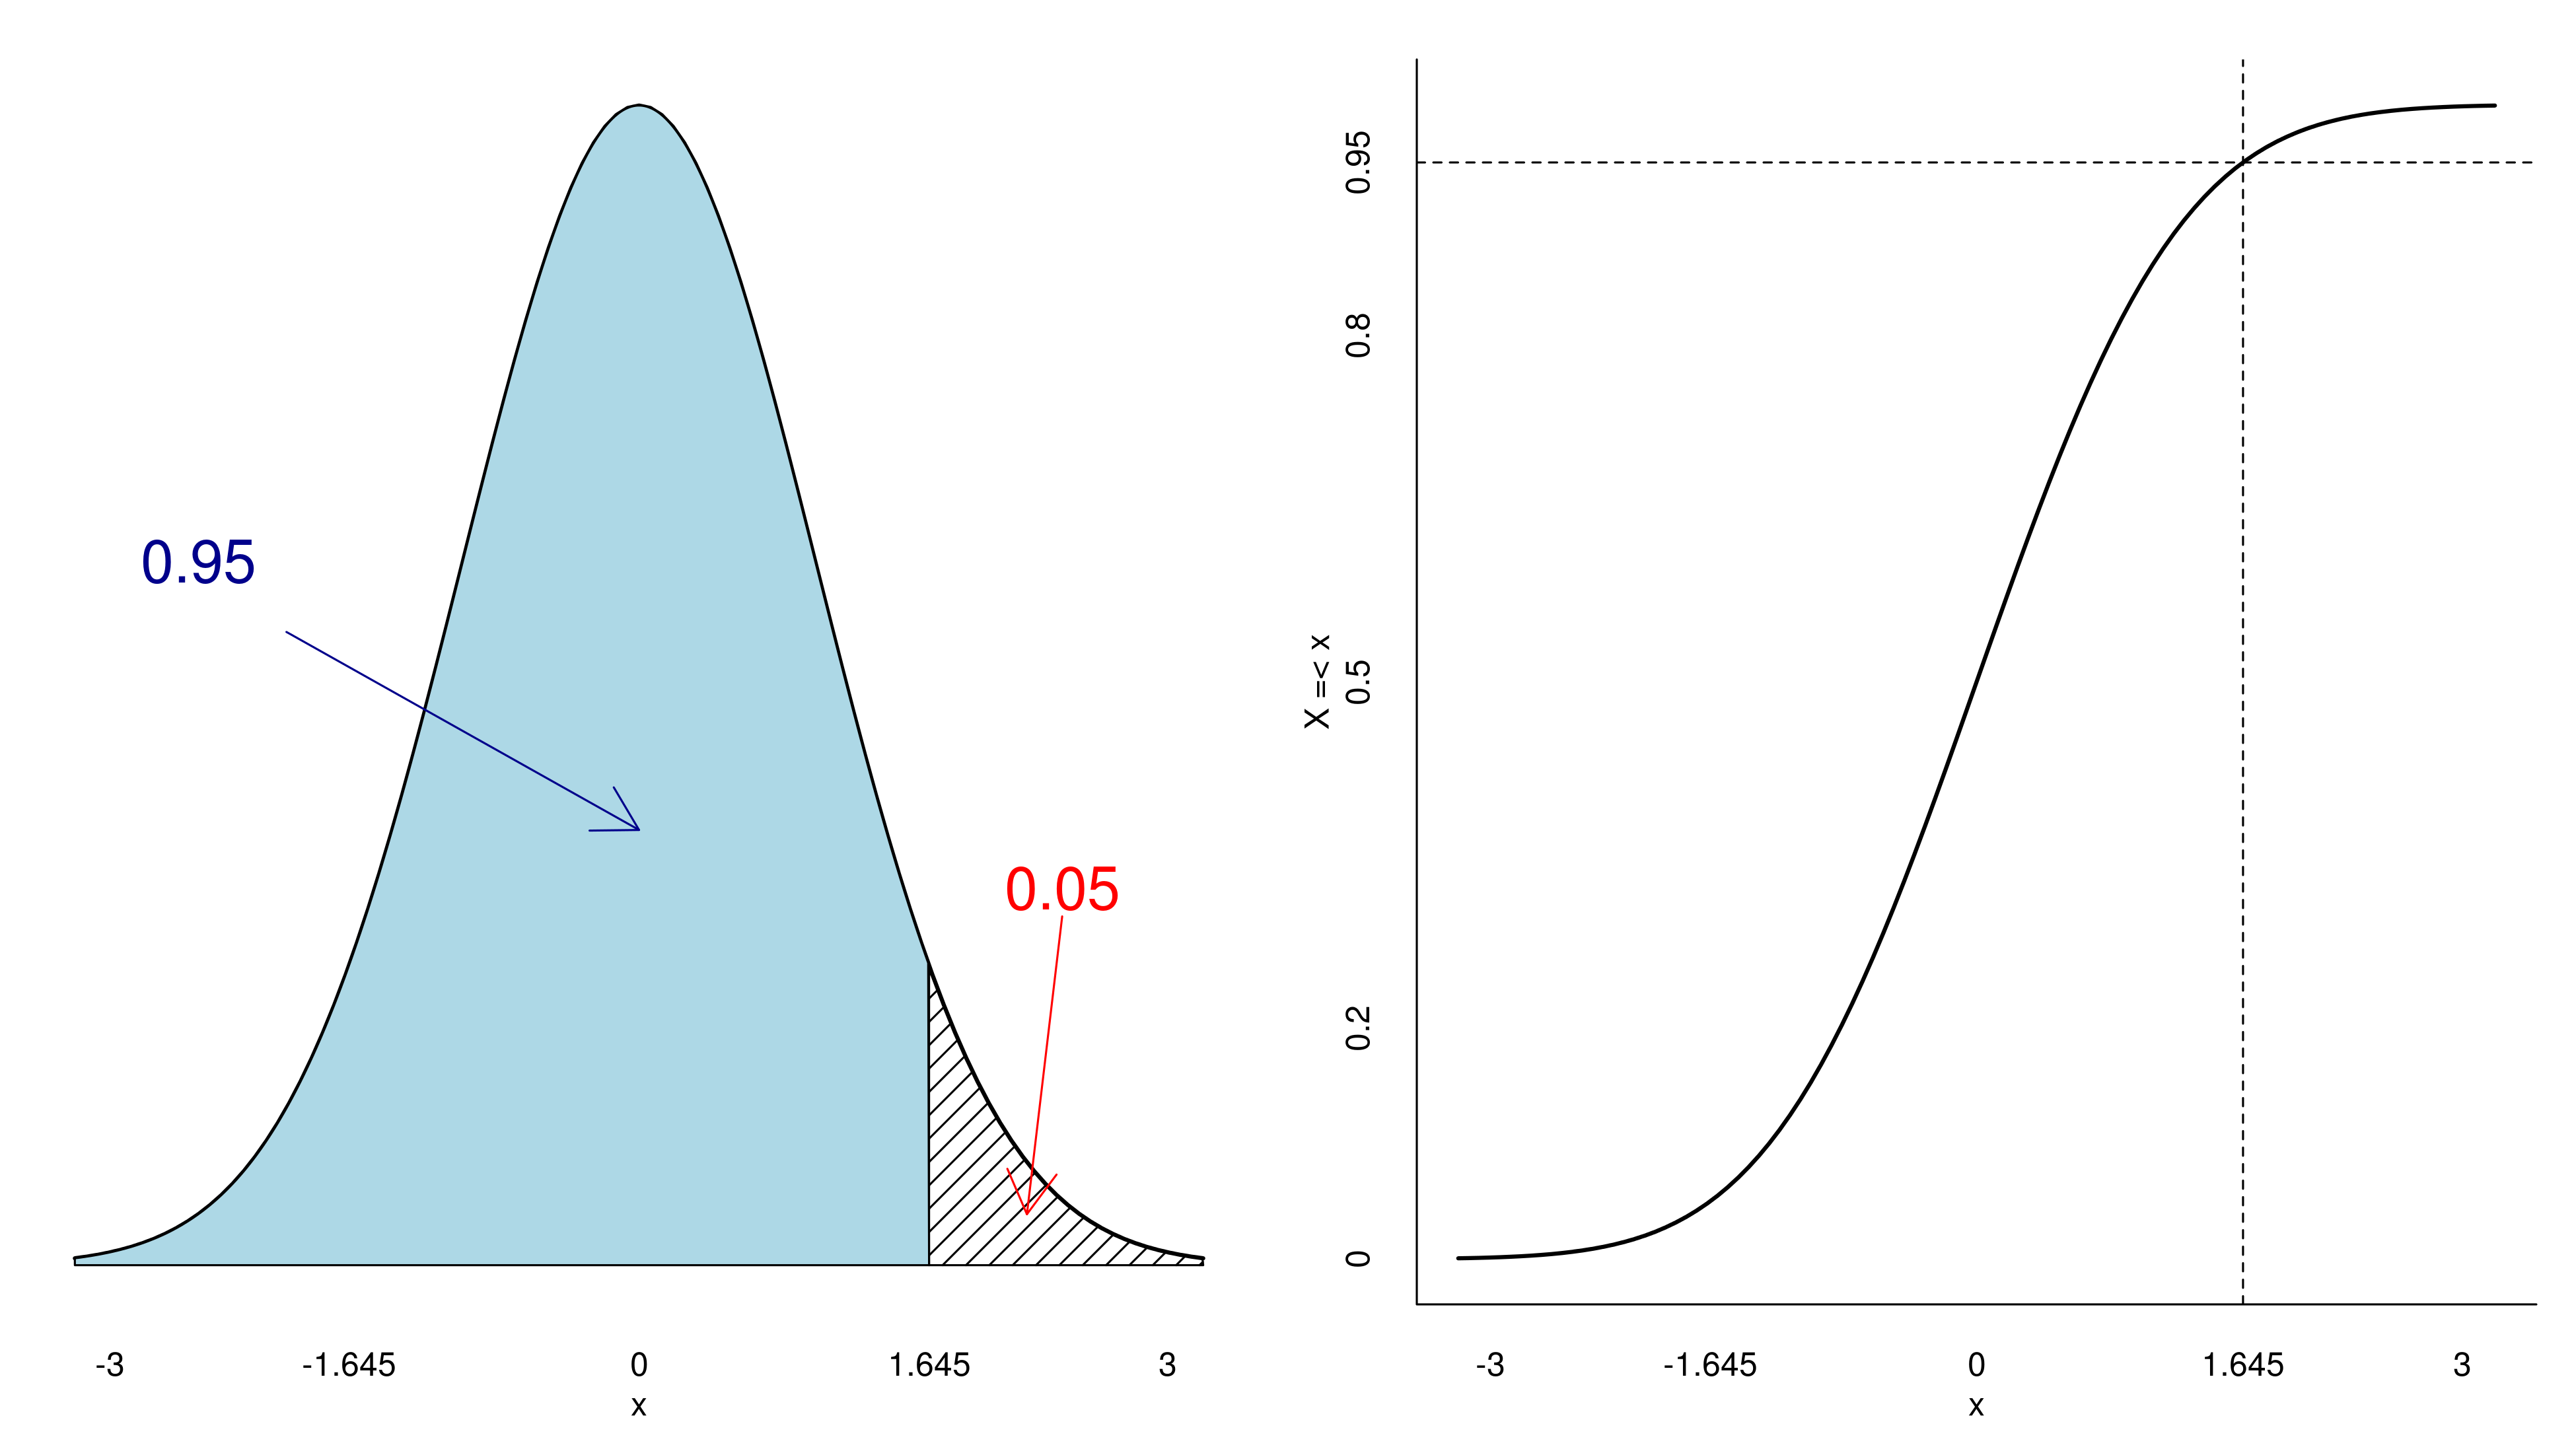
\includegraphics[width=0.7\linewidth]{figs/tables_NormCDF} 

}

\caption{The probability distribution function and the cumulative distribution function of the standard normal distribution N(0,1). The value of the 95\% quantile $q_{0.95} = 1.645$ is shown.}\label{fig:ncdf}
\end{figure}

\newpage

\begin{center}
\begin{tabular}{rr@{\ }r@{\ }r@{\ }r@{\ }r@{\ }r@{\ }r@{\ }r@{\ }r@{\ }r@{\ }r}
\multicolumn{11}{c}{NORMAL CUMULATIVE DISTRIBUTION FUNCTION}\\
\ \\
$x$&0.00&0.01&0.02&0.03&0.04&0.05&0.06&0.07&0.08&0.09\\
\ \\
0.0&0.5000&0.5040&0.5080&0.5120&0.5160&0.5199&0.5239&0.5279&0.5319&0.5359\\
0.1&0.5398&0.5438&0.5478&0.5517&0.5557&0.5596&0.5636&0.5675&0.5714&0.5753\\
0.2&0.5793&0.5832&0.5871&0.5910&0.5948&0.5987&0.6026&0.6064&0.6103&0.6141\\
0.3&0.6179&0.6217&0.6255&0.6293&0.6331&0.6368&0.6406&0.6443&0.6480&0.6517\\
0.4&0.6554&0.6591&0.6628&0.6664&0.6700&0.6736&0.6772&0.6808&0.6844&0.6879\\
0.5&0.6915&0.6950&0.6985&0.7019&0.7054&0.7088&0.7123&0.7157&0.7190&0.7224\\
0.6&0.7257&0.7291&0.7324&0.7357&0.7389&0.7422&0.7454&0.7486&0.7517&0.7549\\
0.7&0.7580&0.7611&0.7642&0.7673&0.7703&0.7734&0.7764&0.7794&0.7823&0.7852\\
0.8&0.7881&0.7910&0.7939&0.7967&0.7995&0.8023&0.8051&0.8078&0.8106&0.8133\\
0.9&0.8159&0.8186&0.8212&0.8238&0.8264&0.8289&0.8315&0.8340&0.8365&0.8389\\
1.0&0.8413&0.8438&0.8461&0.8485&0.8508&0.8531&0.8554&0.8577&0.8599&0.8621\\
1.1&0.8643&0.8665&0.8686&0.8708&0.8729&0.8749&0.8770&0.8790&0.8810&0.8830\\
1.2&0.8849&0.8869&0.8888&0.8907&0.8925&0.8944&0.8962&0.8980&0.8997&0.9015\\
1.3&0.9032&0.9049&0.9066&0.9082&0.9099&0.9115&0.9131&0.9147&0.9162&0.9177\\
1.4&0.9192&0.9207&0.9222&0.9236&0.9251&0.9265&0.9279&0.9292&0.9306&0.9319\\
1.5&0.9332&0.9345&0.9357&0.9370&0.9382&0.9394&0.9406&0.9418&0.9429&0.9441\\
1.6&0.9452&0.9463&0.9474&0.9484&0.9495&0.9505&0.9515&0.9525&0.9535&0.9545\\
1.7&0.9554&0.9564&0.9573&0.9582&0.9591&0.9599&0.9608&0.9616&0.9625&0.9633\\
1.8&0.9641&0.9649&0.9656&0.9664&0.9671&0.9678&0.9686&0.9693&0.9699&0.9706\\
1.9&0.9713&0.9719&0.9726&0.9732&0.9738&0.9744&0.9750&0.9756&0.9761&0.9767\\
2.0&0.9772&0.9778&0.9783&0.9788&0.9793&0.9798&0.9803&0.9808&0.9812&0.9817\\
2.1&0.9821&0.9826&0.9830&0.9834&0.9838&0.9842&0.9846&0.9850&0.9854&0.9857\\
2.2&0.9861&0.9864&0.9868&0.9871&0.9875&0.9878&0.9881&0.9884&0.9887&0.9890\\
2.3&0.9893&0.9896&0.9898&0.9901&0.9904&0.9906&0.9909&0.9911&0.9913&0.9916\\
2.4&0.9918&0.9920&0.9922&0.9925&0.9927&0.9929&0.9931&0.9932&0.9934&0.9936\\
2.5&0.9938&0.9940&0.9941&0.9943&0.9945&0.9946&0.9948&0.9949&0.9951&0.9952\\
2.6&0.9953&0.9955&0.9956&0.9957&0.9959&0.9960&0.9961&0.9962&0.9963&0.9964\\
2.7&0.9965&0.9966&0.9967&0.9968&0.9969&0.9970&0.9971&0.9972&0.9973&0.9974\\
2.8&0.9974&0.9975&0.9976&0.9977&0.9977&0.9978&0.9979&0.9979&0.9980&0.9981\\
2.9&0.9981&0.9982&0.9982&0.9983&0.9984&0.9984&0.9985&0.9985&0.9986&0.9986\\
3.0&0.9987&0.9987&0.9987&0.9988&0.9988&0.9989&0.9989&0.9989&0.9990&0.9990\\
3.1&0.9990&0.9991&0.9991&0.9991&0.9992&0.9992&0.9992&0.9992&0.9993&0.9993\\
3.2&0.9993&0.9993&0.9994&0.9994&0.9994&0.9994&0.9994&0.9995&0.9995&0.9995\\
3.3&0.9995&0.9995&0.9995&0.9996&0.9996&0.9996&0.9996&0.9996&0.9996&0.9997\\
3.4&0.9997&0.9997&0.9997&0.9997&0.9997&0.9997&0.9997&0.9997&0.9997&0.9998\\
3.5&0.9998&0.9998&0.9998&0.9998&0.9998&0.9998&0.9998&0.9998&0.9998&0.9998\\
3.6&0.9998&0.9998&0.9999&0.9999&0.9999&0.9999&0.9999&0.9999&0.9999&0.9999\\
3.7&0.9999&0.9999&0.9999&0.9999&0.9999&0.9999&0.9999&0.9999&0.9999&0.9999\\
3.8&0.9999&0.9999&0.9999&0.9999&0.9999&0.9999&0.9999&0.9999&0.9999&0.9999\\
3.9&1.0000&1.0000&1.0000&1.0000&1.0000&1.0000&1.0000&1.0000&1.0000&1.0000\\
\end{tabular}
\end{center}

\newpage

\begin{center}
\begin{tabular}
      {r@{\quad}r@{\,}r@{\,}r@{\,}r@{\,}r@{\,}r@{\,}r@{\,}r@{\,}r@{\,}r@{\,}r}
\multicolumn{12}{c}{QUANTILES OF THE STUDENT'S $t$ ($T_{\nu}$) DISTRIBUTION} \\
\ \\
$\nu$&.60&.667&.750&.800&.875&.900&.950&.975&.990&.995&.999 \\
\ \\
 1&0.325&0.577&1.000&1.376&2.414&3.078&6.314&12.706&31.821&63.657&318.31 \\
 2&0.289&0.500&0.816&1.061&1.604&1.886&2.920&4.303&6.965&9.925&22.327 \\
 3&0.277&0.476&0.765&0.978&1.423&1.638&2.353&3.182&4.541&5.841&10.215 \\
 4&0.271&0.464&0.741&0.941&1.344&1.533&2.132&2.776&3.747&4.604&7.173 \\
 5&0.267&0.457&0.727&0.920&1.301&1.476&2.015&2.571&3.365&4.032&5.893 \\
 6&0.265&0.453&0.718&0.906&1.273&1.440&1.943&2.447&3.143&3.707&5.208 \\
 7&0.263&0.449&0.711&0.896&1.254&1.415&1.895&2.365&2.998&3.499&4.785 \\
 8&0.262&0.447&0.706&0.889&1.240&1.397&1.860&2.306&2.896&3.355&4.501 \\
 9&0.261&0.445&0.703&0.883&1.230&1.383&1.833&2.262&2.821&3.250&4.297 \\
10&0.260&0.444&0.700&0.879&1.221&1.372&1.812&2.228&2.764&3.169&4.144 \\
11&0.260&0.443&0.697&0.876&1.214&1.363&1.796&2.201&2.718&3.106&4.025 \\
12&0.259&0.442&0.695&0.873&1.209&1.356&1.782&2.179&2.681&3.055&3.930 \\
13&0.259&0.441&0.694&0.870&1.204&1.350&1.771&2.160&2.650&3.012&3.852 \\
14&0.258&0.440&0.692&0.868&1.200&1.345&1.761&2.145&2.624&2.977&3.787 \\
15&0.258&0.439&0.691&0.866&1.197&1.341&1.753&2.131&2.602&2.947&3.733 \\
16&0.258&0.439&0.690&0.865&1.194&1.337&1.746&2.120&2.583&2.921&3.686 \\
17&0.257&0.438&0.689&0.863&1.191&1.333&1.740&2.110&2.567&2.898&3.646 \\
18&0.257&0.438&0.688&0.862&1.189&1.330&1.734&2.101&2.552&2.878&3.610 \\
19&0.257&0.438&0.688&0.861&1.187&1.328&1.729&2.093&2.539&2.861&3.579 \\
20&0.257&0.437&0.687&0.860&1.185&1.325&1.725&2.086&2.528&2.845&3.552 \\
21&0.257&0.437&0.686&0.859&1.183&1.323&1.721&2.080&2.518&2.831&3.527 \\
22&0.256&0.437&0.686&0.858&1.182&1.321&1.717&2.074&2.508&2.819&3.505 \\
23&0.256&0.436&0.685&0.858&1.180&1.319&1.714&2.069&2.500&2.807&3.485 \\
24&0.256&0.436&0.685&0.857&1.179&1.318&1.711&2.064&2.492&2.797&3.467 \\
25&0.256&0.436&0.684&0.856&1.178&1.316&1.708&2.060&2.485&2.787&3.450 \\
26&0.256&0.436&0.684&0.856&1.177&1.315&1.706&2.056&2.479&2.779&3.435 \\
27&0.256&0.435&0.684&0.855&1.176&1.314&1.703&2.052&2.473&2.771&3.421 \\
28&0.256&0.435&0.683&0.855&1.175&1.313&1.701&2.048&2.467&2.763&3.408 \\
29&0.256&0.435&0.683&0.854&1.174&1.311&1.699&2.045&2.462&2.756&3.396 \\
30&0.256&0.435&0.683&0.854&1.173&1.310&1.697&2.042&2.457&2.750&3.385 \\
35&0.255&0.434&0.682&0.852&1.170&1.306&1.690&2.030&2.438&2.724&3.340 \\
40&0.255&0.434&0.681&0.851&1.167&1.303&1.684&2.021&2.423&2.704&3.307 \\
45&0.255&0.434&0.680&0.850&1.165&1.301&1.679&2.014&2.412&2.690&3.281 \\
50&0.255&0.433&0.679&0.849&1.164&1.299&1.676&2.009&2.403&2.678&3.261 \\
55&0.255&0.433&0.679&0.848&1.163&1.297&1.673&2.004&2.396&2.668&3.245 \\
60&0.254&0.433&0.679&0.848&1.162&1.296&1.671&2.000&2.390&2.660&3.232 \\
$\infty$
  &0.253&0.431&0.674&0.842&1.150&1.282&1.645&1.960&2.326&2.576&3.090
\end{tabular}
\end{center}

\newpage

\begin{center}
\begin{tabular}{rr@{\ }r@{\ }r@{\ }r@{\ }r@{\ }r@{\ }r@{\ }r@{\ }r@{\ }r@{\ }r}
& &\multicolumn{10}{c}{QUANTILES OF THE $F(\nu_1, \nu_2)$ DISTRIBUTION}\\
\ \\
$\nu_2 \backslash  \nu_1$ & & 1 & 2 & 3 & 4 & 5 & 6 & 7 & 8 & 9 & 10\\
 & \textit{q}  &  &  &  &  &  &  &  &  & & \\
\rule{0pt}{2.5ex} & 0.9 & 39.86 & 49.50 & 53.59 & 55.83 & 57.24 & 58.20 & 58.91 & 59.44 & 59.86 & 60.19\\
 & 0.95 & 161.45 & 199.50 & 215.71 & 224.58 & 230.16 & 233.99 & 236.77 & 238.88 & 240.54 & 241.88\\
1 & 0.975 & 647.79 & 799.50 & 864.16 & 899.58 & 921.85 & 937.11 & 948.22 & 956.66 & 963.28 & 968.63\\
 & 0.99 &   &  &   &  &  &  &   &  &  &\\
 & 0.999 &  &  &   &  &  &  &   &  &  &\\
\rule{0pt}{2.5ex} & 0.9 & 8.53 & 9.00 & 9.16 & 9.24 & 9.29 & 9.33 & 9.35 & 9.37 & 9.38 & 9.39\\
 & 0.95 & 18.51 & 19.00 & 19.16 & 19.25 & 19.30 & 19.33 & 19.35 & 19.37 & 19.38 & 19.40\\
2 & 0.975 & 38.51 & 39.00 & 39.17 & 39.25 & 39.30 & 39.33 & 39.36 & 39.37 & 39.39 & 39.40\\
 & 0.99 & 98.50 & 99.00 & 99.17 & 99.25 & 99.30 & 99.33 & 99.36 & 99.37 & 99.39 & 99.40\\
 & 0.999 & 998.50 & 999.00 & 999.17 & 999.25 & 999.30 & 999.33 & 999.36 & 999.37 & 999.39 & 999.40\\
\rule{0pt}{2.5ex} & 0.9 & 5.54 & 5.46 & 5.39 & 5.34 & 5.31 & 5.28 & 5.27 & 5.25 & 5.24 & 5.23\\
 & 0.95 & 10.13 & 9.55 & 9.28 & 9.12 & 9.01 & 8.94 & 8.89 & 8.85 & 8.81 & 8.79\\
3 & 0.975 & 17.44 & 16.04 & 15.44 & 15.10 & 14.88 & 14.73 & 14.62 & 14.54 & 14.47 & 14.42\\
 & 0.99 & 34.12 & 30.82 & 29.46 & 28.71 & 28.24 & 27.91 & 27.67 & 27.49 & 27.35 & 27.23\\
 & 0.999 & 167.03 & 148.50 & 141.11 & 137.10 & 134.58 & 132.85 & 131.58 & 130.62 & 129.86 & 129.25\\
\rule{0pt}{2.5ex} & 0.9 & 4.54 & 4.32 & 4.19 & 4.11 & 4.05 & 4.01 & 3.98 & 3.95 & 3.94 & 3.92\\
 & 0.95 & 7.71 & 6.94 & 6.59 & 6.39 & 6.26 & 6.16 & 6.09 & 6.04 & 6.00 & 5.96\\
4 & 0.975 & 12.22 & 10.65 & 9.98 & 9.60 & 9.36 & 9.20 & 9.07 & 8.98 & 8.90 & 8.84\\
 & 0.99 & 21.20 & 18.00 & 16.69 & 15.98 & 15.52 & 15.21 & 14.98 & 14.80 & 14.66 & 14.55\\
 & 0.999 & 74.14 & 61.25 & 56.18 & 53.44 & 51.71 & 50.53 & 49.66 & 49.00 & 48.47 & 48.05\\
\rule{0pt}{2.5ex} & 0.9 & 4.06 & 3.78 & 3.62 & 3.52 & 3.45 & 3.40 & 3.37 & 3.34 & 3.32 & 3.30\\
 & 0.95 & 6.61 & 5.79 & 5.41 & 5.19 & 5.05 & 4.95 & 4.88 & 4.82 & 4.77 & 4.74\\
5 & 0.975 & 10.01 & 8.43 & 7.76 & 7.39 & 7.15 & 6.98 & 6.85 & 6.76 & 6.68 & 6.62\\
 & 0.99 & 16.26 & 13.27 & 12.06 & 11.39 & 10.97 & 10.67 & 10.46 & 10.29 & 10.16 & 10.05\\
 & 0.999 & 47.18 & 37.12 & 33.20 & 31.09 & 29.75 & 28.83 & 28.16 & 27.65 & 27.24 & 26.92\\
\rule{0pt}{2.5ex} & 0.9 & 3.78 & 3.46 & 3.29 & 3.18 & 3.11 & 3.05 & 3.01 & 2.98 & 2.96 & 2.94\\
 & 0.95 & 5.99 & 5.14 & 4.76 & 4.53 & 4.39 & 4.28 & 4.21 & 4.15 & 4.10 & 4.06\\
6 & 0.975 & 8.81 & 7.26 & 6.60 & 6.23 & 5.99 & 5.82 & 5.70 & 5.60 & 5.52 & 5.46\\
 & 0.99 & 13.75 & 10.92 & 9.78 & 9.15 & 8.75 & 8.47 & 8.26 & 8.10 & 7.98 & 7.87\\
 & 0.999 & 35.51 & 27.00 & 23.70 & 21.92 & 20.80 & 20.03 & 19.46 & 19.03 & 18.69 & 18.41\\
\rule{0pt}{2.5ex} & 0.9 & 3.59 & 3.26 & 3.07 & 2.96 & 2.88 & 2.83 & 2.78 & 2.75 & 2.72 & 2.70\\
 & 0.95 & 5.59 & 4.74 & 4.35 & 4.12 & 3.97 & 3.87 & 3.79 & 3.73 & 3.68 & 3.64\\
7 & 0.975 & 8.07 & 6.54 & 5.89 & 5.52 & 5.29 & 5.12 & 4.99 & 4.90 & 4.82 & 4.76\\
 & 0.99 & 12.25 & 9.55 & 8.45 & 7.85 & 7.46 & 7.19 & 6.99 & 6.84 & 6.72 & 6.62\\
 & 0.999 & 29.25 & 21.69 & 18.77 & 17.20 & 16.21 & 15.52 & 15.02 & 14.63 & 14.33 & 14.08\\
\rule{0pt}{2.5ex} & 0.9 & 3.46 & 3.11 & 2.92 & 2.81 & 2.73 & 2.67 & 2.62 & 2.59 & 2.56 & 2.54\\
 & 0.95 & 5.32 & 4.46 & 4.07 & 3.84 & 3.69 & 3.58 & 3.50 & 3.44 & 3.39 & 3.35\\
8 & 0.975 & 7.57 & 6.06 & 5.42 & 5.05 & 4.82 & 4.65 & 4.53 & 4.43 & 4.36 & 4.30\\
 & 0.99 & 11.26 & 8.65 & 7.59 & 7.01 & 6.63 & 6.37 & 6.18 & 6.03 & 5.91 & 5.81\\
 & 0.999 & 25.41 & 18.49 & 15.83 & 14.39 & 13.48 & 12.86 & 12.40 & 12.05 & 11.77 & 11.54\\
\end{tabular}
\end{center}

\newpage

\begin{center}
\begin{tabular}{rr@{\ \ }r@{\ \ }r@{\ \ }r@{\ \ }r@{\ \ }r@{\ \ }r@{\ \ }r@{\ \ }r@{\ \ }r@{\ \ }r@{ }}
& &\multicolumn{10}{c}{QUANTILES OF THE $F(\nu_1, \nu_2)$ DISTRIBUTION}\\
\ \\
$\nu_2\backslash\nu_1$ & & 1 & 2 & 3 & 4 & 5 & 6 & 7 & 8 & 9 & 10\\
 & \textit{q}  &  &  &  &  &  &  &  &  & & \\
\rule{0pt}{2.5ex} & 0.9 & 3.36 & 3.01 & 2.81 & 2.69 & 2.61 & 2.55 & 2.51 & 2.47 & 2.44 & 2.42\\
 & 0.95 & 5.12 & 4.26 & 3.86 & 3.63 & 3.48 & 3.37 & 3.29 & 3.23 & 3.18 & 3.14\\
9 & 0.975 & 7.21 & 5.71 & 5.08 & 4.72 & 4.48 & 4.32 & 4.20 & 4.10 & 4.03 & 3.96\\
 & 0.99 & 10.56 & 8.02 & 6.99 & 6.42 & 6.06 & 5.80 & 5.61 & 5.47 & 5.35 & 5.26\\
 & 0.999 & 22.86 & 16.39 & 13.90 & 12.56 & 11.71 & 11.13 & 10.70 & 10.37 & 10.11 & 9.89\\
\rule{0pt}{2.5ex} & 0.9 & 3.29 & 2.92 & 2.73 & 2.61 & 2.52 & 2.46 & 2.41 & 2.38 & 2.35 & 2.32\\
 & 0.95 & 4.96 & 4.10 & 3.71 & 3.48 & 3.33 & 3.22 & 3.14 & 3.07 & 3.02 & 2.98\\
10 & 0.975 & 6.94 & 5.46 & 4.83 & 4.47 & 4.24 & 4.07 & 3.95 & 3.85 & 3.78 & 3.72\\
 & 0.99 & 10.04 & 7.56 & 6.55 & 5.99 & 5.64 & 5.39 & 5.20 & 5.06 & 4.94 & 4.85\\
 & 0.999 & 21.04 & 14.91 & 12.55 & 11.28 & 10.48 & 9.93 & 9.52 & 9.20 & 8.96 & 8.75\\
\rule{0pt}{2.5ex} & 0.9 & 3.23 & 2.86 & 2.66 & 2.54 & 2.45 & 2.39 & 2.34 & 2.30 & 2.27 & 2.25\\
 & 0.95 & 4.84 & 3.98 & 3.59 & 3.36 & 3.20 & 3.09 & 3.01 & 2.95 & 2.90 & 2.85\\
11 & 0.975 & 6.72 & 5.26 & 4.63 & 4.28 & 4.04 & 3.88 & 3.76 & 3.66 & 3.59 & 3.53\\
 & 0.99 & 9.65 & 7.21 & 6.22 & 5.67 & 5.32 & 5.07 & 4.89 & 4.74 & 4.63 & 4.54\\
 & 0.999 & 19.69 & 13.81 & 11.56 & 10.35 & 9.58 & 9.05 & 8.66 & 8.35 & 8.12 & 7.92\\
\rule{0pt}{2.5ex} & 0.9 & 3.18 & 2.81 & 2.61 & 2.48 & 2.39 & 2.33 & 2.28 & 2.24 & 2.21 & 2.19\\
 & 0.95 & 4.75 & 3.89 & 3.49 & 3.26 & 3.11 & 3.00 & 2.91 & 2.85 & 2.80 & 2.75\\
12 & 0.975 & 6.55 & 5.10 & 4.47 & 4.12 & 3.89 & 3.73 & 3.61 & 3.51 & 3.44 & 3.37\\
 & 0.99 & 9.33 & 6.93 & 5.95 & 5.41 & 5.06 & 4.82 & 4.64 & 4.50 & 4.39 & 4.30\\
 & 0.999 & 18.64 & 12.97 & 10.80 & 9.63 & 8.89 & 8.38 & 8.00 & 7.71 & 7.48 & 7.29\\
\rule{0pt}{2.5ex} & 0.9 & 3.14 & 2.76 & 2.56 & 2.43 & 2.35 & 2.28 & 2.23 & 2.20 & 2.16 & 2.14\\
 & 0.95 & 4.67 & 3.81 & 3.41 & 3.18 & 3.03 & 2.92 & 2.83 & 2.77 & 2.71 & 2.67\\
13 & 0.975 & 6.41 & 4.97 & 4.35 & 4.00 & 3.77 & 3.60 & 3.48 & 3.39 & 3.31 & 3.25\\
 & 0.99 & 9.07 & 6.70 & 5.74 & 5.21 & 4.86 & 4.62 & 4.44 & 4.30 & 4.19 & 4.10\\
 & 0.999 & 17.82 & 12.31 & 10.21 & 9.07 & 8.35 & 7.86 & 7.49 & 7.21 & 6.98 & 6.80\\
\rule{0pt}{2.5ex} & 0.9 & 3.10 & 2.73 & 2.52 & 2.39 & 2.31 & 2.24 & 2.19 & 2.15 & 2.12 & 2.10\\
 & 0.95 & 4.60 & 3.74 & 3.34 & 3.11 & 2.96 & 2.85 & 2.76 & 2.70 & 2.65 & 2.60\\
14 & 0.975 & 6.30 & 4.86 & 4.24 & 3.89 & 3.66 & 3.50 & 3.38 & 3.29 & 3.21 & 3.15\\
 & 0.99 & 8.86 & 6.51 & 5.56 & 5.04 & 4.69 & 4.46 & 4.28 & 4.14 & 4.03 & 3.94\\
 & 0.999 & 17.14 & 11.78 & 9.73 & 8.62 & 7.92 & 7.44 & 7.08 & 6.80 & 6.58 & 6.40\\
\rule{0pt}{2.5ex} & 0.9 & 3.07 & 2.70 & 2.49 & 2.36 & 2.27 & 2.21 & 2.16 & 2.12 & 2.09 & 2.06\\
 & 0.95 & 4.54 & 3.68 & 3.29 & 3.06 & 2.90 & 2.79 & 2.71 & 2.64 & 2.59 & 2.54\\
15 & 0.975 & 6.20 & 4.77 & 4.15 & 3.80 & 3.58 & 3.41 & 3.29 & 3.20 & 3.12 & 3.06\\
 & 0.99 & 8.68 & 6.36 & 5.42 & 4.89 & 4.56 & 4.32 & 4.14 & 4.00 & 3.89 & 3.80\\
 & 0.999 & 16.59 & 11.34 & 9.34 & 8.25 & 7.57 & 7.09 & 6.74 & 6.47 & 6.26 & 6.08\\
\rule{0pt}{2.5ex} & 0.9 & 3.05 & 2.67 & 2.46 & 2.33 & 2.24 & 2.18 & 2.13 & 2.09 & 2.06 & 2.03\\
 & 0.95 & 4.49 & 3.63 & 3.24 & 3.01 & 2.85 & 2.74 & 2.66 & 2.59 & 2.54 & 2.49\\
16 & 0.975 & 6.12 & 4.69 & 4.08 & 3.73 & 3.50 & 3.34 & 3.22 & 3.12 & 3.05 & 2.99\\
 & 0.99 & 8.53 & 6.23 & 5.29 & 4.77 & 4.44 & 4.20 & 4.03 & 3.89 & 3.78 & 3.69\\
 & 0.999 & 16.12 & 10.97 & 9.01 & 7.94 & 7.27 & 6.80 & 6.46 & 6.19 & 5.98 & 5.81\\
\end{tabular}
\end{center}

\newpage

\begin{center}
\begin{tabular}{rr@{\ \ }r@{\ \ }r@{\ \ }r@{\ \ }r@{\ \ }r@{\ \ }r@{\ \ }r@{\ \ }r@{\ \ }r@{\ \ }r@{ }}
& &\multicolumn{10}{c}{QUANTILES OF THE $F(\nu_1, \nu_2)$ DISTRIBUTION}\\
\ \\
$\nu_2\backslash\nu_1$ & & 1 & 2 & 3 & 4 & 5 & 6 & 7 & 8 & 9 & 10\\
 & \textit{q}  &  &  &  &  &  &  &  &  & & \\
\rule{0pt}{2.5ex} & 0.9 & 3.03 & 2.64 & 2.44 & 2.31 & 2.22 & 2.15 & 2.10 & 2.06 & 2.03 & 2.00\\
 & 0.95 & 4.45 & 3.59 & 3.20 & 2.96 & 2.81 & 2.70 & 2.61 & 2.55 & 2.49 & 2.45\\
17 & 0.975 & 6.04 & 4.62 & 4.01 & 3.66 & 3.44 & 3.28 & 3.16 & 3.06 & 2.98 & 2.92\\
 & 0.99 & 8.40 & 6.11 & 5.18 & 4.67 & 4.34 & 4.10 & 3.93 & 3.79 & 3.68 & 3.59\\
 & 0.999 & 15.72 & 10.66 & 8.73 & 7.68 & 7.02 & 6.56 & 6.22 & 5.96 & 5.75 & 5.58\\
\rule{0pt}{2.5ex} & 0.9 & 3.01 & 2.62 & 2.42 & 2.29 & 2.20 & 2.13 & 2.08 & 2.04 & 2.00 & 1.98\\
 & 0.95 & 4.41 & 3.55 & 3.16 & 2.93 & 2.77 & 2.66 & 2.58 & 2.51 & 2.46 & 2.41\\
18 & 0.975 & 5.98 & 4.56 & 3.95 & 3.61 & 3.38 & 3.22 & 3.10 & 3.01 & 2.93 & 2.87\\
 & 0.99 & 8.29 & 6.01 & 5.09 & 4.58 & 4.25 & 4.01 & 3.84 & 3.71 & 3.60 & 3.51\\
 & 0.999 & 15.38 & 10.39 & 8.49 & 7.46 & 6.81 & 6.35 & 6.02 & 5.76 & 5.56 & 5.39\\
\rule{0pt}{2.5ex} & 0.9 & 2.97 & 2.59 & 2.38 & 2.25 & 2.16 & 2.09 & 2.04 & 2.00 & 1.96 & 1.94\\
 & 0.95 & 4.35 & 3.49 & 3.10 & 2.87 & 2.71 & 2.60 & 2.51 & 2.45 & 2.39 & 2.35\\
20 & 0.975 & 5.87 & 4.46 & 3.86 & 3.51 & 3.29 & 3.13 & 3.01 & 2.91 & 2.84 & 2.77\\
 & 0.99 & 8.10 & 5.85 & 4.94 & 4.43 & 4.10 & 3.87 & 3.70 & 3.56 & 3.46 & 3.37\\
 & 0.999 & 14.82 & 9.95 & 8.10 & 7.10 & 6.46 & 6.02 & 5.69 & 5.44 & 5.24 & 5.08\\
\rule{0pt}{2.5ex} & 0.9 & 2.92 & 2.53 & 2.32 & 2.18 & 2.09 & 2.02 & 1.97 & 1.93 & 1.89 & 1.87\\
 & 0.95 & 4.24 & 3.39 & 2.99 & 2.76 & 2.60 & 2.49 & 2.40 & 2.34 & 2.28 & 2.24\\
25 & 0.975 & 5.69 & 4.29 & 3.69 & 3.35 & 3.13 & 2.97 & 2.85 & 2.75 & 2.68 & 2.61\\
 & 0.99 & 7.77 & 5.57 & 4.68 & 4.18 & 3.85 & 3.63 & 3.46 & 3.32 & 3.22 & 3.13\\
 & 0.999 & 13.88 & 9.22 & 7.45 & 6.49 & 5.89 & 5.46 & 5.15 & 4.91 & 4.71 & 4.56\\
\rule{0pt}{2.5ex} & 0.9 & 2.88 & 2.49 & 2.28 & 2.14 & 2.05 & 1.98 & 1.93 & 1.88 & 1.85 & 1.82\\
 & 0.95 & 4.17 & 3.32 & 2.92 & 2.69 & 2.53 & 2.42 & 2.33 & 2.27 & 2.21 & 2.16\\
30 & 0.975 & 5.57 & 4.18 & 3.59 & 3.25 & 3.03 & 2.87 & 2.75 & 2.65 & 2.57 & 2.51\\
 & 0.99 & 7.56 & 5.39 & 4.51 & 4.02 & 3.70 & 3.47 & 3.30 & 3.17 & 3.07 & 2.98\\
 & 0.999 & 13.29 & 8.77 & 7.05 & 6.12 & 5.53 & 5.12 & 4.82 & 4.58 & 4.39 & 4.24\\
\rule{0pt}{2.5ex} & 0.9 & 2.84 & 2.44 & 2.23 & 2.09 & 2.00 & 1.93 & 1.87 & 1.83 & 1.79 & 1.76\\
 & 0.95 & 4.08 & 3.23 & 2.84 & 2.61 & 2.45 & 2.34 & 2.25 & 2.18 & 2.12 & 2.08\\
40 & 0.975 & 5.42 & 4.05 & 3.46 & 3.13 & 2.90 & 2.74 & 2.62 & 2.53 & 2.45 & 2.39\\
 & 0.99 & 7.31 & 5.18 & 4.31 & 3.83 & 3.51 & 3.29 & 3.12 & 2.99 & 2.89 & 2.80\\
 & 0.999 & 12.61 & 8.25 & 6.59 & 5.70 & 5.13 & 4.73 & 4.44 & 4.21 & 4.02 & 3.87\\
\rule{0pt}{2.5ex} & 0.9 & 2.81 & 2.41 & 2.20 & 2.06 & 1.97 & 1.90 & 1.84 & 1.80 & 1.76 & 1.73\\
 & 0.95 & 4.03 & 3.18 & 2.79 & 2.56 & 2.40 & 2.29 & 2.20 & 2.13 & 2.07 & 2.03\\
50 & 0.975 & 5.34 & 3.97 & 3.39 & 3.05 & 2.83 & 2.67 & 2.55 & 2.46 & 2.38 & 2.32\\
 & 0.99 & 7.17 & 5.06 & 4.20 & 3.72 & 3.41 & 3.19 & 3.02 & 2.89 & 2.78 & 2.70\\
 & 0.999 & 12.22 & 7.96 & 6.34 & 5.46 & 4.90 & 4.51 & 4.22 & 4.00 & 3.82 & 3.67\\
\rule{0pt}{2.5ex} & 0.9 & 2.79 & 2.39 & 2.18 & 2.04 & 1.95 & 1.87 & 1.82 & 1.77 & 1.74 & 1.71\\
 & 0.95 & 4.00 & 3.15 & 2.76 & 2.53 & 2.37 & 2.25 & 2.17 & 2.10 & 2.04 & 1.99\\
60 & 0.975 & 5.29 & 3.93 & 3.34 & 3.01 & 2.79 & 2.63 & 2.51 & 2.41 & 2.33 & 2.27\\
 & 0.99 & 7.08 & 4.98 & 4.13 & 3.65 & 3.34 & 3.12 & 2.95 & 2.82 & 2.72 & 2.63\\
 & 0.999 & 11.97 & 7.77 & 6.17 & 5.31 & 4.76 & 4.37 & 4.09 & 3.86 & 3.69 & 3.54\\
\end{tabular}
\end{center}

\newpage

\begin{center}
\begin{tabular}{rr@{\ \ }r@{\ \ }r@{\ \ }r@{\ \ }r@{\ \ }r@{\ \ }r@{\ \ }r@{\ \ }r@{\ \ }r@{\ \ }r@{ }}
& &\multicolumn{10}{c}{QUANTILES OF THE $F(\nu_1, \nu_2)$ DISTRIBUTION}\\
\ \\
$\nu_2\backslash\nu_1$ & & 1 & 2 & 3 & 4 & 5 & 6 & 7 & 8 & 9 & 10\\
 & \textit{q}  &  &  &  &  &  &  &  &  & & \\
\rule{0pt}{2.5ex} & 0.9 & 2.77 & 2.37 & 2.15 & 2.02 & 1.92 & 1.85 & 1.79 & 1.75 & 1.71 & 1.68\\
 & 0.95 & 3.96 & 3.11 & 2.72 & 2.49 & 2.33 & 2.21 & 2.13 & 2.06 & 2.00 & 1.95\\
80 & 0.975 & 5.22 & 3.86 & 3.28 & 2.95 & 2.73 & 2.57 & 2.45 & 2.35 & 2.28 & 2.21\\
 & 0.99 & 6.96 & 4.88 & 4.04 & 3.56 & 3.26 & 3.04 & 2.87 & 2.74 & 2.64 & 2.55\\
 & 0.999 & 11.67 & 7.54 & 5.97 & 5.12 & 4.58 & 4.20 & 3.92 & 3.70 & 3.53 & 3.39\\
\rule{0pt}{2.5ex} & 0.9 & 2.74 & 2.34 & 2.12 & 1.98 & 1.89 & 1.81 & 1.76 & 1.71 & 1.67 & 1.64\\
 & 0.95 & 3.90 & 3.06 & 2.66 & 2.43 & 2.27 & 2.16 & 2.07 & 2.00 & 1.94 & 1.89\\
150 & 0.975 & 5.13 & 3.78 & 3.20 & 2.87 & 2.65 & 2.49 & 2.37 & 2.28 & 2.20 & 2.13\\
 & 0.99 & 6.81 & 4.75 & 3.91 & 3.45 & 3.14 & 2.92 & 2.76 & 2.63 & 2.53 & 2.44\\
 & 0.999 & 11.27 & 7.24 & 5.71 & 4.88 & 4.35 & 3.98 & 3.71 & 3.49 & 3.32 & 3.18\\
\rule{0pt}{2.5ex} & 0.9 & 2.73 & 2.33 & 2.11 & 1.97 & 1.88 & 1.80 & 1.75 & 1.70 & 1.66 & 1.63\\
 & 0.95 & 3.89 & 3.04 & 2.65 & 2.42 & 2.26 & 2.14 & 2.06 & 1.98 & 1.93 & 1.88\\
200 & 0.975 & 5.10 & 3.76 & 3.18 & 2.85 & 2.63 & 2.47 & 2.35 & 2.26 & 2.18 & 2.11\\
 & 0.99 & 6.76 & 4.71 & 3.88 & 3.41 & 3.11 & 2.89 & 2.73 & 2.60 & 2.50 & 2.41\\
 & 0.999 & 11.15 & 7.15 & 5.63 & 4.81 & 4.29 & 3.92 & 3.65 & 3.43 & 3.26 & 3.12\\
\end{tabular}
\end{center}

\newpage

\begin{center}
\begin{tabular}{rr@{\ }r@{\ }r@{\ }r@{\ }r@{\ }r@{\ }r@{\ }r@{\ }r@{\ }r@{\ }r}
& &\multicolumn{10}{c}{QUANTILES OF THE $F(\nu_l, \nu_2)$ DISTRIBUTION}\\
\ \\
 $\nu_2\backslash\nu_l$ & & 12 & 15 & 20 & 25 & 30 & 35 & 40 & 50 & 70 & 100\\
 & \textit{q}  &  &  &  &  &  &  &  &  & & \\
 \rule{0pt}{2.5ex} & 0.9 & 60.71 & 61.22 & 61.74 & 62.05 & 62.26 & 62.42 & 62.53 & 62.69 & 62.87 & 63.01\\
 & 0.95 & 243.91 & 245.95 & 248.01 & 249.26 & 250.10 & 250.69 & 251.14 & 251.77 & 252.50 & 253.04\\
1 & 0.975 & 976.71 & 984.87 & 993.10 & 998.08 &   &   &   &   &  &  \\
 & 0.99  &   &  &   &  &  &  &   &  &\\
 & 0.999  &   &  &   &  &  &  &   &  & \\
\rule{0pt}{2.5ex} & 0.9 & 9.41 & 9.42 & 9.44 & 9.45 & 9.46 & 9.46 & 9.47 & 9.47 & 9.48 & 9.48\\
 & 0.95 & 19.41 & 19.43 & 19.45 & 19.46 & 19.46 & 19.47 & 19.47 & 19.48 & 19.48 & 19.49\\
2 & 0.975 & 39.41 & 39.43 & 39.45 & 39.46 & 39.46 & 39.47 & 39.47 & 39.48 & 39.48 & 39.49\\
 & 0.99 & 99.42 & 99.43 & 99.45 & 99.46 & 99.47 & 99.47 & 99.47 & 99.48 & 99.48 & 99.49\\
 & 0.999 & 999.42 & 999.43 & 999.45 & 999.46 & 999.47 & 999.47 & 999.47 & 999.48 & 999.49 & 999.49\\
\rule{0pt}{2.5ex} & 0.9 & 5.22 & 5.20 & 5.18 & 5.17 & 5.17 & 5.16 & 5.16 & 5.15 & 5.15 & 5.14\\
 & 0.95 & 8.74 & 8.70 & 8.66 & 8.63 & 8.62 & 8.60 & 8.59 & 8.58 & 8.57 & 8.55\\
3 & 0.975 & 14.34 & 14.25 & 14.17 & 14.12 & 14.08 & 14.06 & 14.04 & 14.01 & 13.98 & 13.96\\
 & 0.99 & 27.05 & 26.87 & 26.69 & 26.58 & 26.50 & 26.45 & 26.41 & 26.35 & 26.29 & 26.24\\
 & 0.999 & 128.32 & 127.37 & 126.42 & 125.84 & 125.45 & 125.17 & 124.96 & 124.66 & 124.32 & 124.07\\
\rule{0pt}{2.5ex} & 0.9 & 3.90 & 3.87 & 3.84 & 3.83 & 3.82 & 3.81 & 3.80 & 3.80 & 3.79 & 3.78\\
 & 0.95 & 5.91 & 5.86 & 5.80 & 5.77 & 5.75 & 5.73 & 5.72 & 5.70 & 5.68 & 5.66\\
4 & 0.975 & 8.75 & 8.66 & 8.56 & 8.50 & 8.46 & 8.43 & 8.41 & 8.38 & 8.35 & 8.32\\
 & 0.99 & 14.37 & 14.20 & 14.02 & 13.91 & 13.84 & 13.79 & 13.75 & 13.69 & 13.63 & 13.58\\
 & 0.999 & 47.41 & 46.76 & 46.10 & 45.70 & 45.43 & 45.23 & 45.09 & 44.88 & 44.65 & 44.47\\
\rule{0pt}{2.5ex} & 0.9 & 3.27 & 3.24 & 3.21 & 3.19 & 3.17 & 3.16 & 3.16 & 3.15 & 3.14 & 3.13\\
 & 0.95 & 4.68 & 4.62 & 4.56 & 4.52 & 4.50 & 4.48 & 4.46 & 4.44 & 4.42 & 4.41\\
5 & 0.975 & 6.52 & 6.43 & 6.33 & 6.27 & 6.23 & 6.20 & 6.18 & 6.14 & 6.11 & 6.08\\
 & 0.99 & 9.89 & 9.72 & 9.55 & 9.45 & 9.38 & 9.33 & 9.29 & 9.24 & 9.18 & 9.13\\
 & 0.999 & 26.42 & 25.91 & 25.39 & 25.08 & 24.87 & 24.72 & 24.60 & 24.44 & 24.26 & 24.12\\
\rule{0pt}{2.5ex} & 0.9 & 2.90 & 2.87 & 2.84 & 2.81 & 2.80 & 2.79 & 2.78 & 2.77 & 2.76 & 2.75\\
 & 0.95 & 4.00 & 3.94 & 3.87 & 3.83 & 3.81 & 3.79 & 3.77 & 3.75 & 3.73 & 3.71\\
6 & 0.975 & 5.37 & 5.27 & 5.17 & 5.11 & 5.07 & 5.04 & 5.01 & 4.98 & 4.94 & 4.92\\
 & 0.99 & 7.72 & 7.56 & 7.40 & 7.30 & 7.23 & 7.18 & 7.14 & 7.09 & 7.03 & 6.99\\
 & 0.999 & 17.99 & 17.56 & 17.12 & 16.85 & 16.67 & 16.54 & 16.44 & 16.31 & 16.15 & 16.03\\
\rule{0pt}{2.5ex} & 0.9 & 2.67 & 2.63 & 2.59 & 2.57 & 2.56 & 2.54 & 2.54 & 2.52 & 2.51 & 2.50\\
 & 0.95 & 3.57 & 3.51 & 3.44 & 3.40 & 3.38 & 3.36 & 3.34 & 3.32 & 3.29 & 3.27\\
7 & 0.975 & 4.67 & 4.57 & 4.47 & 4.40 & 4.36 & 4.33 & 4.31 & 4.28 & 4.24 & 4.21\\
 & 0.99 & 6.47 & 6.31 & 6.16 & 6.06 & 5.99 & 5.94 & 5.91 & 5.86 & 5.80 & 5.75\\
 & 0.999 & 13.71 & 13.32 & 12.93 & 12.69 & 12.53 & 12.41 & 12.33 & 12.20 & 12.06 & 11.95\\
\rule{0pt}{2.5ex} & 0.9 & 2.50 & 2.46 & 2.42 & 2.40 & 2.38 & 2.37 & 2.36 & 2.35 & 2.33 & 2.32\\
 & 0.95 & 3.28 & 3.22 & 3.15 & 3.11 & 3.08 & 3.06 & 3.04 & 3.02 & 2.99 & 2.97\\
8 & 0.975 & 4.20 & 4.10 & 4.00 & 3.94 & 3.89 & 3.86 & 3.84 & 3.81 & 3.77 & 3.74\\
 & 0.99 & 5.67 & 5.52 & 5.36 & 5.26 & 5.20 & 5.15 & 5.12 & 5.07 & 5.01 & 4.96\\
 & 0.999 & 11.19 & 10.84 & 10.48 & 10.26 & 10.11 & 10.00 & 9.92 & 9.80 & 9.67 & 9.57\\
\end{tabular}
\end{center}

\newpage

\begin{center}
\begin{tabular}{rr@{\ \ }r@{\ \ }r@{\ \ }r@{\ \ }r@{\ \ }r@{\ \ }r@{\ \ }r@{\ \ }r@{\ \ }r@{\ \ }r@{ }}
& &\multicolumn{10}{c}{QUANTILES OF THE $F(\nu_l, \nu_2)$ DISTRIBUTION}\\
\ \\
$\nu_2\backslash\nu_l$ & & 12 & 15 & 20 & 25 & 30 & 35 & 40 & 50 & 70 & 100\\
 & \textit{q}  &  &  &  &  &  &  &  &  & & \\
\rule{0pt}{2.5ex} & 0.9 & 2.38 & 2.34 & 2.30 & 2.27 & 2.25 & 2.24 & 2.23 & 2.22 & 2.20 & 2.19\\
 & 0.95 & 3.07 & 3.01 & 2.94 & 2.89 & 2.86 & 2.84 & 2.83 & 2.80 & 2.78 & 2.76\\
9 & 0.975 & 3.87 & 3.77 & 3.67 & 3.60 & 3.56 & 3.53 & 3.51 & 3.47 & 3.43 & 3.40\\
 & 0.99 & 5.11 & 4.96 & 4.81 & 4.71 & 4.65 & 4.60 & 4.57 & 4.52 & 4.46 & 4.41\\
 & 0.999 & 9.57 & 9.24 & 8.90 & 8.69 & 8.55 & 8.45 & 8.37 & 8.26 & 8.13 & 8.04\\
\rule{0pt}{2.5ex} & 0.9 & 2.28 & 2.24 & 2.20 & 2.17 & 2.16 & 2.14 & 2.13 & 2.12 & 2.10 & 2.09\\
 & 0.95 & 2.91 & 2.85 & 2.77 & 2.73 & 2.70 & 2.68 & 2.66 & 2.64 & 2.61 & 2.59\\
10 & 0.975 & 3.62 & 3.52 & 3.42 & 3.35 & 3.31 & 3.28 & 3.26 & 3.22 & 3.18 & 3.15\\
 & 0.99 & 4.71 & 4.56 & 4.41 & 4.31 & 4.25 & 4.20 & 4.17 & 4.12 & 4.06 & 4.01\\
 & 0.999 & 8.45 & 8.13 & 7.80 & 7.60 & 7.47 & 7.37 & 7.30 & 7.19 & 7.07 & 6.98\\
\rule{0pt}{2.5ex} & 0.9 & 2.21 & 2.17 & 2.12 & 2.10 & 2.08 & 2.06 & 2.05 & 2.04 & 2.02 & 2.01\\
 & 0.95 & 2.79 & 2.72 & 2.65 & 2.60 & 2.57 & 2.55 & 2.53 & 2.51 & 2.48 & 2.46\\
11 & 0.975 & 3.43 & 3.33 & 3.23 & 3.16 & 3.12 & 3.09 & 3.06 & 3.03 & 2.99 & 2.96\\
 & 0.99 & 4.40 & 4.25 & 4.10 & 4.01 & 3.94 & 3.89 & 3.86 & 3.81 & 3.75 & 3.71\\
 & 0.999 & 7.63 & 7.32 & 7.01 & 6.81 & 6.68 & 6.59 & 6.52 & 6.42 & 6.30 & 6.21\\
\rule{0pt}{2.5ex} & 0.9 & 2.15 & 2.10 & 2.06 & 2.03 & 2.01 & 2.00 & 1.99 & 1.97 & 1.95 & 1.94\\
 & 0.95 & 2.69 & 2.62 & 2.54 & 2.50 & 2.47 & 2.44 & 2.43 & 2.40 & 2.37 & 2.35\\
12 & 0.975 & 3.28 & 3.18 & 3.07 & 3.01 & 2.96 & 2.93 & 2.91 & 2.87 & 2.83 & 2.80\\
 & 0.99 & 4.16 & 4.01 & 3.86 & 3.76 & 3.70 & 3.65 & 3.62 & 3.57 & 3.51 & 3.47\\
 & 0.999 & 7.00 & 6.71 & 6.40 & 6.22 & 6.09 & 6.00 & 5.93 & 5.83 & 5.71 & 5.63\\
\rule{0pt}{2.5ex} & 0.9 & 2.10 & 2.05 & 2.01 & 1.98 & 1.96 & 1.94 & 1.93 & 1.92 & 1.90 & 1.88\\
 & 0.95 & 2.60 & 2.53 & 2.46 & 2.41 & 2.38 & 2.36 & 2.34 & 2.31 & 2.28 & 2.26\\
13 & 0.975 & 3.15 & 3.05 & 2.95 & 2.88 & 2.84 & 2.80 & 2.78 & 2.74 & 2.70 & 2.67\\
 & 0.99 & 3.96 & 3.82 & 3.66 & 3.57 & 3.51 & 3.46 & 3.43 & 3.38 & 3.32 & 3.27\\
 & 0.999 & 6.52 & 6.23 & 5.93 & 5.75 & 5.63 & 5.54 & 5.47 & 5.37 & 5.26 & 5.17\\
\rule{0pt}{2.5ex} & 0.9 & 2.05 & 2.01 & 1.96 & 1.93 & 1.91 & 1.90 & 1.89 & 1.87 & 1.85 & 1.83\\
 & 0.95 & 2.53 & 2.46 & 2.39 & 2.34 & 2.31 & 2.28 & 2.27 & 2.24 & 2.21 & 2.19\\
14 & 0.975 & 3.05 & 2.95 & 2.84 & 2.78 & 2.73 & 2.70 & 2.67 & 2.64 & 2.60 & 2.56\\
 & 0.99 & 3.80 & 3.66 & 3.51 & 3.41 & 3.35 & 3.30 & 3.27 & 3.22 & 3.16 & 3.11\\
 & 0.999 & 6.13 & 5.85 & 5.56 & 5.38 & 5.25 & 5.17 & 5.10 & 5.00 & 4.89 & 4.81\\
\rule{0pt}{2.5ex} & 0.9 & 2.02 & 1.97 & 1.92 & 1.89 & 1.87 & 1.86 & 1.85 & 1.83 & 1.81 & 1.79\\
 & 0.95 & 2.48 & 2.40 & 2.33 & 2.28 & 2.25 & 2.22 & 2.20 & 2.18 & 2.15 & 2.12\\
15 & 0.975 & 2.96 & 2.86 & 2.76 & 2.69 & 2.64 & 2.61 & 2.59 & 2.55 & 2.51 & 2.47\\
 & 0.99 & 3.67 & 3.52 & 3.37 & 3.28 & 3.21 & 3.17 & 3.13 & 3.08 & 3.02 & 2.98\\
 & 0.999 & 5.81 & 5.54 & 5.25 & 5.07 & 4.95 & 4.86 & 4.80 & 4.70 & 4.59 & 4.51\\
\rule{0pt}{2.5ex} & 0.9 & 1.99 & 1.94 & 1.89 & 1.86 & 1.84 & 1.82 & 1.81 & 1.79 & 1.77 & 1.76\\
 & 0.95 & 2.42 & 2.35 & 2.28 & 2.23 & 2.19 & 2.17 & 2.15 & 2.12 & 2.09 & 2.07\\
16 & 0.975 & 2.89 & 2.79 & 2.68 & 2.61 & 2.57 & 2.53 & 2.51 & 2.47 & 2.43 & 2.40\\
 & 0.99 & 3.55 & 3.41 & 3.26 & 3.16 & 3.10 & 3.05 & 3.02 & 2.97 & 2.91 & 2.86\\
 & 0.999 & 5.55 & 5.27 & 4.99 & 4.82 & 4.70 & 4.61 & 4.54 & 4.45 & 4.34 & 4.26\\
\end{tabular}
\end{center}

\newpage

\begin{center}
\begin{tabular}{rr@{\ \ }r@{\ \ }r@{\ \ }r@{\ \ }r@{\ \ }r@{\ \ }r@{\ \ }r@{\ \ }r@{\ \ }r@{\ \ }r@{ }}
& &\multicolumn{10}{c}{QUANTILES OF THE $F(\nu_l, \nu_2)$ DISTRIBUTION}\\
\ \\
$\nu_2\backslash\nu_l$ & & 12 & 15 & 20 & 25 & 30 & 35 & 40 & 50 & 70 & 100\\
 & \textit{q}  &  &  &  &  &  &  &  &  & & \\
\rule{0pt}{2.5ex} & 0.9 & 1.96 & 1.91 & 1.86 & 1.83 & 1.81 & 1.79 & 1.78 & 1.76 & 1.74 & 1.73\\
 & 0.95 & 2.38 & 2.31 & 2.23 & 2.18 & 2.15 & 2.12 & 2.10 & 2.08 & 2.05 & 2.02\\
17 & 0.975 & 2.82 & 2.72 & 2.62 & 2.55 & 2.50 & 2.47 & 2.44 & 2.41 & 2.36 & 2.33\\
 & 0.99 & 3.46 & 3.31 & 3.16 & 3.07 & 3.00 & 2.96 & 2.92 & 2.87 & 2.81 & 2.76\\
 & 0.999 & 5.32 & 5.05 & 4.78 & 4.60 & 4.48 & 4.40 & 4.33 & 4.24 & 4.13 & 4.05\\
\rule{0pt}{2.5ex} & 0.9 & 1.93 & 1.89 & 1.84 & 1.80 & 1.78 & 1.77 & 1.75 & 1.74 & 1.71 & 1.70\\
 & 0.95 & 2.34 & 2.27 & 2.19 & 2.14 & 2.11 & 2.08 & 2.06 & 2.04 & 2.00 & 1.98\\
18 & 0.975 & 2.77 & 2.67 & 2.56 & 2.49 & 2.44 & 2.41 & 2.38 & 2.35 & 2.30 & 2.27\\
 & 0.99 & 3.37 & 3.23 & 3.08 & 2.98 & 2.92 & 2.87 & 2.84 & 2.78 & 2.72 & 2.68\\
 & 0.999 & 5.13 & 4.87 & 4.59 & 4.42 & 4.30 & 4.22 & 4.15 & 4.06 & 3.95 & 3.87\\
\rule{0pt}{2.5ex} & 0.9 & 1.89 & 1.84 & 1.79 & 1.76 & 1.74 & 1.72 & 1.71 & 1.69 & 1.67 & 1.65\\
 & 0.95 & 2.28 & 2.20 & 2.12 & 2.07 & 2.04 & 2.01 & 1.99 & 1.97 & 1.93 & 1.91\\
20 & 0.975 & 2.68 & 2.57 & 2.46 & 2.40 & 2.35 & 2.31 & 2.29 & 2.25 & 2.20 & 2.17\\
 & 0.99 & 3.23 & 3.09 & 2.94 & 2.84 & 2.78 & 2.73 & 2.69 & 2.64 & 2.58 & 2.54\\
 & 0.999 & 4.82 & 4.56 & 4.29 & 4.12 & 4.00 & 3.92 & 3.86 & 3.77 & 3.66 & 3.58\\
\rule{0pt}{2.5ex} & 0.9 & 1.82 & 1.77 & 1.72 & 1.68 & 1.66 & 1.64 & 1.63 & 1.61 & 1.58 & 1.56\\
 & 0.95 & 2.16 & 2.09 & 2.01 & 1.96 & 1.92 & 1.89 & 1.87 & 1.84 & 1.81 & 1.78\\
25 & 0.975 & 2.51 & 2.41 & 2.30 & 2.23 & 2.18 & 2.15 & 2.12 & 2.08 & 2.03 & 2.00\\
 & 0.99 & 2.99 & 2.85 & 2.70 & 2.60 & 2.54 & 2.49 & 2.45 & 2.40 & 2.34 & 2.29\\
 & 0.999 & 4.31 & 4.06 & 3.79 & 3.63 & 3.52 & 3.43 & 3.37 & 3.28 & 3.17 & 3.09\\
\rule{0pt}{2.5ex} & 0.9 & 1.77 & 1.72 & 1.67 & 1.63 & 1.61 & 1.59 & 1.57 & 1.55 & 1.53 & 1.51\\
 & 0.95 & 2.09 & 2.01 & 1.93 & 1.88 & 1.84 & 1.81 & 1.79 & 1.76 & 1.72 & 1.70\\
30 & 0.975 & 2.41 & 2.31 & 2.20 & 2.12 & 2.07 & 2.04 & 2.01 & 1.97 & 1.92 & 1.88\\
 & 0.99 & 2.84 & 2.70 & 2.55 & 2.45 & 2.39 & 2.34 & 2.30 & 2.25 & 2.18 & 2.13\\
 & 0.999 & 4.00 & 3.75 & 3.49 & 3.33 & 3.22 & 3.13 & 3.07 & 2.98 & 2.87 & 2.79\\
\rule{0pt}{2.5ex} & 0.9 & 1.71 & 1.66 & 1.61 & 1.57 & 1.54 & 1.52 & 1.51 & 1.48 & 1.46 & 1.43\\
 & 0.95 & 2.00 & 1.92 & 1.84 & 1.78 & 1.74 & 1.72 & 1.69 & 1.66 & 1.62 & 1.59\\
40 & 0.975 & 2.29 & 2.18 & 2.07 & 1.99 & 1.94 & 1.90 & 1.88 & 1.83 & 1.78 & 1.74\\
 & 0.99 & 2.66 & 2.52 & 2.37 & 2.27 & 2.20 & 2.15 & 2.11 & 2.06 & 1.99 & 1.94\\
 & 0.999 & 3.64 & 3.40 & 3.14 & 2.98 & 2.87 & 2.79 & 2.73 & 2.64 & 2.53 & 2.44\\
\rule{0pt}{2.5ex} & 0.9 & 1.68 & 1.63 & 1.57 & 1.53 & 1.50 & 1.48 & 1.46 & 1.44 & 1.41 & 1.39\\
 & 0.95 & 1.95 & 1.87 & 1.78 & 1.73 & 1.69 & 1.66 & 1.63 & 1.60 & 1.56 & 1.52\\
50 & 0.975 & 2.22 & 2.11 & 1.99 & 1.92 & 1.87 & 1.83 & 1.80 & 1.75 & 1.70 & 1.66\\
 & 0.99 & 2.56 & 2.42 & 2.27 & 2.17 & 2.10 & 2.05 & 2.01 & 1.95 & 1.88 & 1.82\\
 & 0.999 & 3.44 & 3.20 & 2.95 & 2.79 & 2.68 & 2.60 & 2.53 & 2.44 & 2.33 & 2.25\\
\rule{0pt}{2.5ex} & 0.9 & 1.66 & 1.60 & 1.54 & 1.50 & 1.48 & 1.45 & 1.44 & 1.41 & 1.38 & 1.36\\
 & 0.95 & 1.92 & 1.84 & 1.75 & 1.69 & 1.65 & 1.62 & 1.59 & 1.56 & 1.52 & 1.48\\
60 & 0.975 & 2.17 & 2.06 & 1.94 & 1.87 & 1.82 & 1.78 & 1.74 & 1.70 & 1.64 & 1.60\\
 & 0.99 & 2.50 & 2.35 & 2.20 & 2.10 & 2.03 & 1.98 & 1.94 & 1.88 & 1.81 & 1.75\\
 & 0.999 & 3.32 & 3.08 & 2.83 & 2.67 & 2.55 & 2.47 & 2.41 & 2.32 & 2.21 & 2.12\\
\end{tabular}
\end{center}

\begin{center}
\begin{tabular}{rr@{\ \ }r@{\ \ }r@{\ \ }r@{\ \ }r@{\ \ }r@{\ \ }r@{\ \ }r@{\ \ }r@{\ \ }r@{\ \ }r@{ }}
& &\multicolumn{10}{c}{QUANTILES OF THE $F(\nu_l, \nu_2)$ DISTRIBUTION}\\
\ \\
$\nu_2\backslash\nu_l$ & & 12 & 15 & 20 & 25 & 30 & 35 & 40 & 50 & 70 & 100\\
 & \textit{q}  &  &  &  &  &  &  &  &  & & \\
\rule{0pt}{2.5ex} & 0.9 & 1.63 & 1.57 & 1.51 & 1.47 & 1.44 & 1.42 & 1.40 & 1.38 & 1.34 & 1.32\\
 & 0.95 & 1.88 & 1.79 & 1.70 & 1.64 & 1.60 & 1.57 & 1.54 & 1.51 & 1.46 & 1.43\\
80 & 0.975 & 2.11 & 2.00 & 1.88 & 1.81 & 1.75 & 1.71 & 1.68 & 1.63 & 1.57 & 1.53\\
 & 0.99 & 2.42 & 2.27 & 2.12 & 2.01 & 1.94 & 1.89 & 1.85 & 1.79 & 1.71 & 1.65\\
 & 0.999 & 3.16 & 2.93 & 2.68 & 2.52 & 2.41 & 2.32 & 2.26 & 2.16 & 2.05 & 1.96\\
\rule{0pt}{2.5ex} & 0.9 & 1.59 & 1.53 & 1.47 & 1.43 & 1.40 & 1.37 & 1.35 & 1.33 & 1.29 & 1.26\\
 & 0.95 & 1.82 & 1.73 & 1.64 & 1.58 & 1.54 & 1.50 & 1.48 & 1.44 & 1.39 & 1.34\\
150 & 0.975 & 2.03 & 1.92 & 1.80 & 1.72 & 1.67 & 1.62 & 1.59 & 1.54 & 1.48 & 1.42\\
 & 0.99 & 2.31 & 2.16 & 2.00 & 1.90 & 1.83 & 1.77 & 1.73 & 1.66 & 1.59 & 1.52\\
 & 0.999 & 2.96 & 2.73 & 2.48 & 2.32 & 2.21 & 2.12 & 2.06 & 1.96 & 1.84 & 1.74\\
\rule{0pt}{2.5ex} & 0.9 & 1.58 & 1.52 & 1.46 & 1.41 & 1.38 & 1.36 & 1.34 & 1.31 & 1.27 & 1.24\\
 & 0.95 & 1.80 & 1.72 & 1.62 & 1.56 & 1.52 & 1.48 & 1.46 & 1.41 & 1.36 & 1.32\\
200 & 0.975 & 2.01 & 1.90 & 1.78 & 1.70 & 1.64 & 1.60 & 1.56 & 1.51 & 1.45 & 1.39\\
 & 0.99 & 2.27 & 2.13 & 1.97 & 1.87 & 1.79 & 1.74 & 1.69 & 1.63 & 1.55 & 1.48\\
 & 0.999 & 2.90 & 2.67 & 2.42 & 2.26 & 2.15 & 2.07 & 2.00 & 1.90 & 1.78 & 1.68\\ 
\end{tabular}
\end{center}

\end{document}
